\documentclass[12pt]{report}
\usepackage{amsmath}
\usepackage{amsfonts}
\usepackage{amssymb}
\usepackage{textcomp}
\usepackage{graphicx}
\usepackage{float}
\usepackage{hyperref}
\usepackage[a4paper, margin = 1in]{geometry}

\usepackage[draft]{todonotes}


%Commands used in text, edit here and the document will populate with correct value.
\newcommand{\projectName}{CEPAD }
\newcommand{\payLoadMass}{3.352Kgs }

\makeatletter
\newcommand*\bigcdot{\mathpalette\bigcdot@{.5}}
\newcommand*\bigcdot@[2]{\mathbin{\vcenter{\hbox{\scalebox{#2}{$\m@th#1\bullet$}}}}}
\makeatother

%*******************************TITLE PAGE*******************************%

\title{Development of a Close Quarter Collision Protected Aerial Drone}
\author{Angus Steele} 

\begin{document}
\chapter{Controller Design}
This chapter follows the stages of designing a controller for a quadrotor and begins by discussing the overall strategy. An analysis of existing rotorcraft control systems has been done in Section \ref{SECT_ControlReview}. The system must be able to follow waypoint commands, containing a position reference in the North, East and Down frame. As well as align with a desired heading, this reference will be in the form of a Euler angle. The detailed design goals are discussed before the controller design is begun.

\section{Design Goals}


\section{Flight Control Strategy}
Figure \ref{IM_ControlStrategy} represents the high level control strategy for this project. This discussion will break the system into three main components: an altitude controller, a horizontal flight controller and a heading controller.	

The altitude controller starts by getting a position reference in the earth frame. This reference is fed through a Proportional Integral (PI) controller to create a desired climb rate. The climb rate reference is converted into the body frame and is then controlled using a Proportional (P) controller to produce a body acceleration reference. The heave controller can only produce a force perpendicular to the rotor, thus the Z-Axis acceleration component is taken and fed through an additional PI heave controller. The output of this inner heave controller would be the virtual actuator $\delta_Z$.

The horizontal controller gets both a North and an East position reference and uses PI controllers to create velocity setpoints in the earth frame. These setpoints are converted to the body frame where the linear velocity P controller works and outputs acceleration references in the body frame. Using the body acceleration references, roll and pitch rate setpoints can be created using a tilt angle controller. These rate set points are fed into the inner rate loop Lead Lag controllers which output the virtual actuators $\delta_\phi$ and $\delta_\theta$.

Lastly the heading controller is discussed. Correct design of the tilt angle controller will decouple the vehicle's horizontal controller from a dependency on the heading of the craft. This allows seamless implementation of a heading controller. The heading controller is broken down into two parts: a yaw angle and a yaw rate controller. The angle loop uses a PI control architecture while rate loop utilises a simple P controller. The output of the yaw rate controller is the virtual actuator $\delta_\psi$.

\begin{figure}[H]
	\centering
	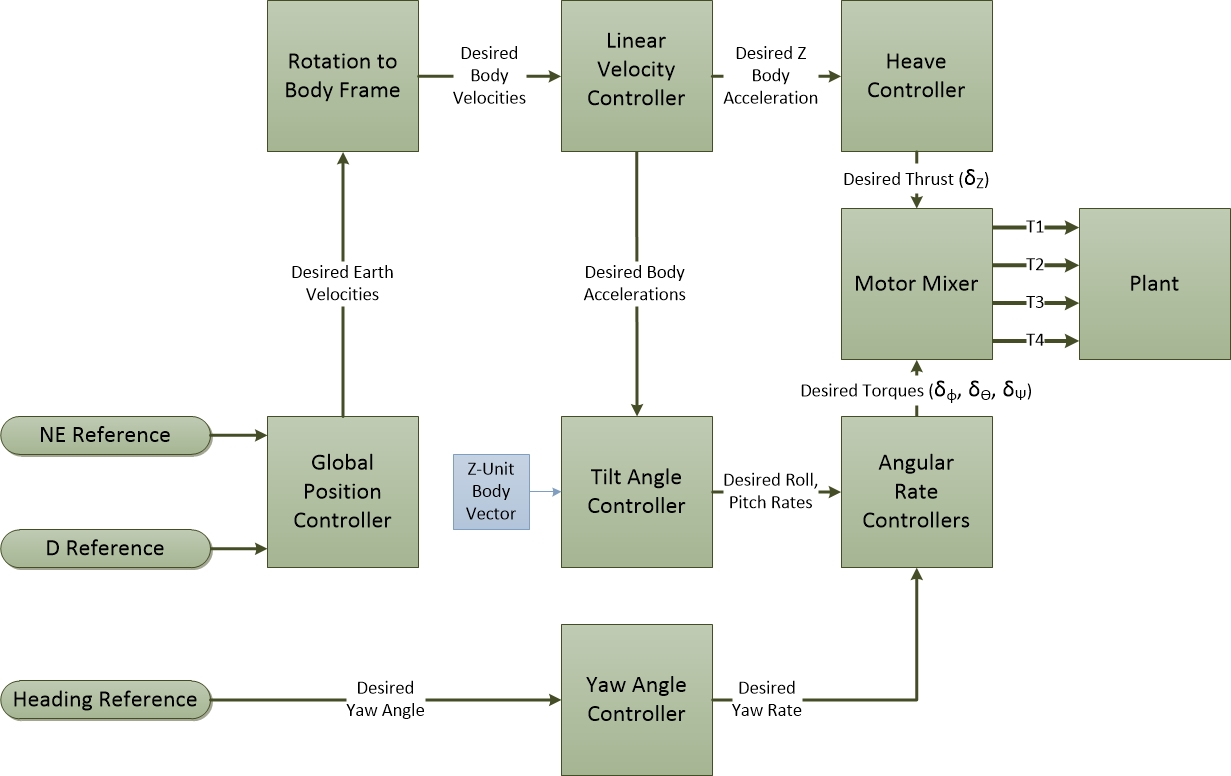
\includegraphics[height = 10cm]{../References/Diagrams/HighLevel.jpg}
	\caption{High Level Control Strategy}
	\label{IM_ControlStrategy}
\end{figure}

Each controller utilises the same rotor system to produce their outputs. This dependency on a single generation system allows for interference between the controllers. To ensure that no loop can saturate another, each system is given a percentage of headroom in which it can work, as shown in Table \ref{tab:HeadRoomPercentages}. The controller design must ensure that the thrust commanded during a step response is within those limits.

\begin{table}[H]
	\centering
	\begin{tabular}{l | c | c |}
		Controller 				& Percentage & Allowed Thrust Per Rotor\\
		\hline\hline
		Altitude 	   			& 64\% & 12.16N	\\
		North  		    		& 8\%  & 1.52N	\\
		East					& 12\% & 2.28N	\\
		Heading 		    	& 6\%  & 1.14N	\\
		Safety Factor 			& 10\% & 1.9N   \\
	\end{tabular}
	\caption{Thrust Headroom Controller Percentages}
	\label{tab:HeadRoomPercentages}
\end{table}

\section{Altitude Controller}
This section discusses the design and implementation of the altitude controller which is responsible for controlling the desired height of the craft. The craft is required to fly in confined spaces and must be able to track a setpoint with zero steady state error and negligible overshoot. In order for the altitude system to handle disturbances, an integrator term will be required. The system must be able to respond quickly to commands, however it must not exceed it's thrust utilisation percentage. To do this the system will require an upper limit which should not be reached. A lower limit is then introduced so the craft does not descend too quickly.

The overall altitude controller is structured as a set of cascaded control loops, with the most inner loop controlling the aircraft's acceleration and the most outer loop controlling the desired altitude in the earth frame. The system must be able to respond to disturbances quickly. Therefore, the inner heave loop utilises a PI controller to follow a desired vertical acceleration reference. The climb rate P controller is responsible for generating these acceleration references and is fed a desired linear vertical velocity reference by the altitude hold P controller. In order to reject measurement errors in the inner loops, the altitude hold controller makes use of a limited integrator that does effect the bandwidth of the system. Before the controller's can be designed, an analysis of the system's heave dynamics must first be performed.

\subsection{Heave Dynamics}
Using Newton mechanics at near hover conditions for the aircraft, the heave dynamics can be derived and are shown in \eqref{EQ_HeaveNewton}. Where $\dot{W}$ is the current acceleration of the craft in the Z-Axis and $m$ is the vehicles's mass. $Z$ is defined as the current instantaneous force being produced by the rotors.

\begin{equation}
\label{EQ_HeaveNewton}
\dot{W} = \dfrac{Z}{m}
\end{equation}

The state variable of the system is chosen as $Z$ with the output of this plant being $\dot{W}$. Using the transfer function for motor-rotor lag dynamics seen in \eqref{EQ_MotorDelay} and the dynamics seen in \eqref{EQ_HeaveNewton}, the state space equation for the system can be derived and is shown in \eqref{EQ_HeaveStateSpace1} and \eqref{EQ_HeaveStateSpace2}. 

\begin{eqnarray}
[\dot{Z}] &=& - [\dfrac{1}{\tau}] \ [Z] + [\dfrac{1}{\tau}] [\delta_Z]\label{EQ_HeaveStateSpace1}\\\label{EQ_HeaveStateSpace11}
[\dot{W}] &=& - [\dfrac{1}{m}] \ [Z]\label{EQ_HeaveStateSpace2}
\end{eqnarray}

Subsequently the transfer function can be calculated and the result is shown in \eqref{EQ_HeaveTF}. The negative gain of the transfer function must be noted and is caused by the direction of the defined axes, with the rotors producing a negative Z-Axis force.

\begin{equation}
G(s)_{heave} = \frac{\frac{-1}{m \times \tau}}{s + \frac{1}{\tau}}\label{EQ_HeaveTF}
\end{equation}

The rotor motor lag produces the pole at $\dfrac{-1}{\tau} = -8$ and indicates the maximum response capabilities and timing constant of the rotor system.

\subsection{Heave Controller}
The heave controller is responsible for commanding the $\delta_Z$ virtual actuator to achieve a desired Z-Axis acceleration in the body frame. The heave controller is the fastest controller in the altitude system and should utilise as much bandwidth as the rotor-motor system allows. The altitude controller wishes to reject disturbances quickly and thus a PI architecture was initially chosen as shown in Figure \ref{IM_HeaveController}. The system should be stable and exhibit a phase margin of at least $70$\textdegree.

The integrator is used to reject disturbances, while the most left limiter shown in Figure \ref{IM_HeaveController} was added to stop integrator wind up and is not considered during the linear controller design. The proportional gain is used to move the closed loop poles and achieve the desired bandwidth. The dynamic response of the system can be investigated using the root locus and bode plots shown in Figure \ref{IM_HeaveControlRoot} and \ref{IM_HeaveControlBode}. 

\begin{figure}[H]
	\centering
	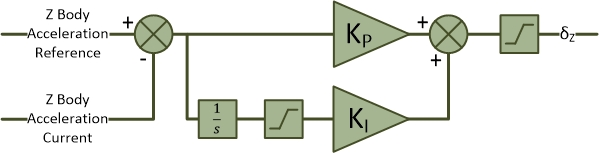
\includegraphics[height = 3.5cm]{../References/Diagrams/HeaveController.jpg}
	\caption{Heave Controller -  Control Diagram}
	\label{IM_HeaveController}
\end{figure}

Figure \ref{IM_HeaveControlRoot} shows the root locus of the system with the PI controller included. The controller introduces a new open loop pole at the origin. To maintain a first order response, the zero is placed close to the plant pole. This placement will attenuate the open loop, plant pole's response. Finally the gain is varied until the closed loop responses are closely aligned with the naturally occurring open loop pole. The final closed loop poles are a set of complex poles and are located at $-7.55 \pm 3.64 i$. The frequency response can be evaluated using the bode plot in Figure \ref{IM_HeaveControlBode}. 

\begin{figure}[H]
	\centering
	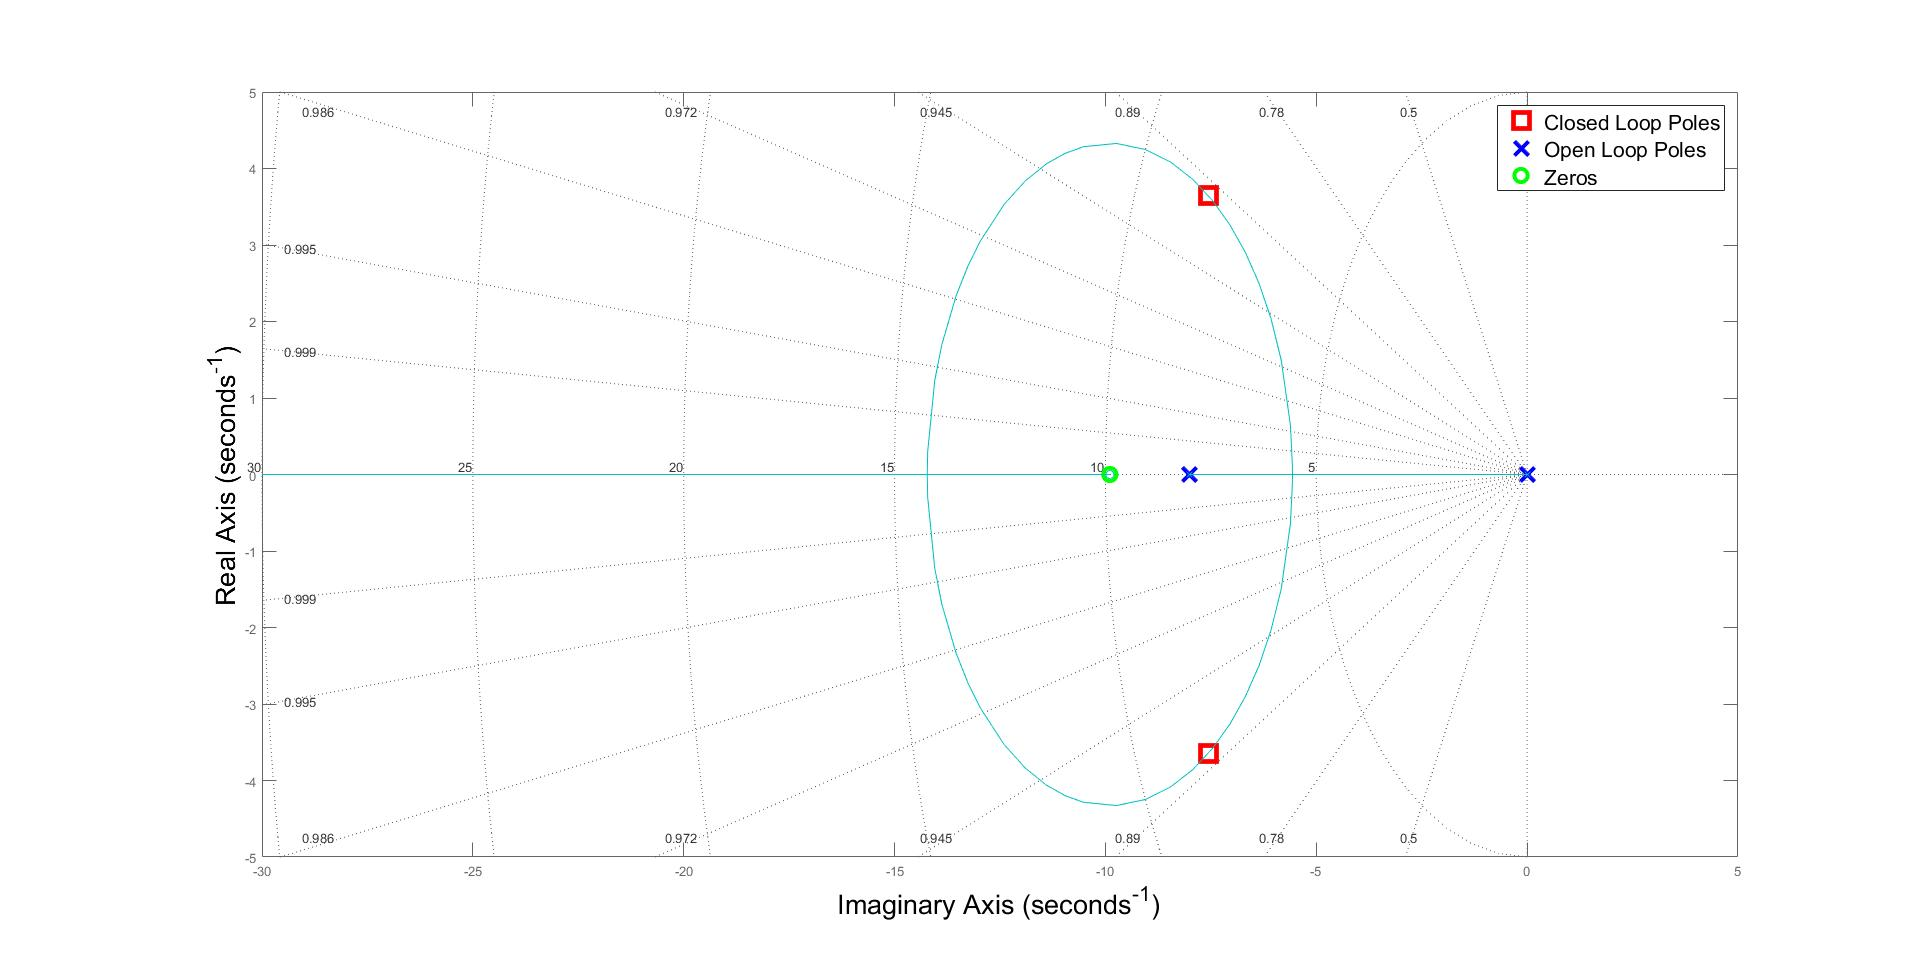
\includegraphics[height = 8cm]{../Design/Matlab/Controllers/heave_root.jpg}
	\caption{Heave Controller -  Root Locus}
	\label{IM_HeaveControlRoot}
\end{figure}

The final cross over frequency is shown on the bode plot for the heave controller in Figure \ref{IM_HeaveControlBode}. The gain plot shows the controller adjust the crossover frequency to $7.99$\,rad/s which is close to the limit of the system. The controller also increases the phase of the system and has a final phase margin of $84$\textdegree.

\begin{figure}[H]
	\centering
	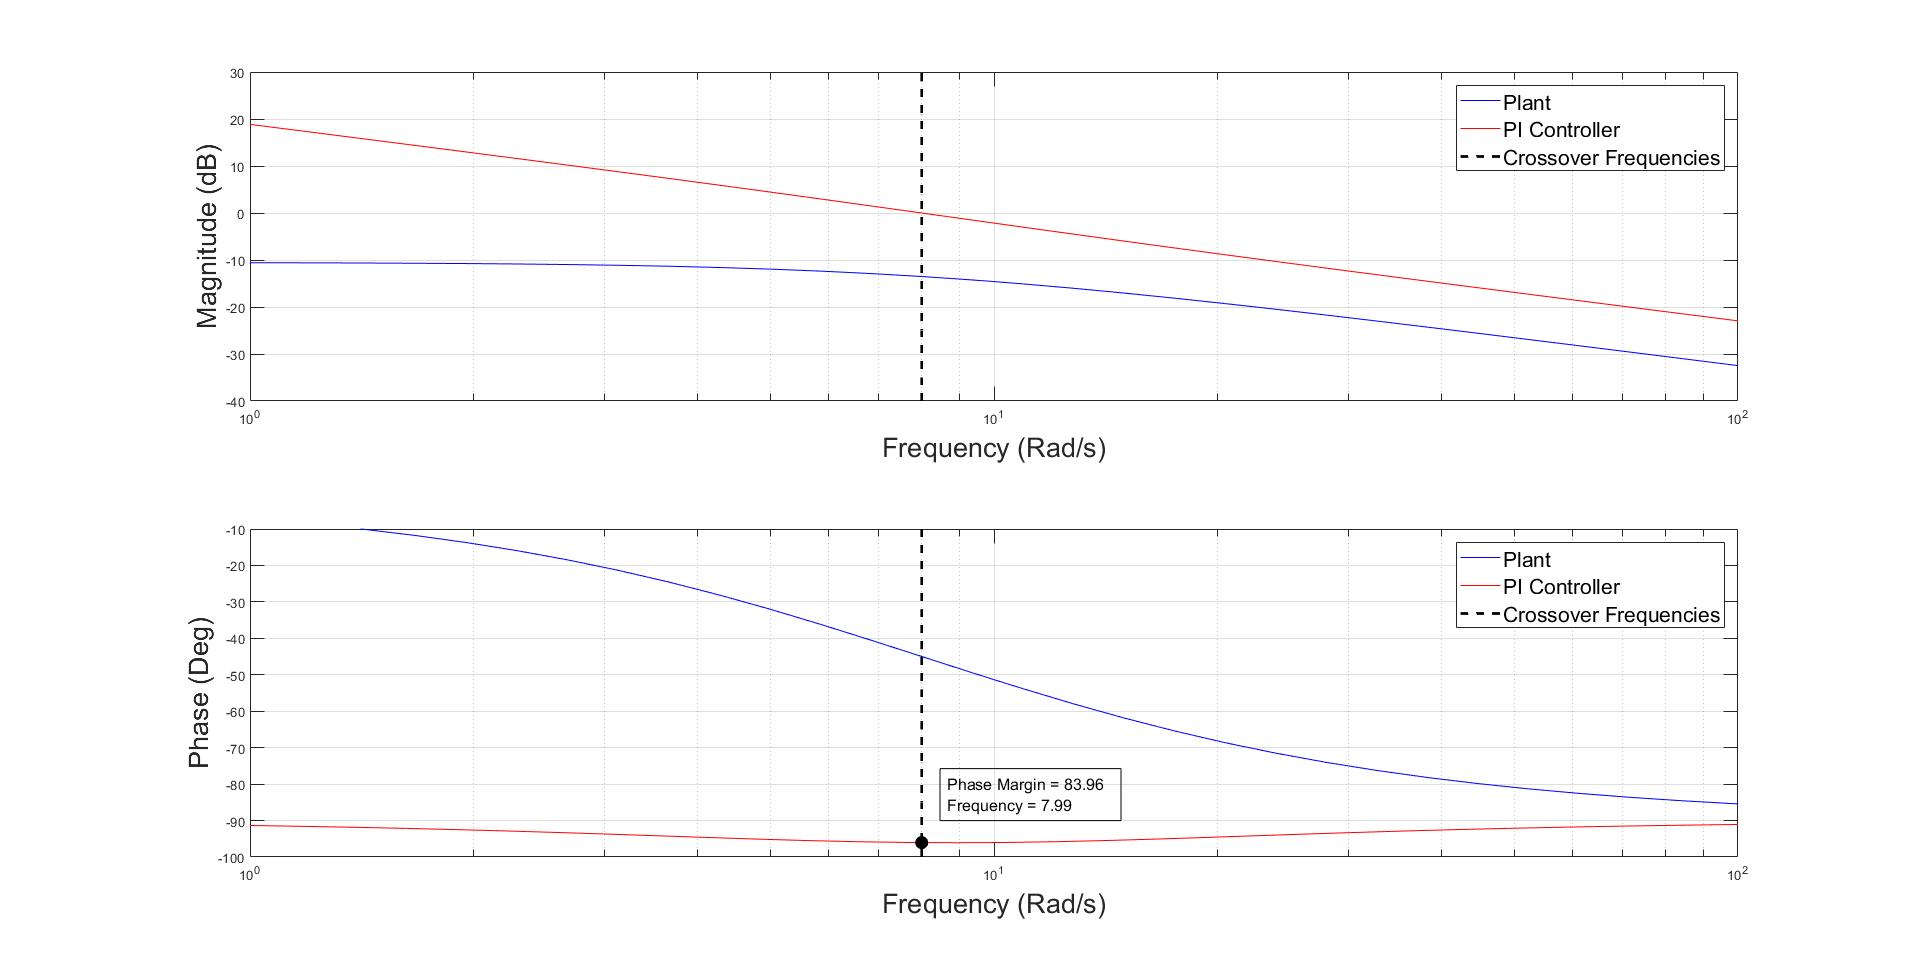
\includegraphics[height = 8cm]{../Design/Matlab/Controllers/heave_bode.jpg}
	\caption{Heave Controller -  Bode Plots}
	\label{IM_HeaveControlBode}
\end{figure}

An additional non linear element in the form of a limiter is brought into the system to limit the maximum and minimum thrust commands. The maximum limit is used to ensure the heave controller does not saturate the motors, thereby creating headroom for the angular rate controllers. The lower limit is used to ensure the vehicle always descends at a steady pace. The maximum thrust allowances are displayed in Table \ref{tab:HeadRoomPercentages}, the final limits chosen are shown in Table \ref{tab:HeaveLimits}.

\begin{table}[H]
	\centering
	\begin{tabular}{l | c | c |}
		Limit Name 				& Min & Max\\
		\hline\hline
		Integrator Wind Up 	   	& -1.5 	& 1.5 \\
		Thrust Command 		    & 10	& 48.64 \\
	\end{tabular}
	\caption{Heave Controller Limits}
	\label{tab:HeaveLimits}
\end{table}

\subsubsection{Heave Controller Discussion}
Now that the system presents stable dynamic results in the frequency and Laplace domains, using the non-linear simulation, the time domain responses can be discussed in brief. The resultant step response, including the PI controller, is shown in Figure \ref{IM_HeaveStepDist}. To demonstrate the disturbance rejection capabilities of the design, a force of $10N$ is applied to the drone at $2.5s$.

\begin{figure}[H]
	\centering
	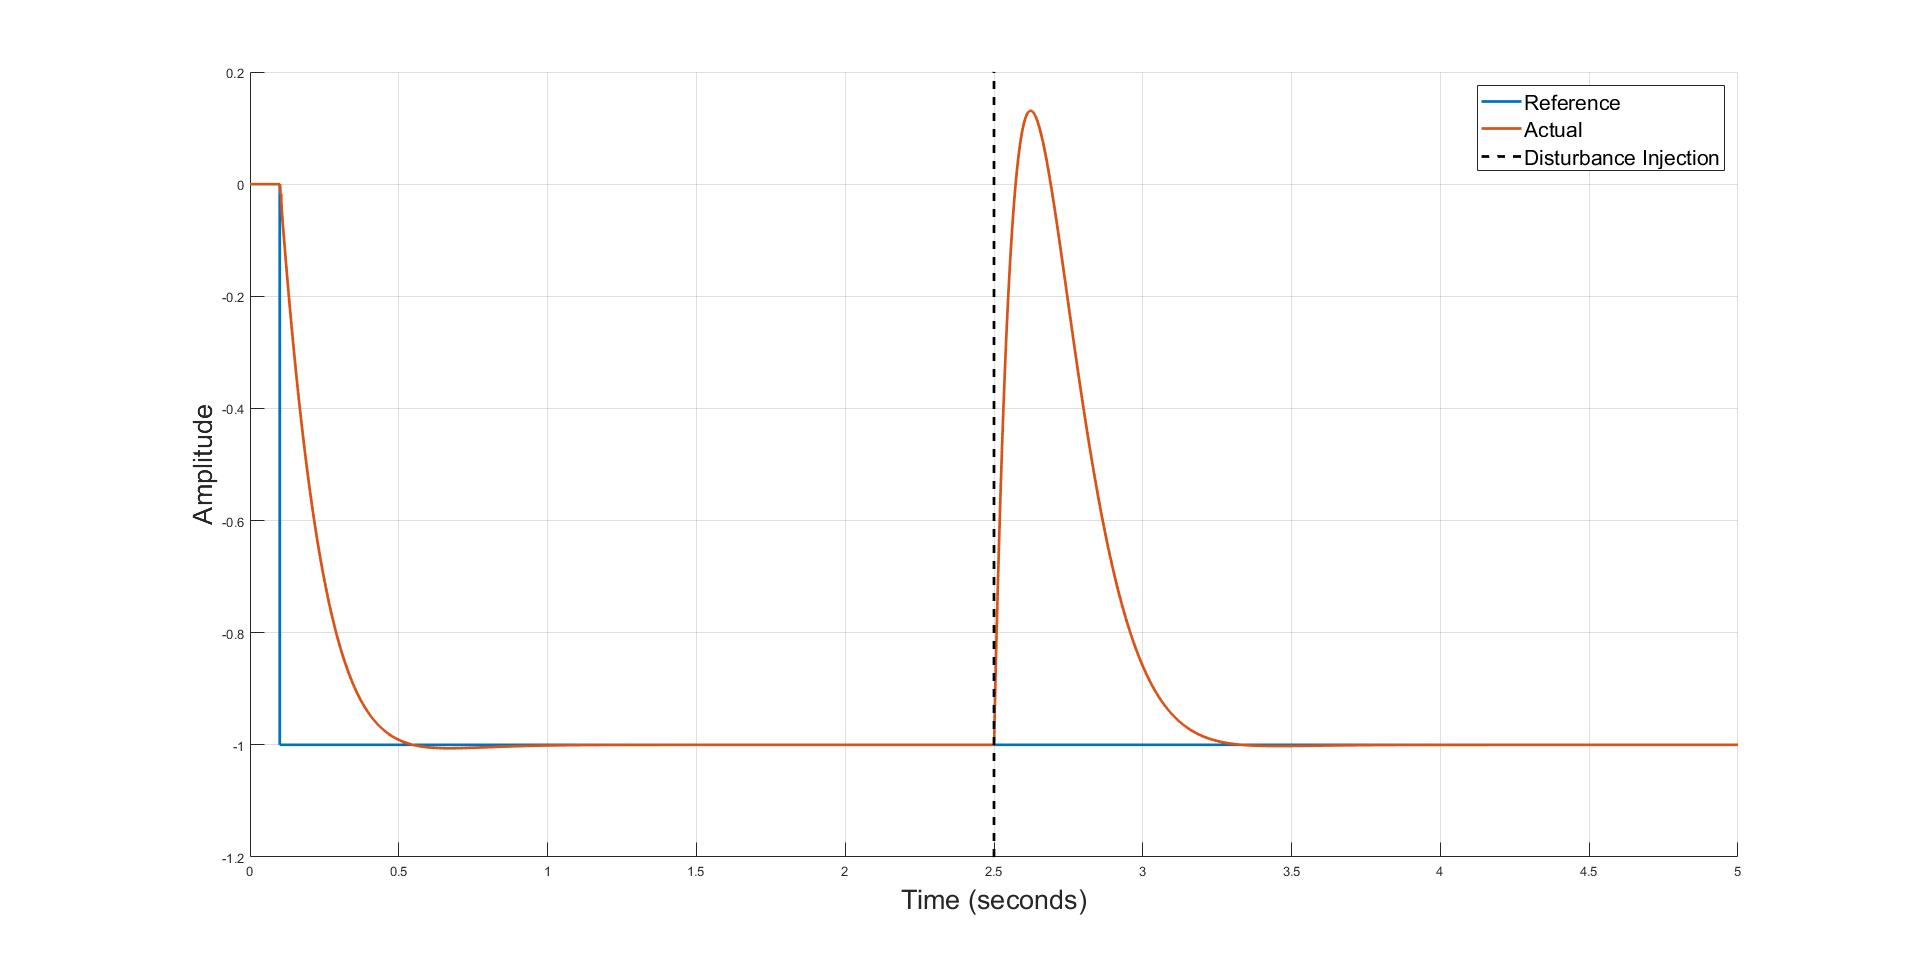
\includegraphics[height = 8cm]{../Design/Matlab/Controllers/heave_step.jpg}
	\caption{Heave Controller -  Step Response}
	\label{IM_HeaveStepDist}
\end{figure}

The heave controller, as the most inner loop, limits the response for the rest of the altitude control system. The proposed design brings the heave loop response close to the limits of the plant, thus producing a similar (but slower) timing constant to that of the motor-rotor system. The system reaches and settles within 5\% of the reference by $0.31s$, is critically damped and presents negligible overshoot. The system also shows to be capable of tracking an acceleration setpoint with zero steady state error. As shown in Figure \ref{IM_HeaveStepDist} the system can also respond quickly to a large, sudden and constant disturbance. The maximum rotor thrust commanded during this run is $3.35$\,N. \todo[inline]{How do I talk about gravity in this section? Can I just say gravity adds an offset of m*g and this plus the output must be less than the limit?}

\subsection{Climb Rate Controller}
The climb rate controller is responsible for controlling the vertical velocity of the aircraft, in the earth frame. This introduces the need for rotating either the reference or the command into the body frame. The decision can be made by considering the frame in which the sensing information is provided. Most aircraft make use of some form of global positioning system and using differentiation can calculate speed. However, due to the application environment, this aircraft will most likely use a velocity measurement sensor relative to the body frame. The architecture for the climb rate controller is outlined in Figure \ref{IM_ClimbRateControlLoop}. 

\begin{figure}[H]
	\centering
	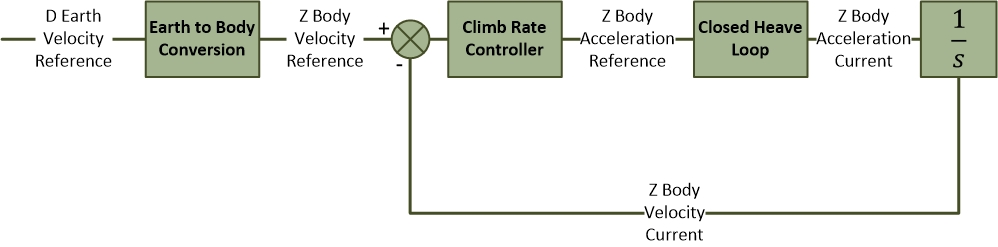
\includegraphics[height = 3.75cm]{../References/Diagrams/ClimbRateLoop.jpg}
	\caption{Climb Rate Controller Closed Loop}
	\label{IM_ClimbRateControlLoop}
\end{figure}

At near hover conditions the plant can be linearised and the rotation can be excluded. Figure \ref{IM_ClimbRateController} shows the simplified climb rate controller architecture. The computational time required for rotating the references can be considered by ensuring the controller design provides a reasonable phase margin. The speed of the climb rate controller is limited by the inner heave leave control loop. The controller must react quickly but there must still be a sufficient bandwidth ratio between the inner and outer loop. The controller must be able to track a setpoint with zero steady state error, but is not required to reject disturbances. The craft is required ot produce a steady approach to position targets, the climb rate controller should then exhibit a damped first order response.

\begin{figure}[H]
	\centering
	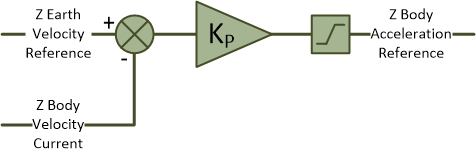
\includegraphics[height = 3.5cm]{../References/Diagrams/ClimbRateController.jpg}
	\caption{Climb Rate Controller}
	\label{IM_ClimbRateController}
\end{figure}		

The open loop poles of the climb rate system are located at the closed loop pole positions of the inner heave system, while the mathematical relationship between acceleration and velocity yields an additional open loop pole at the origin. The free integrator in the plant ensures the system will track a step response with zero steady state error while the proportional gain is used to speed up the system and achieve the desired bandwidth. The dynamic response of the system is evaluated using the root locus and bode plots shown in Figure \ref{IM_ClimbRateRoot} and \ref{IM_ClimbRateBode}.

\begin{figure}[H]
	\centering
	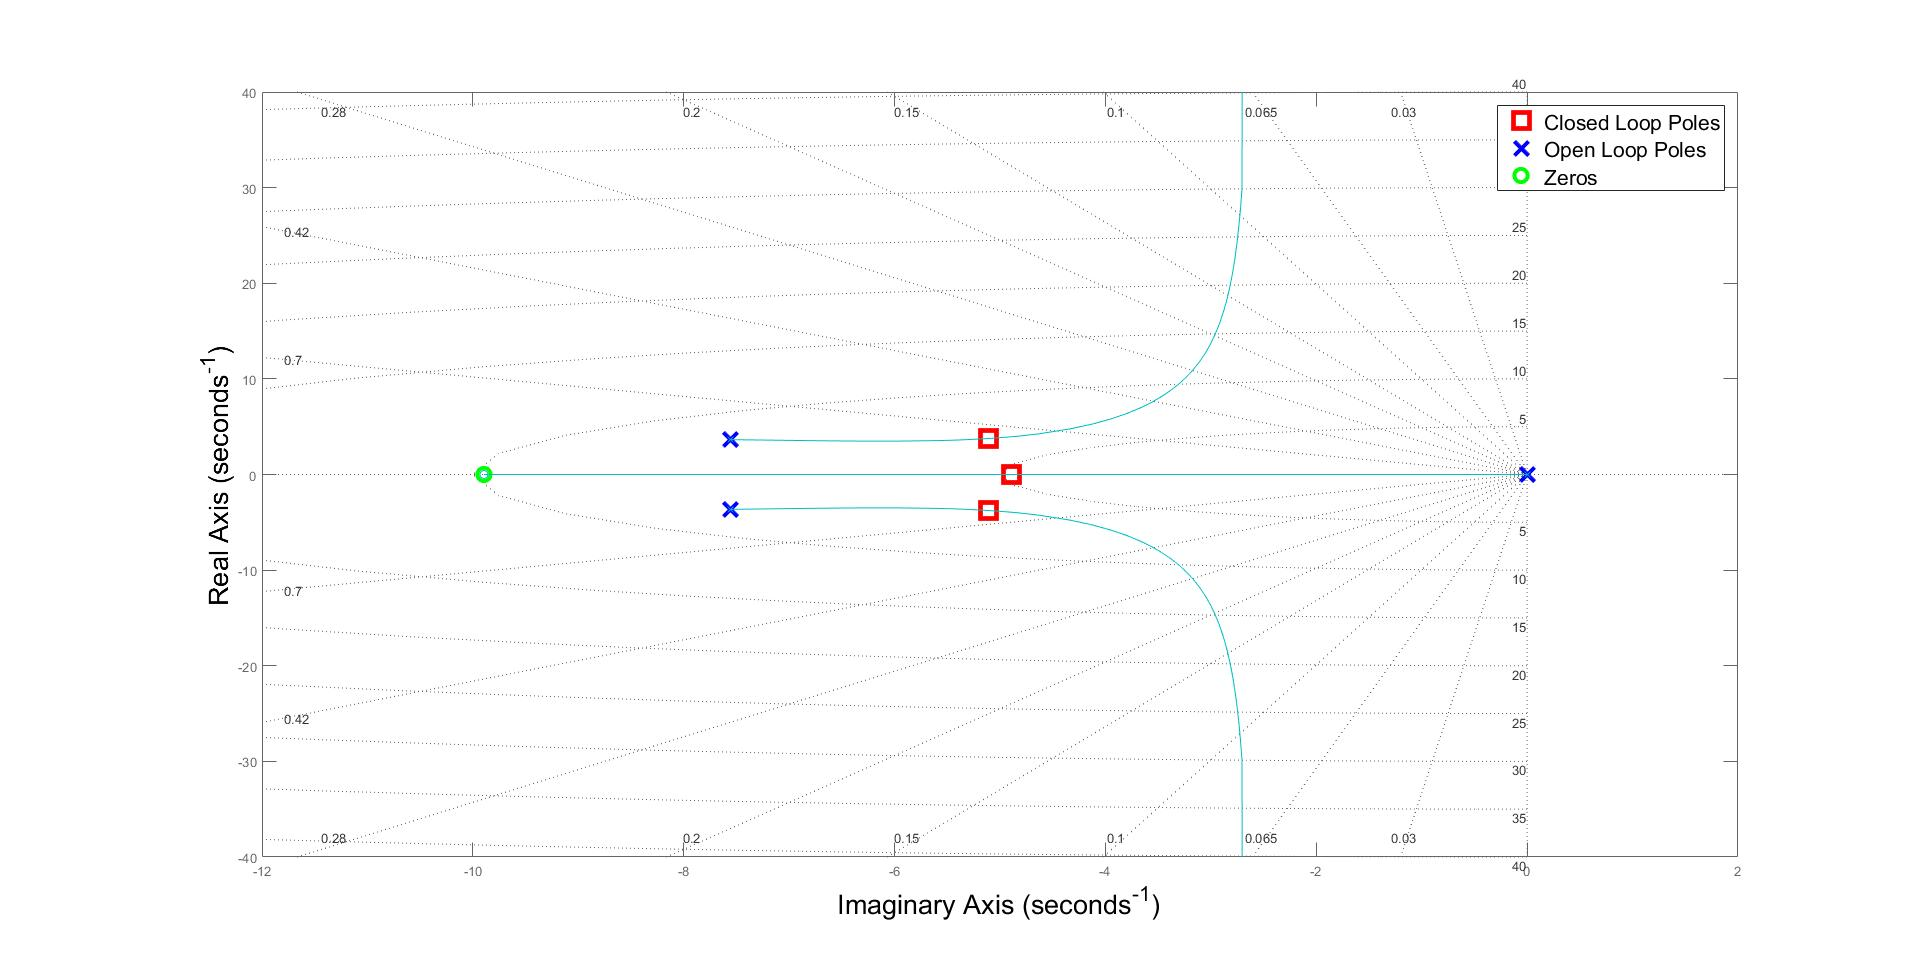
\includegraphics[height = 8cm]{../Design/Matlab/Controllers/climb_rate_root.jpg}
	\caption{Climb Rate Controller -  Root Locus}
	\label{IM_ClimbRateRoot}
\end{figure}

Figure \ref{IM_ClimbRateRoot} shows the location of the three final closed loop poles. There is a non dominant complex pair which is placed at $-5.11 \pm 3.76i$. The dominant pole is critically damped and located on the imaginary axis at $-4.89$.

\begin{figure}[H]
	\centering
	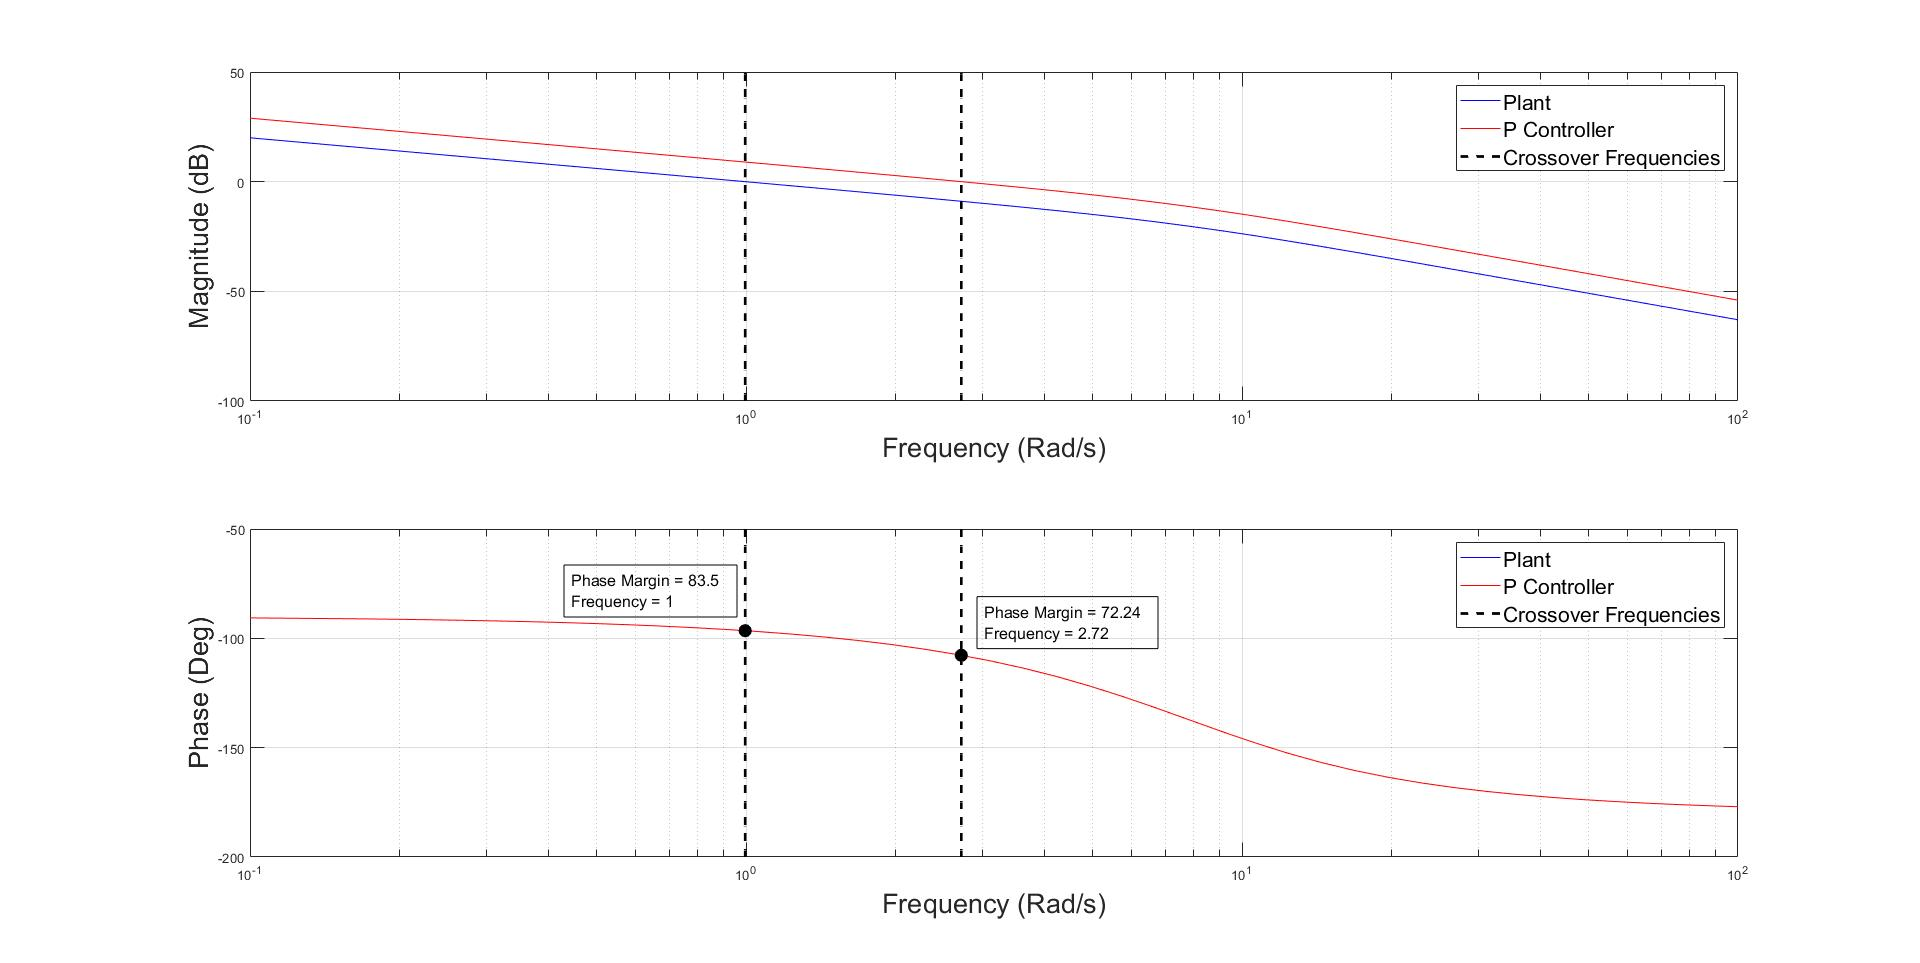
\includegraphics[height = 8cm]{../Design/Matlab/Controllers/climb_rate_bode.jpg}
	\caption{Climb Rate Controller - Open-Loop Bode Plots}
	\label{IM_ClimbRateBode}
\end{figure}

The bode plot shown in \ref{IM_ClimbRateBode} shows zero change in phase due to the controller architecture. The gain however is increased and moves the crossover frequency to $2.72$\,rad/s. The ratio of inner and outer loop crossover frequencies is then $2.91$, providing enough bandwidth between the inner and outer loops. The phase margin can then be calculated to be $72$\textdegree. 

As shown in Figure \ref{IM_ClimbRateController} there is a limiter applied to the acceleration commands. This limit is present due to the confined operational environment and ensures that the climb rate controller does not saturate the horizontal velocity controllers. The final limits are shown in Table \ref{tab:ClimbrateLimits}

\begin{table}[!]
	\centering
	\begin{tabular}{l | c | c |}
		Limit Name 						& Min & Max\\
		\hline\hline
		Acceleration Command 		    & -4 & 4 \\
	\end{tabular}
	\caption{Climb Rate Controller Limits}
	\label{tab:ClimbrateLimits}
\end{table}

\subsubsection{Climb Rate Controller Discussion}
The dynamic response shows sufficient phase margin to handle unmodelled timing delays. While the ratio between the inner controller ensures this controller will not be influenced by the inner loop. The step response of the closed loop system is shown in Figure \ref{IM_ClimbRateStep}. The system has a $5$\% settling time of $0.747s$ and shows negligible overshoot. At $5s$ a disturbance of $10N$ is placed on the rotors and the system demonstrates the ability to continue tracking the desired setpoint with zero steady state error. \todo[inline]{Not sure if I need the disturbance rejection here, maybe I could show that it can't handle a measurement error in the inner loop?}

\begin{figure}[H]
	\centering
	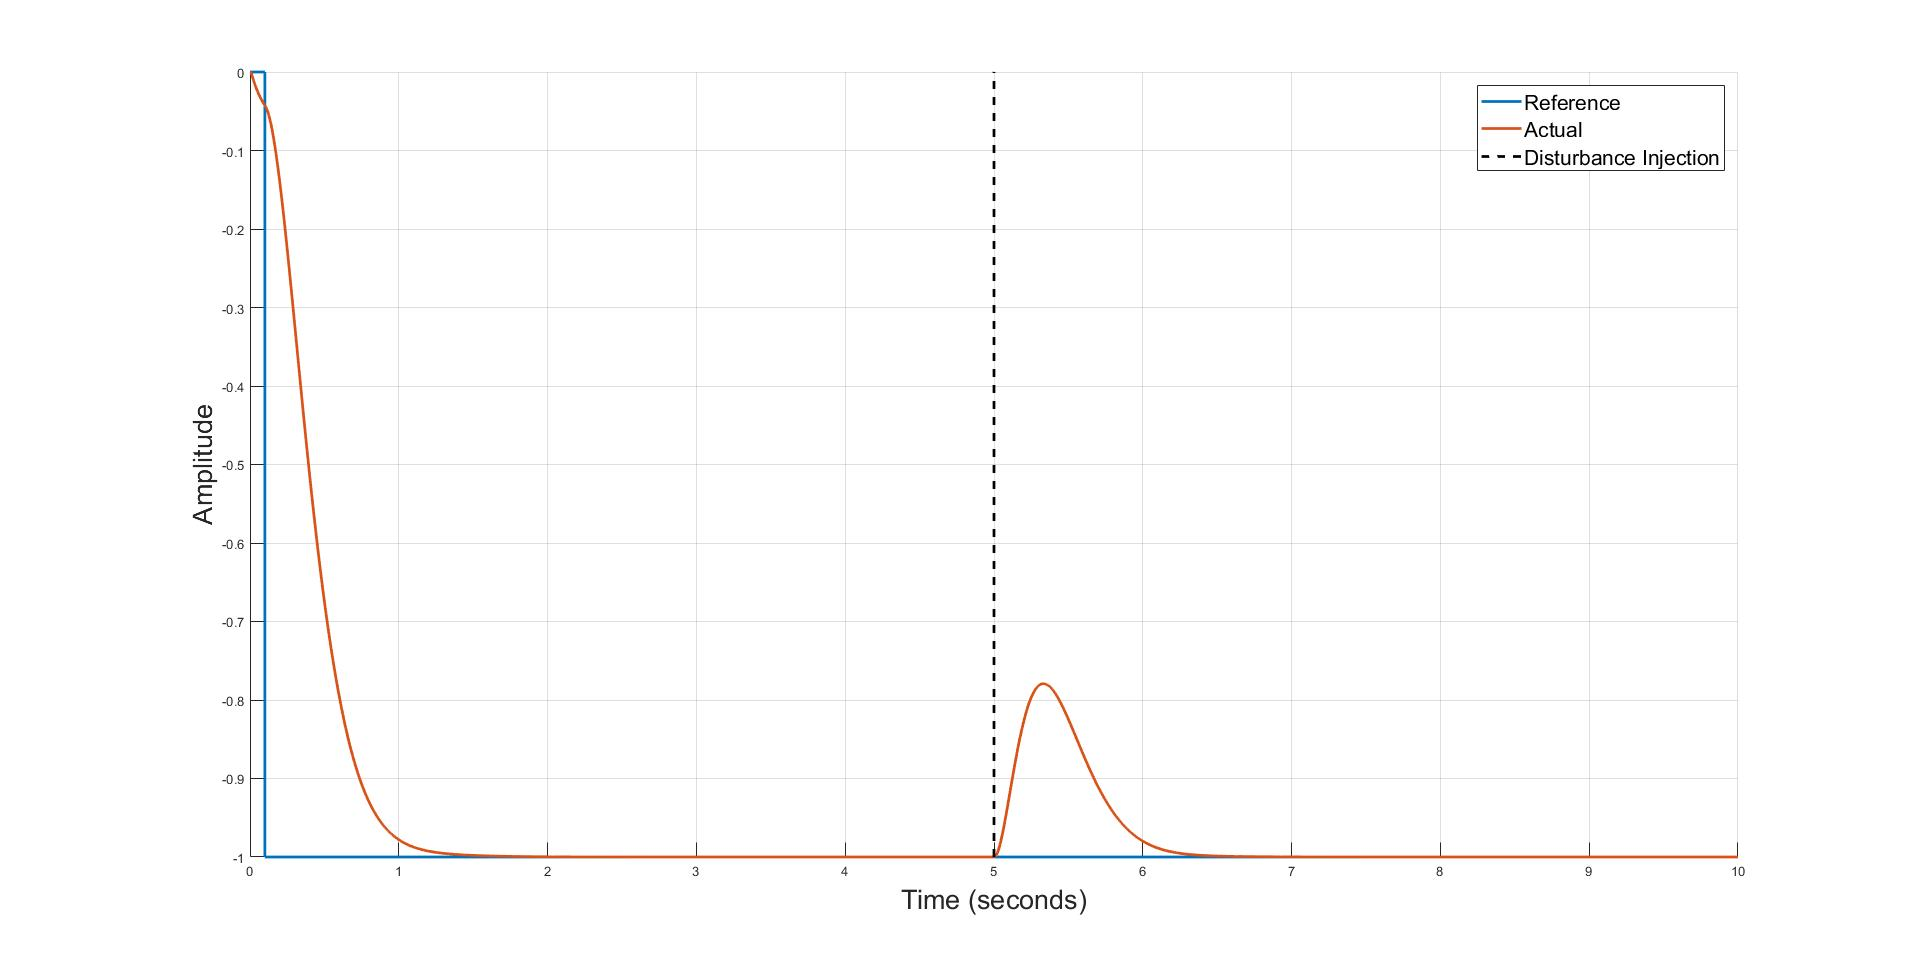
\includegraphics[height = 8cm]{../Design/Matlab/Controllers/climb_rate_step.jpg}
	\caption{Climb Rate Controller -  Step Response}
	\label{IM_ClimbRateStep}
\end{figure}

\subsection{Altitude Hold Controller}
The final stage of the vertical control system is the altitude hold controller. This controller receives a desired altitude in the earth frame and outputs a reference velocity, also in the earth frame. The closed control loop block diagram is shown in Figure \ref{IM_AltHoldControlLoop}. 

The altitude hold controller must be able to reject measurement errors in the inner loops, this can be achieved by adding an integrator into the controller. The system must also be able to track a set point with zero steady state error and must show a damped response with little overshoot. The system must be able to react quickly to commands, but is limited by the bandwidth of the climb rate system. The final bandwidth of this loop must be such that this controller is not influenced by the inner climb rate loop. As the most outer loop this system will have unmodelled errors, the controller must be robust and exhibit sufficient gain margin and a phase margin of at least $60$\textdegree.

\begin{figure}[H]
	\centering
	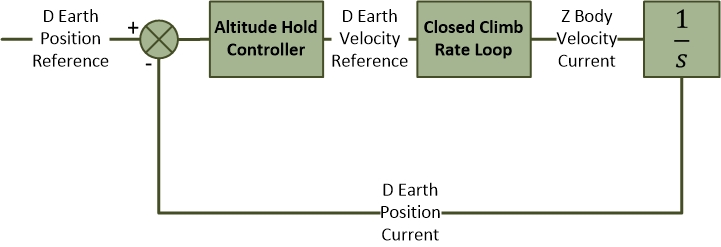
\includegraphics[height = 4cm]{../References/Diagrams/AltHoldLoop.jpg}
	\caption{Altitude Hold Controller Closed Loop}
	\label{IM_AltHoldControlLoop}
\end{figure}

The chosen controller architecture is shown in Figure \ref{IM_AltHoldController}. The proportional gain is used to vary the bandwidth to be within the limits of the system. An limited integrator is added to reject measurement errors in the inner loops, this component is represented by the faded integrator shown in Figure \ref{IM_AltHoldController} is not considered during linear analysis. The integrator shall be limited in such a way as to limit the interference of the proportional gain. This approach reduces the maximum disturbance rejection this controller can handle. To increase the bandwidth of the disturbance rejection capabilities, a PID controller architecture was also considered and the analysis was done for both control laws. \todo[inline]{Not sure if I should remove all the PID stuff here, I did consider it but the PID never stood a chance against the P and also do I need more disturbance rejection?}

The system's dynamic response is analysed using the root locus shown in Figure \ref{IM_AltHoldRoot} and the bode plot shown in Figure \ref{IM_AltHoldBode}.

\begin{figure}[H]
	\centering
	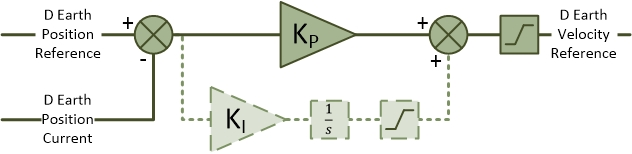
\includegraphics[height = 3.5cm]{../References/Diagrams/AltHoldController.jpg}
	\caption{Altitude Hold Controller}
	\label{IM_AltHoldController}
\end{figure}

Figures \ref{IM_AltHoldRoot} and \ref{IM_AltHoldBode} evaluate a P controller against a PID controller. The dominant closed loop poles of the P controlled system are placed at $-2.03 \pm 0.58i$ and are slightly under damped with a damping ratio of $0.96$. 

The PID controller adds an additional pole and two additional zeros into the system. The closed loop poles of the PID controlled system are located at $-6.64$, $-3.59 \pm 5.03i$ and $-0.64 \pm 0.47i$. The two new zeros are placed at $-0.57$ and $-2.06$.
\todo[inline]{Must decide if I must keep the PID stuff in and evaluate properly here}

\begin{figure}[H]
	\centering
	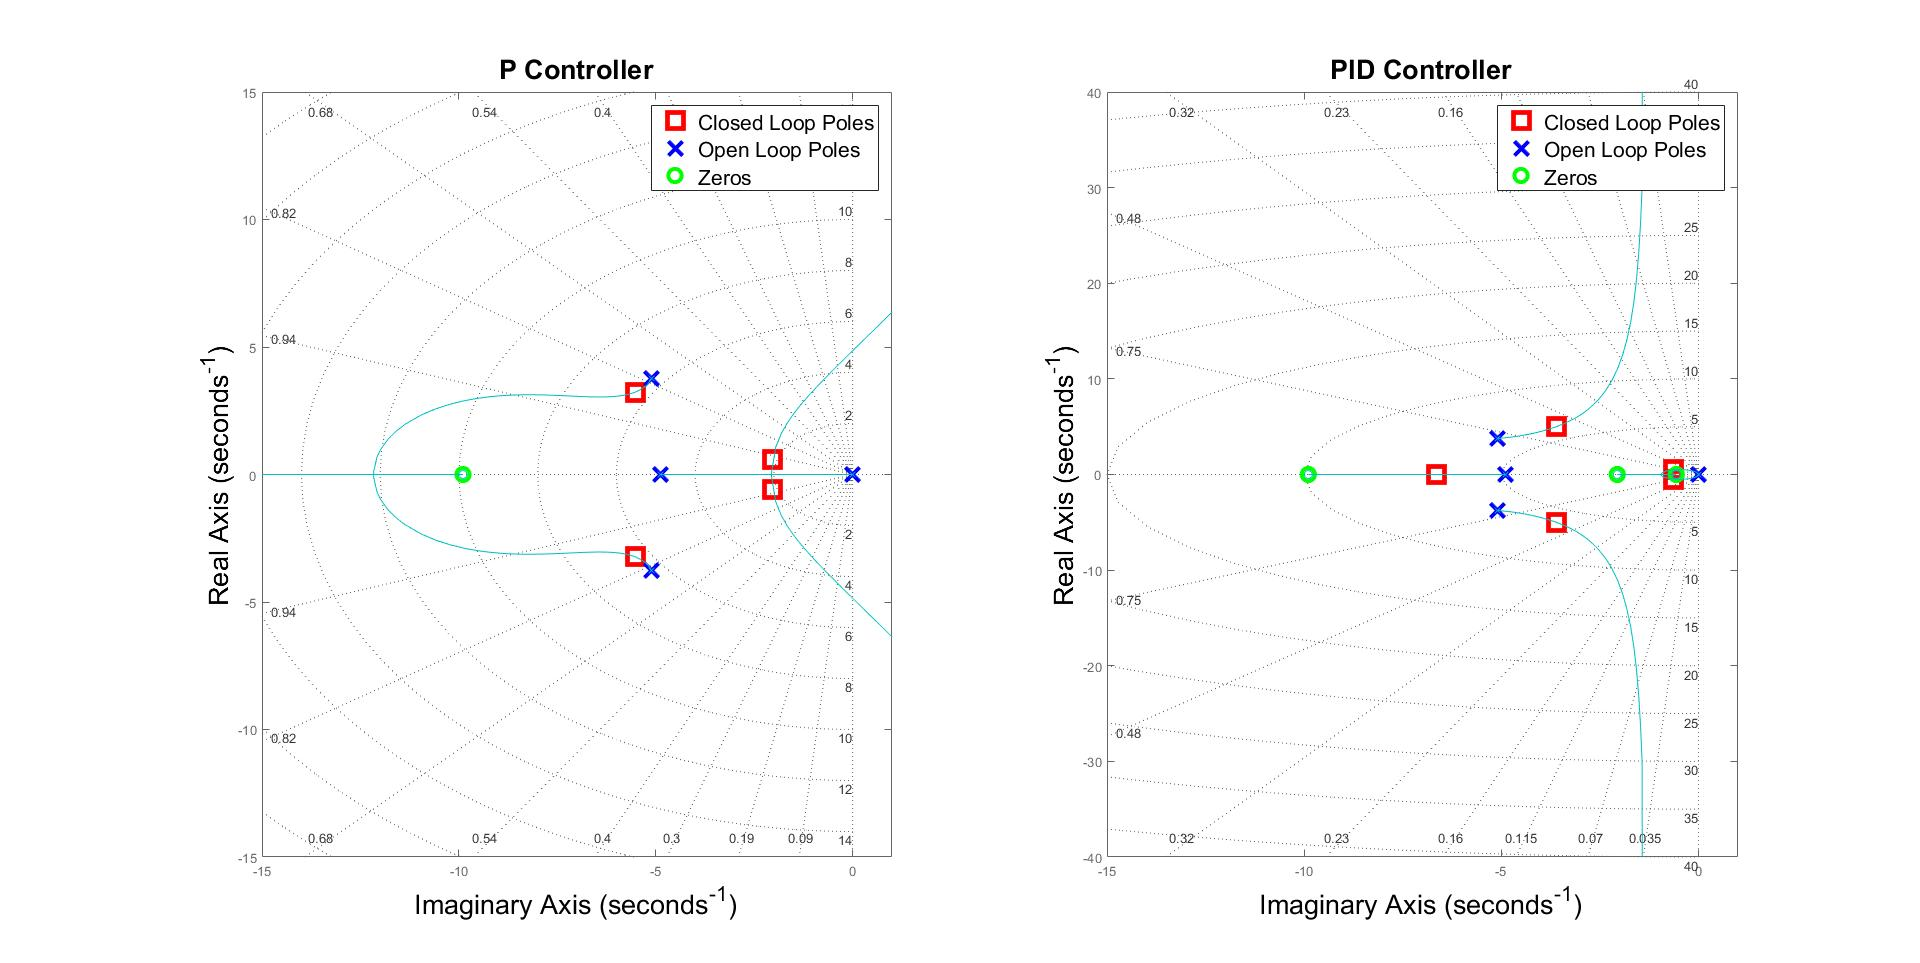
\includegraphics[height = 8cm]{../Design/Matlab/Controllers/altitude_root.jpg}
	\caption{Altitude Hold Controller -  Root Locus}
	\label{IM_AltHoldRoot}
\end{figure}

The bode plot shows the PID controller producing a final cross over frequency of $1.90Rad/s$, this response is too fast for the inner climb rate system and will need to be redesigned or discarded. \todo[inline]{Must decide if I must keep the PID stuff in and evaluate properly here}. The P controller exhibits a cross over frequency of $0.91Rad/s$, this produces a ratio of $3.03$ between the inner and outer loops and a phase margin of $71.5$\textdegree. The phase of the system using a P controller crosses the $180$\textdegree  $\ $mark at $4.81Rad/s$ and has a gain margin of $18.7dB$.

\begin{figure}[H]
	\centering
	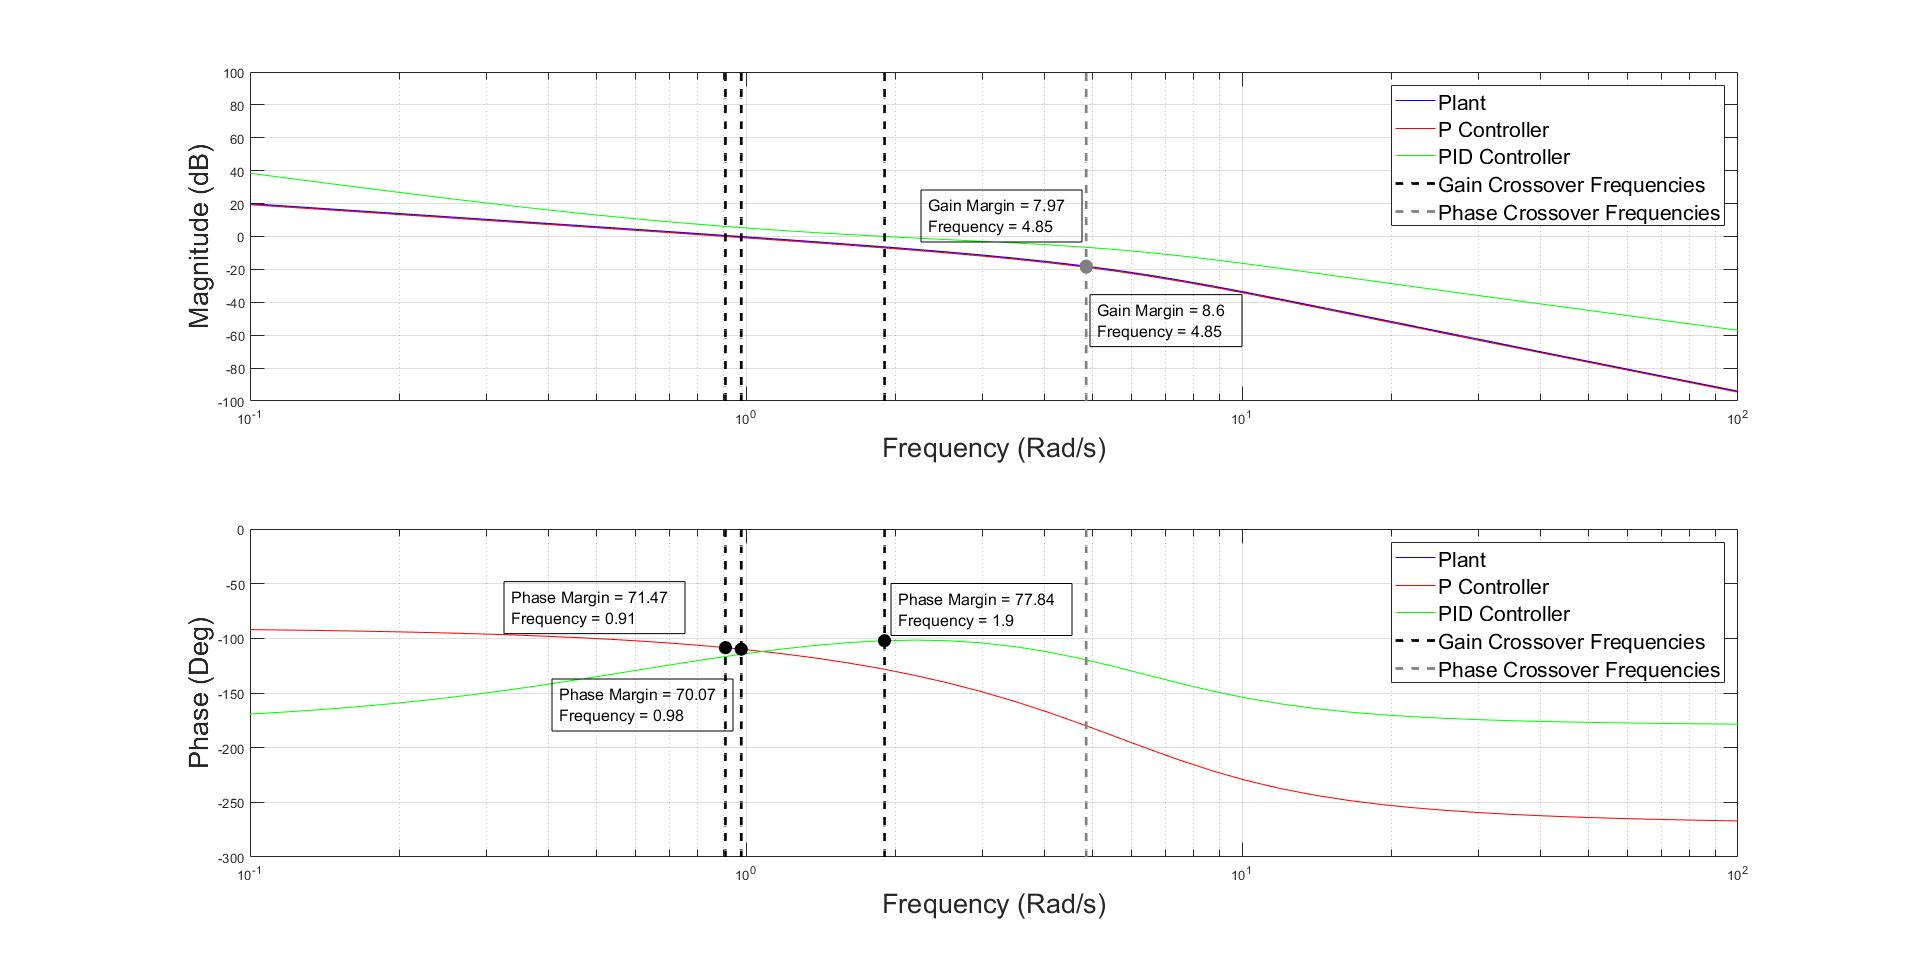
\includegraphics[height = 8cm]{../Design/Matlab/Controllers/altitude_bode.jpg}
	\caption{Altitude Hold Controller -  Bode Plots}
	\label{IM_AltHoldBode}
\end{figure}

To finalise the design, the two limiters are discussed. The first limiter is used to limit the effect of the integrator on the system as well as stop integrator wind up. The second limiter is used to limit the climb rate commands sent to the inner controllers. Both sets of limits are shown in Table \ref{tab:AltitudeControllerLimits}

\begin{table}[!]
	\centering
	\begin{tabular}{l | c | c |}
		Limit Name 						& Min & Max\\
		\hline\hline
		Integrator Wind Up 				& -0.09 & 0.09 \\
		Climb Rate Command 		    	& -5 & 5 \\
	\end{tabular}
	\caption{Altitude Hold Controller Limits}
	\label{tab:AltitudeControllerLimits}
\end{table}

\subsubsection{Altitude Hold Controller Discussion}
Although both the P and PID controllers exhibit stable dynamic responses, the PID controller exhibited too fast a response and will be influenced by the inner controllers. The system including only a P controller exhibits a step response as shown in Figure \ref{IM_AltHoldStep}, a disturbance of $10N$ is applied to the rotors at $10s$. The system has a $5\%$ settling time of $2.29s$ and tracks the set point with zero steady state error. The system handles the disturbance with a maximum overshoot of $0.01m$ and is close to being critically damped.

\begin{figure}[H]
	\centering
	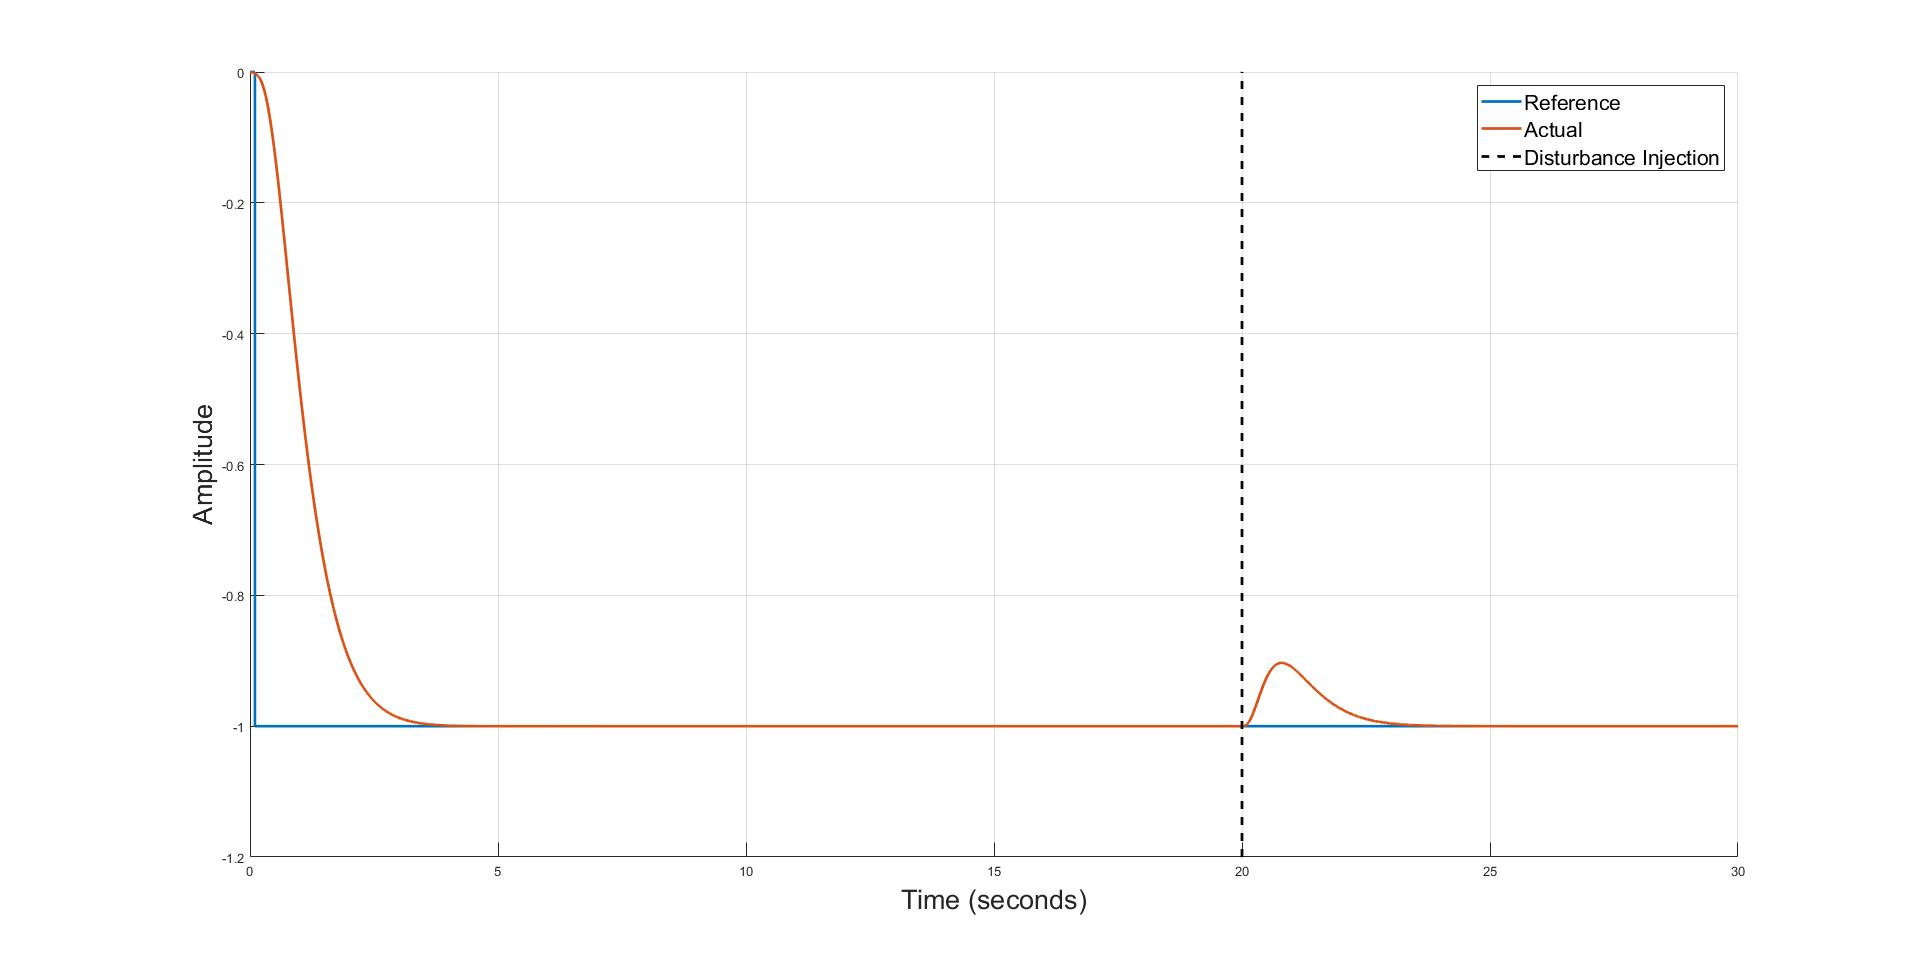
\includegraphics[height = 8cm]{../Design/Matlab/Controllers/altitude_step_p_no_dist.jpg}
	\caption{Altitude Hold P Controller -  Step response}
	\label{IM_AltHoldStep}
\end{figure}

However, if a measurement disturbance is present in the inner loops, this system will not track a setpoint with zero steady state error. To demonstrate this a constant offset of $0.05m/s$ is placed on the Z-Axis velocity measurement, Figure \ref{IM_AltHoldPDistStep} shows the current system cannot account for this disturbance. As shown in \ref{IM_AltHoldController}, a limited gain integrator is introduced into the system to help the system track steady state error. 

\begin{figure}[H]
	\centering
	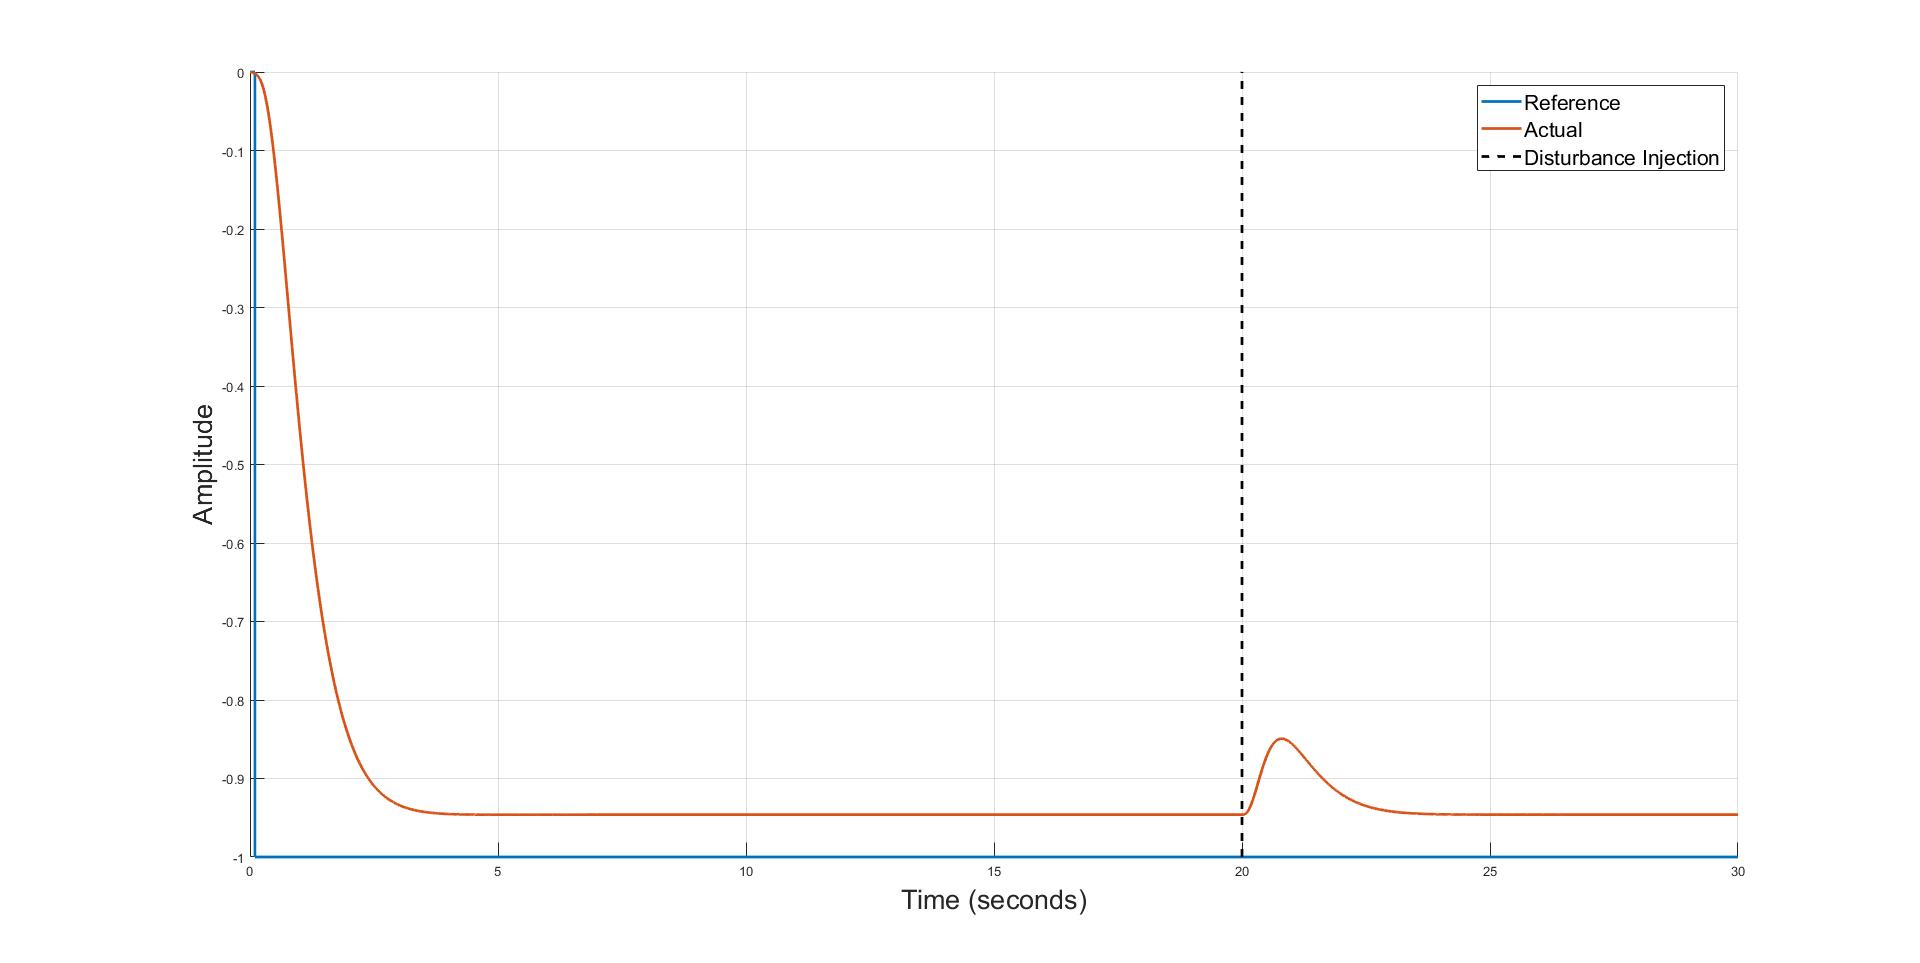
\includegraphics[height = 8cm]{../Design/Matlab/Controllers/altitude_step_p_dist.jpg}
	\caption{Altitude Hold P Controller -  Step response with inner loop measurement offset}
	\label{IM_AltHoldPDistStep}
\end{figure}

The new controller must be limited in such a way as to exhibit a similar transient response as the existing P controller. Figure \ref{IM_AltHoldPIDistStep} shows the step response of the new system both with and without the $0.05m/s$ offset in the velocity measurement. As shown, the P controller including a limited I component introduces more overshoot into the system. The limits are designed to ensure the new controller introduces less than 10\% overshoot into the system. 

\begin{figure}[H]
	\centering
	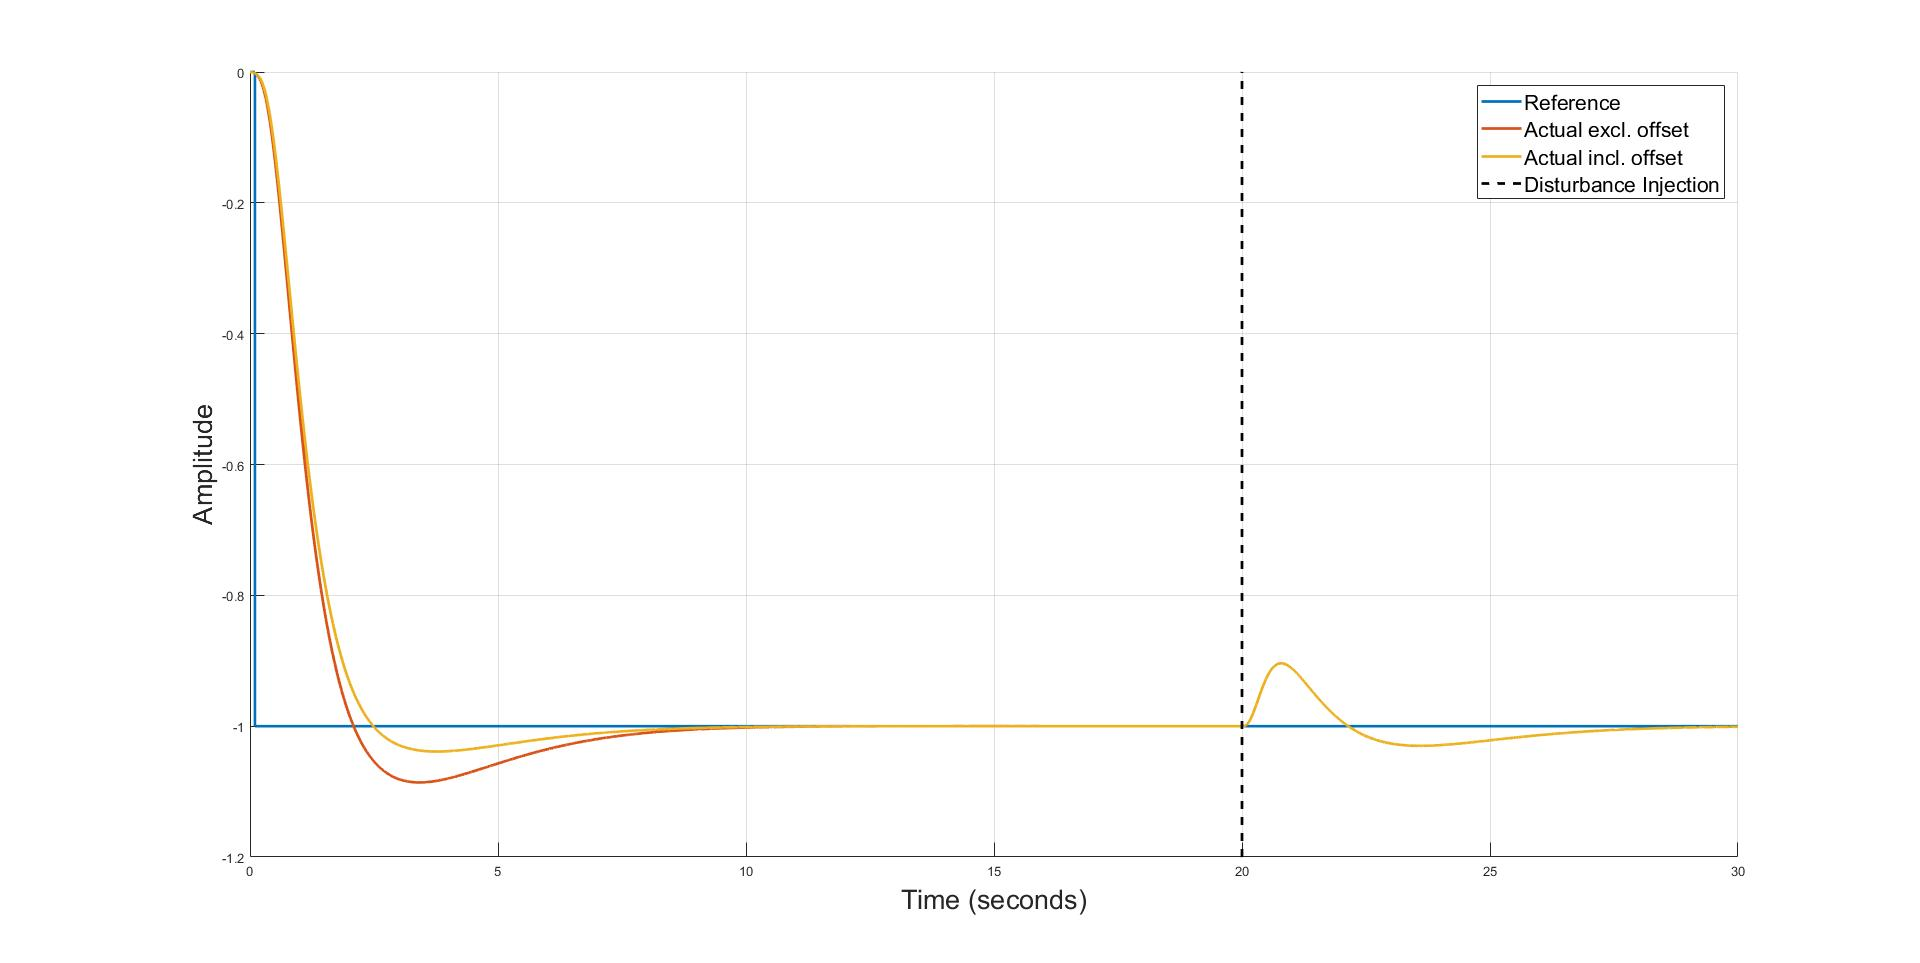
\includegraphics[height = 8cm]{../Design/Matlab/Controllers/altitude_step_pi.jpg}
	\caption{Altitude Hold P with Limited I Controller -  Step Responses}
	\label{IM_AltHoldPIDistStep}
\end{figure}

\todo[inline]{Do I need to show impulse responses for altitude and climb rate? I mention the maximum thrust at the heave controller level, is that good enough?}

\section{Horizontal Control}
\todo[inline]{Incomplete, skip this section please}
This section describes the horizontal controller. This system is responsible for controlling the craft's North and East position in the earth frame, to do this the controller commands the pitch and roll rates. The horizontal controller is designed as two sets of four cascaded control loops, one set for roll and one set for pitch. The most inner loop controls either the roll or pitch rate of the craft by commanding the virtual actuators $\delta_\phi$ and $\delta_\theta$ respectively. The desired angular rates are commanded by the tilt angle controller. The tilt angle controller is responsible for converting a desired translational acceleration into desired roll and pitch angles. The linear velocity controller receives it's setpoint from the most outer global position controller. 

\subsection{Roll and Pitch Rate Dynamics}
The roll and pitch acceleration dynamics can be derived using Newton mechanics at near hover conditions and the craft's inertia around the X-axis ($I_{xx}$) and the Y-axis ($I_{yy}$) respectively, the result is shown in \eqref{EQ_RollNewton} and \eqref{EQ_PitchNewton}.

\begin{equation}
\label{EQ_RollNewton}
\dot{p} = \dfrac{L}{I_{xx}}
\end{equation}

\begin{equation}
\label{EQ_PitchNewton}
\dot{q} = \dfrac{M}{I_{yy}}
\end{equation}

The rotors introduce an additional timing delay into the dynamics. The state space equation for both systems can be derived using the current angular rates ($p$ \& $q$) and the current angular moments ($L$ \& $M$) as the system states. The state space representation for roll is shown in \eqref{EQ_RollStateSpace1} and \eqref{EQ_RollStateSpace2}. The transfer function for roll acceleration can be calculated from the state space representation, integrating the result produces the transfer function for roll rate as shown in \eqref{EQ_RollTF}. The same approach is followed for deriving the pitch rate dynamics.

\begin{eqnarray}
\begin{bmatrix} \dot{L} \\ \dot{p}	\end{bmatrix}&=&\begin{bmatrix}\frac{1}{\tau}\ \ \ \ \ 0\\\frac{1}{I_{xx}} \ \ \ 0 \end{bmatrix} \begin{bmatrix} L \\ p \end{bmatrix} + \begin{bmatrix}\frac{1}{\tau}\\ 0 \end{bmatrix} \delta_\phi\label{EQ_RollStateSpace1}\\\label{EQ_RollStateSpace11} 
y &=& \begin{bmatrix} 0 \ \ \ \ 1 \end{bmatrix} \begin{bmatrix} L \\ p \end{bmatrix} \label{EQ_RollStateSpace2}\\
G(s) &=& \frac{\frac{1}{\tau I_{xx}}}{s (s + \frac{1}{\tau})}\label{EQ_RollTF}
\end{eqnarray}

The roll and pitch plants both have a naturally occurring integrator, an open loop pole at $-\dfrac{1}{\tau}$ and no naturally occurring zeros. As shown, the plant gain is inversely proportional to the specific axis inertia. The design of the craft creates a much larger pitching plant gain than rolling plant gain. The controller must compensate for this, resulting in similar closed loop system responses for both roll and pitch rate.

\subsection{Roll Rate Controller}
The roll rate controller is one the most inner loops of the horizontal controller and commands the $\delta_\phi$ virtual actuator. As the most inner controller the outer loops are limited by this system's response and bandwidth. To speed up the system a lead compensator is added in series with a proportional controller. An integrator is included to reject disturbances and eliminate steady state error, the final controller is shown in Figure \ref{IM_RollRateController}.

\begin{figure}[H]
	\centering
	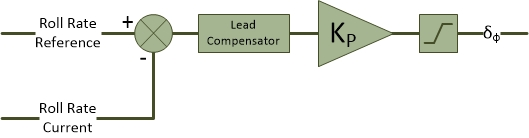
\includegraphics[height = 3.3cm]{../References/Diagrams/RollRateController.jpg}
	\caption{Roll Rate Controller}
	\label{IM_RollRateController}
\end{figure}	

The dynamic response of both the Lead-P and Lead-PI controlled systems are evaluated using the root locus in Figure \ref{IM_RollRateControlRoot}. The root locus diagram of the Lead-P controller shows how the placement of the lead compensator zero cancels the naturally occurring open loop pole at $-\dfrac{1}{\tau}$. To align the closed loop poles closely with the physical limit of the system, the pole of the compensator is placed at $-\dfrac{2}{\tau}$. 

The additional poles and zeros in the Lead-PI system require a slightly different approach. There are now two dominant poles that sit close to the origin, to maintain a first order response, the two dominant poles are kept close to the imaginary axis assisted by the integral zero. The placement of the integral zero also dictates how aggressively the system will respond to disturbances. The final placement of the integral zero is $-1$\,rad/s and the compensator zero is moved to $-5.7$\,rad/s.

\begin{figure}[H]
	\centering
	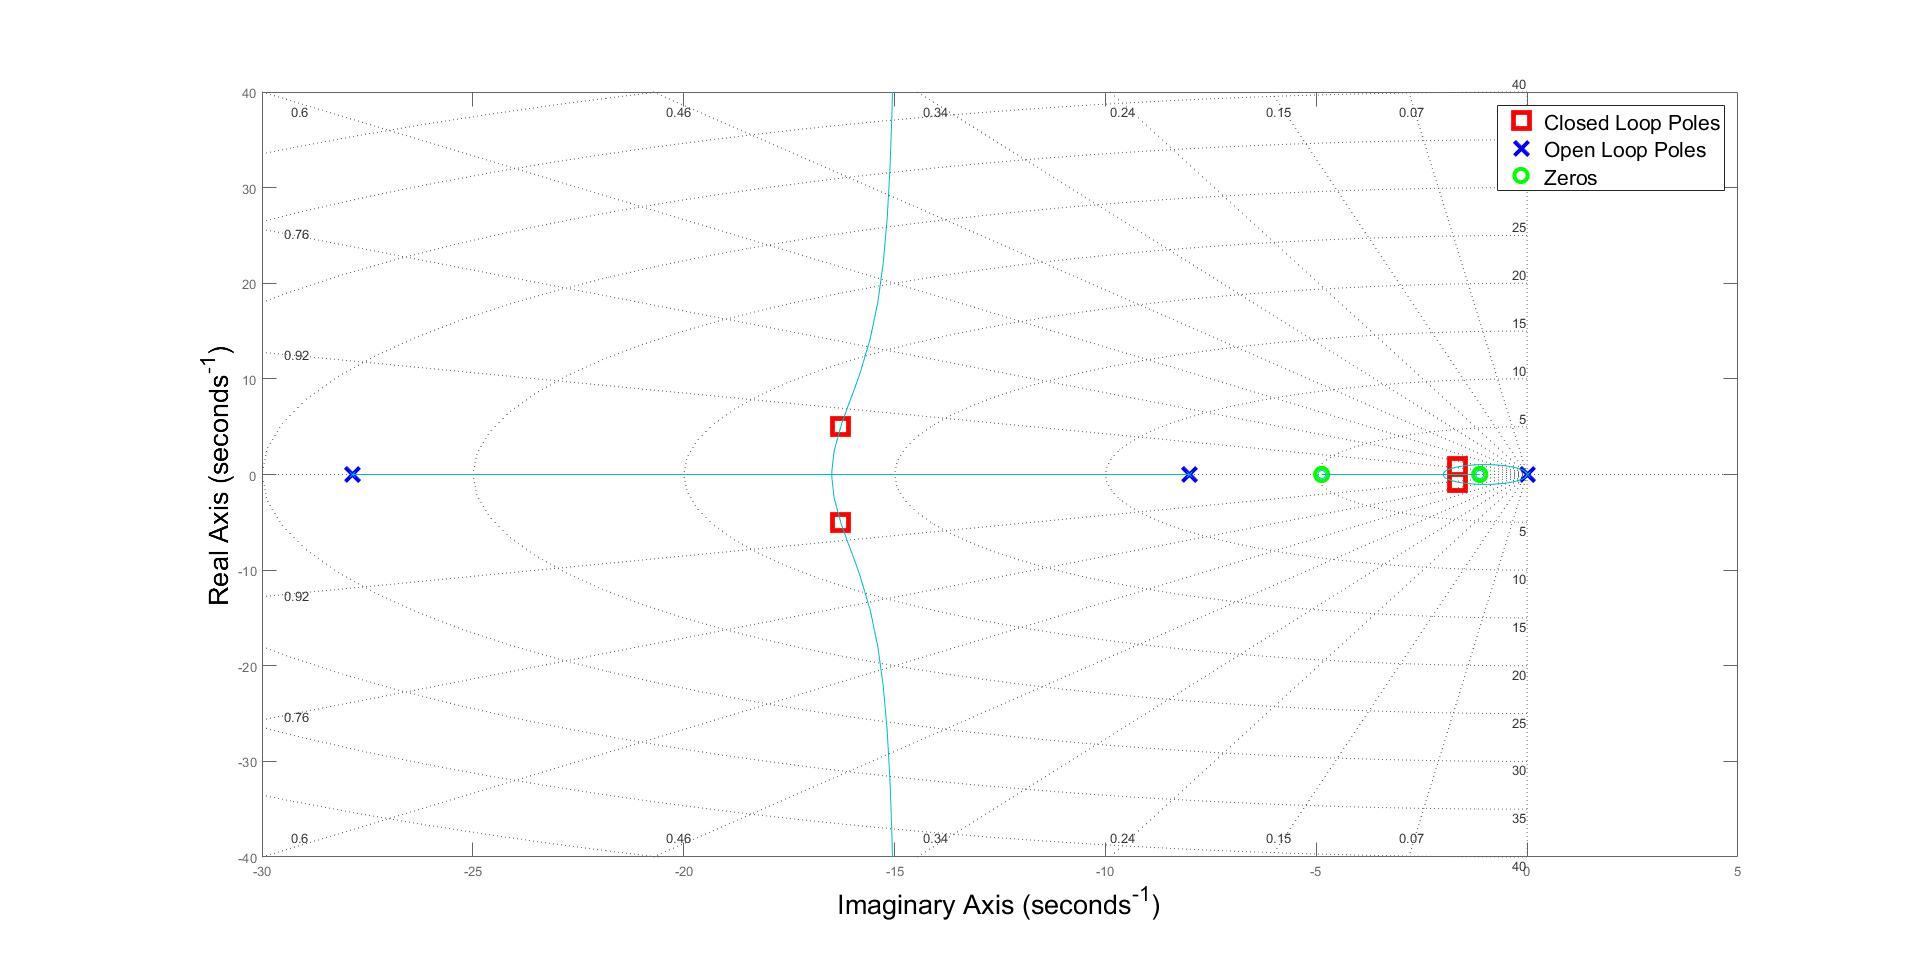
\includegraphics[height = 8cm]{../Design/Matlab/Controllers/roll_rate_root.jpg}
	\caption{Roll Rate Controller -  Root Locus (Left:Lead-P, Right:Lead-PI)}
	\label{IM_RollRateControlRoot}
\end{figure}

The frequency response of the system is investigated using the bode plot shown in Figure \ref{IM_RollRateControlBode}. Unity feedback is compared against three seperate controllers. A standard Proportional (P) controller, a P controller including a lead-compensator and finally, the chosen control law, a Proportional Integral (PI) controller preceded by a lead compensator. As shown unity feedback produces a stable result, however there is an insufficient phase margin of $58$\textdegree in the system. Proportional control can increase the phase margin by reducing the bandwidth, however this slows the system to an unacceptable level, with a cross-over frequency of $2.32$\,rad/s. To compensate for this a lead compensator is added to increase the phase of the system while maintaining the bandwidth. The system now has sufficient bandwidth and phase of $73$\textdegree at $4.81$\,rad/s however, it will be prone to disturbances.  The Lead-PI adds an integrator and has a final phase margin of $70$\textdegree with a crossover frequency of $4.67$\,rad/s.

\begin{figure}[H]
	\centering
	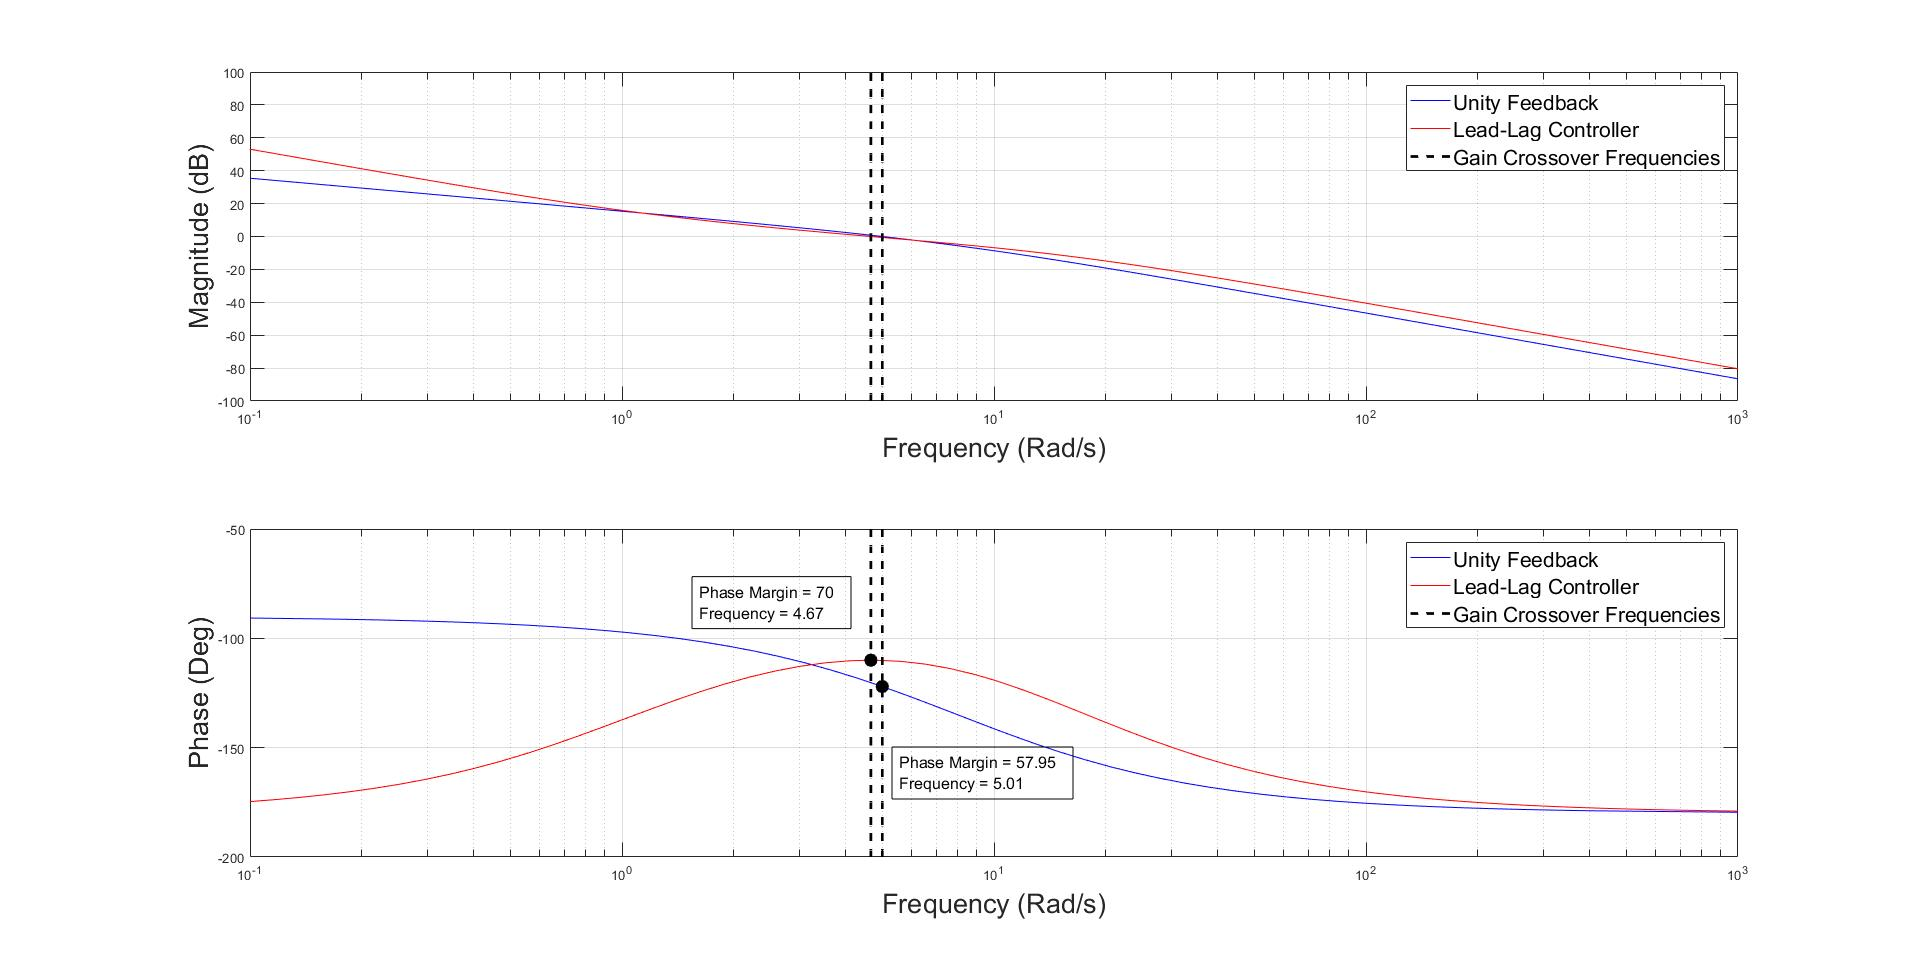
\includegraphics[height = 8cm]{../Design/Matlab/Controllers/roll_rate_bode.jpg}
	\caption{Roll Rate Controller -  Bode Plots}
	\label{IM_RollRateControlBode}
\end{figure}

\subsubsection{Roll Rate Controller Discussion}
Two designs for the roll rate controller were investigated, both producing stable responses. The Lead-P controller produces the fastest and most stable response however it will be prone to disturbances. These disturbances can be accounted for by an outer loop, however it is desired for the system to respond to disturbances quickly. This calls for the addition of an integral term in the inner rate system. 
The integral term in the Lead-PI controller has a non-linear saturation to limit the overshoot introduced by the integral term. The step response for each described system is shown in Figure \ref{IM_RollRateStep}, including the unlimited Lead-PI system.

\begin{figure}[H]
	\centering
	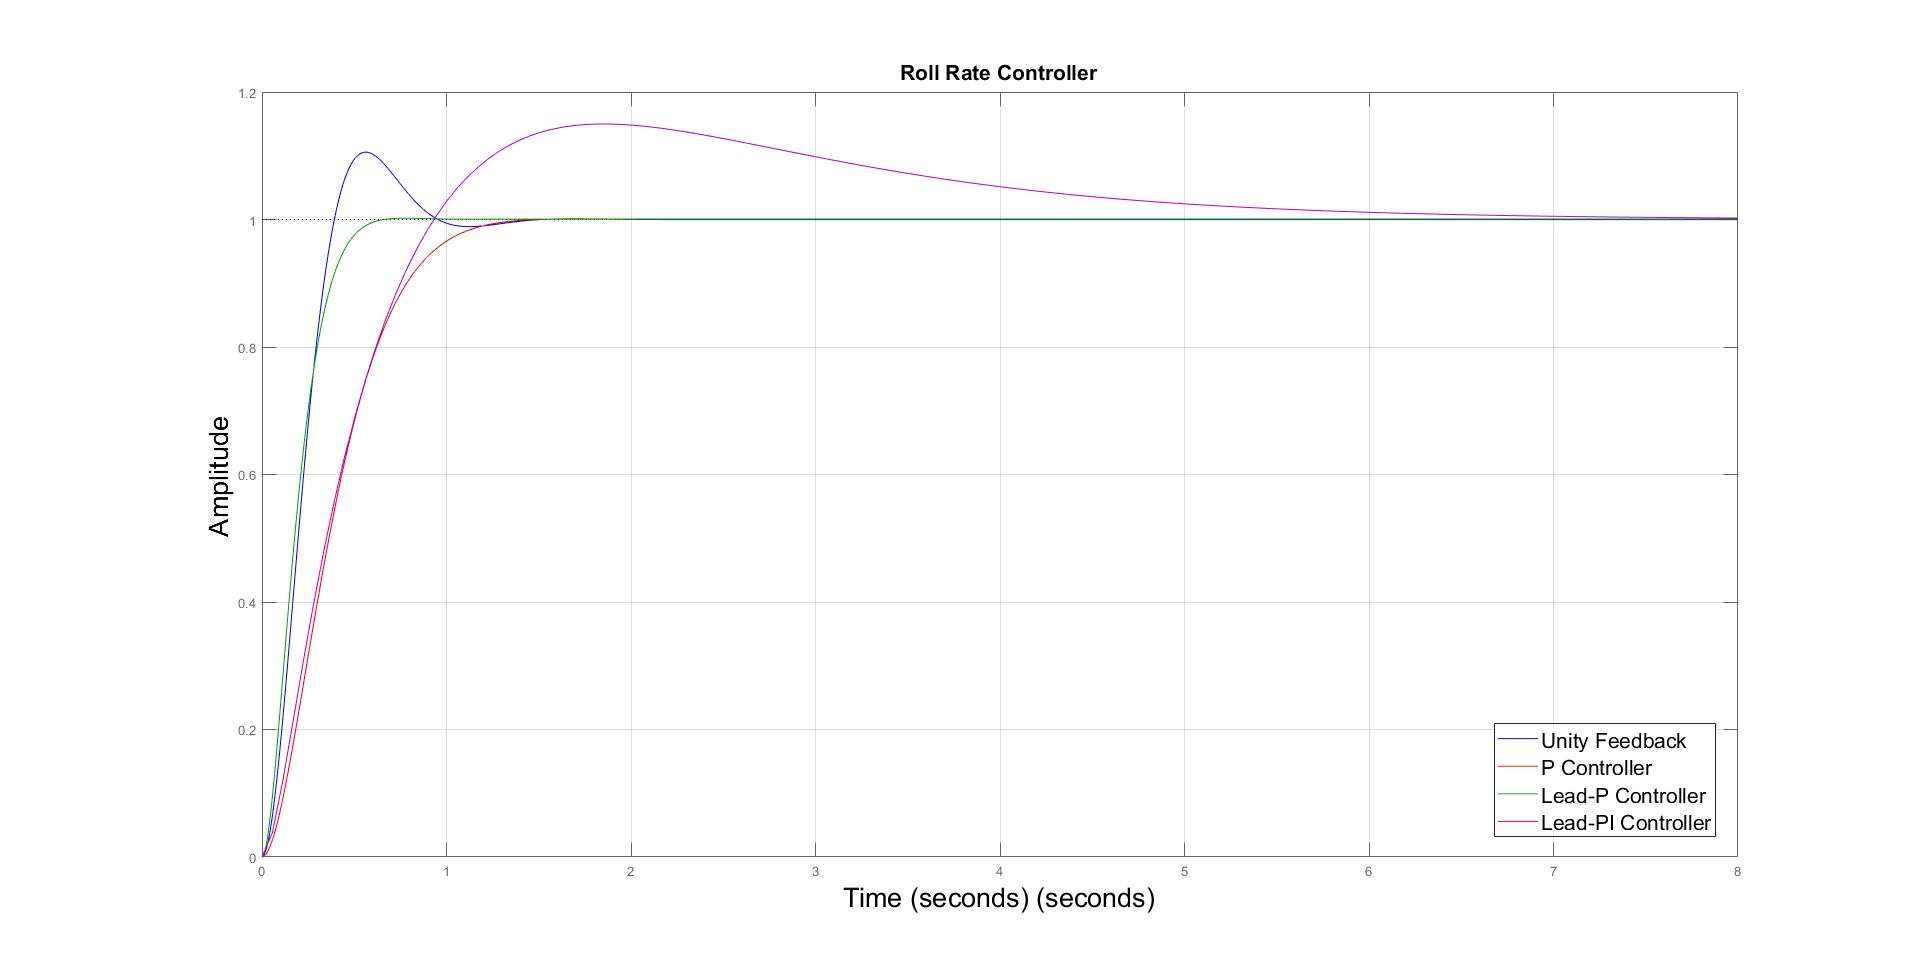
\includegraphics[height = 8cm]{../Design/Matlab/Controllers/roll_rate_step.jpg}
	\caption{Roll Rate Controller -  Step Responses}
	\label{IM_RollRateStep}
\end{figure}

The Lead-P controller has negligible overshoot and settles within $5$\,\% of the setpoint by $0.54$\,s. The integral term introduces more overshoot into the system, the unlimited Lead-PI system produces $13$\,\% overshoot and stretches the $5$\,\% settling time to $2$\,s. Limiting the integral term reduces the overshoot to $6$\,\% and the system now settles within $5$\,\% of the setpoint within $1.5$\,s. Although displaying distributed settling time, the standard deviation of rise times is only $25$\,ms.

\subsection{Pitch Rate Controller}	

\begin{figure}[H]
	\centering
	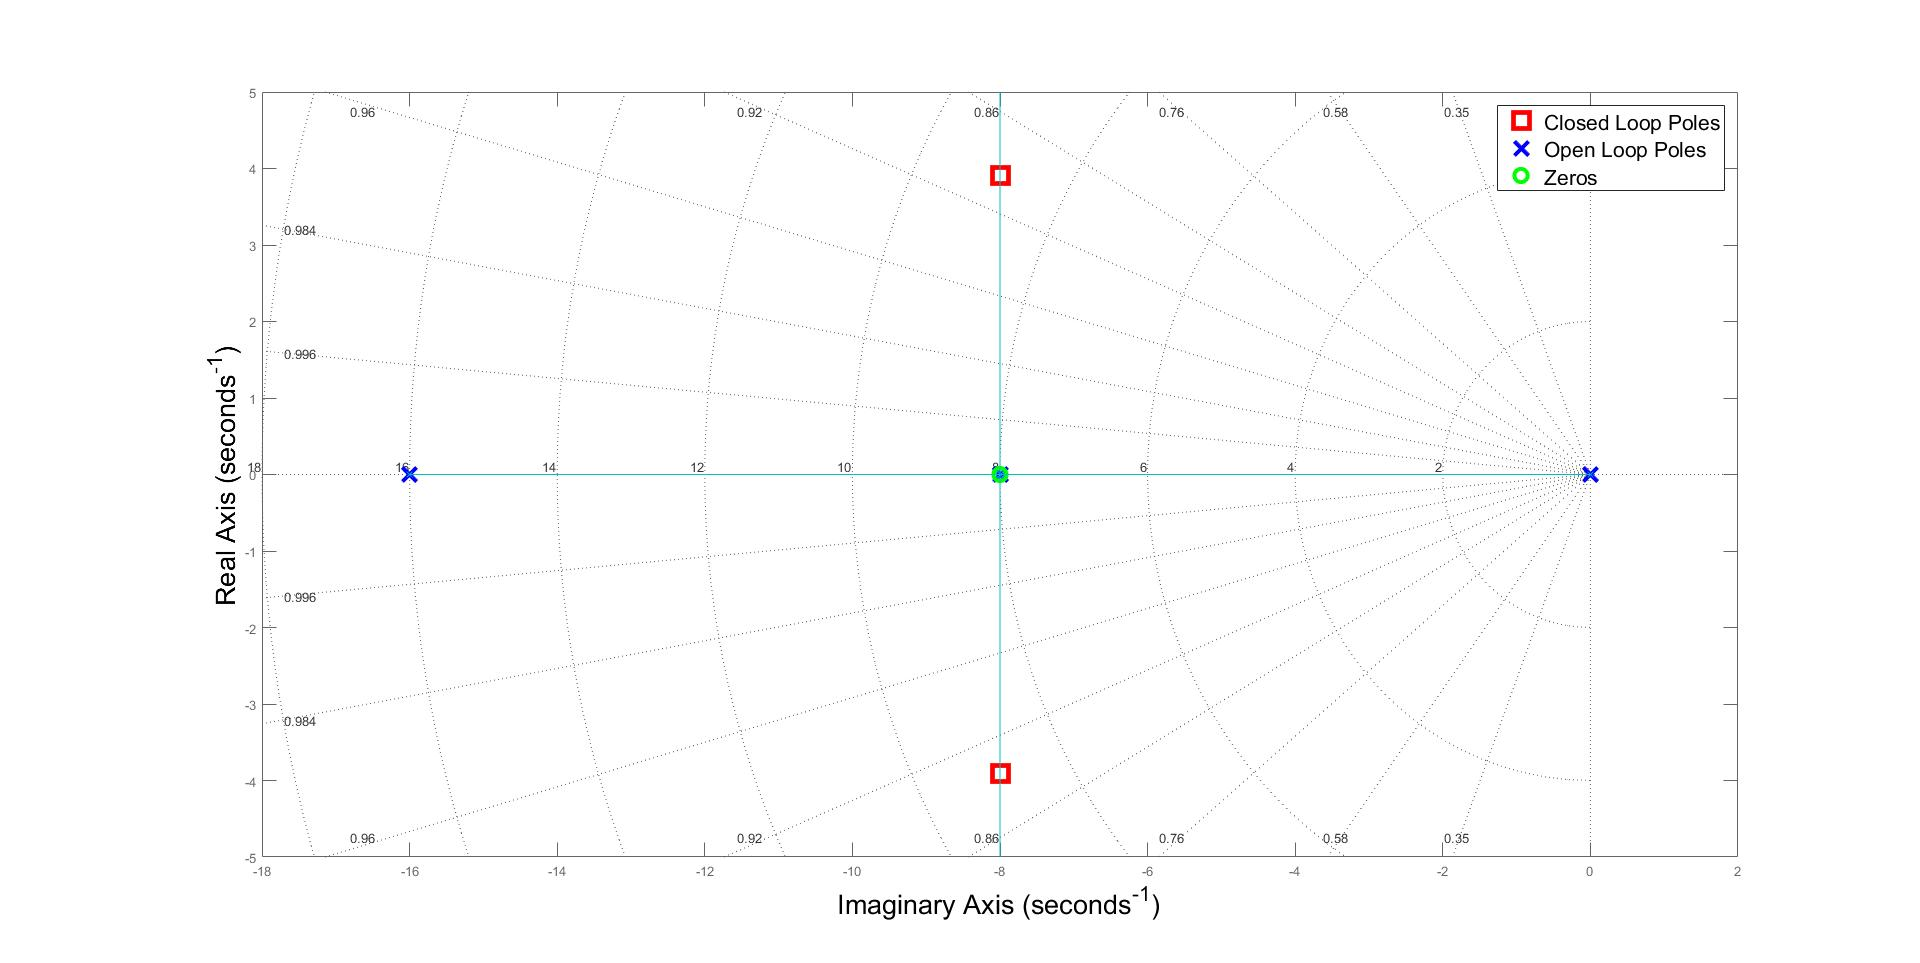
\includegraphics[height = 8cm]{../Design/Matlab/Controllers/pitch_rate_root.jpg}
	\caption{Pitch Controller -  Root Locus}
	\label{IM_PitchControlRoot}
\end{figure}

\begin{figure}[H]
	\centering
	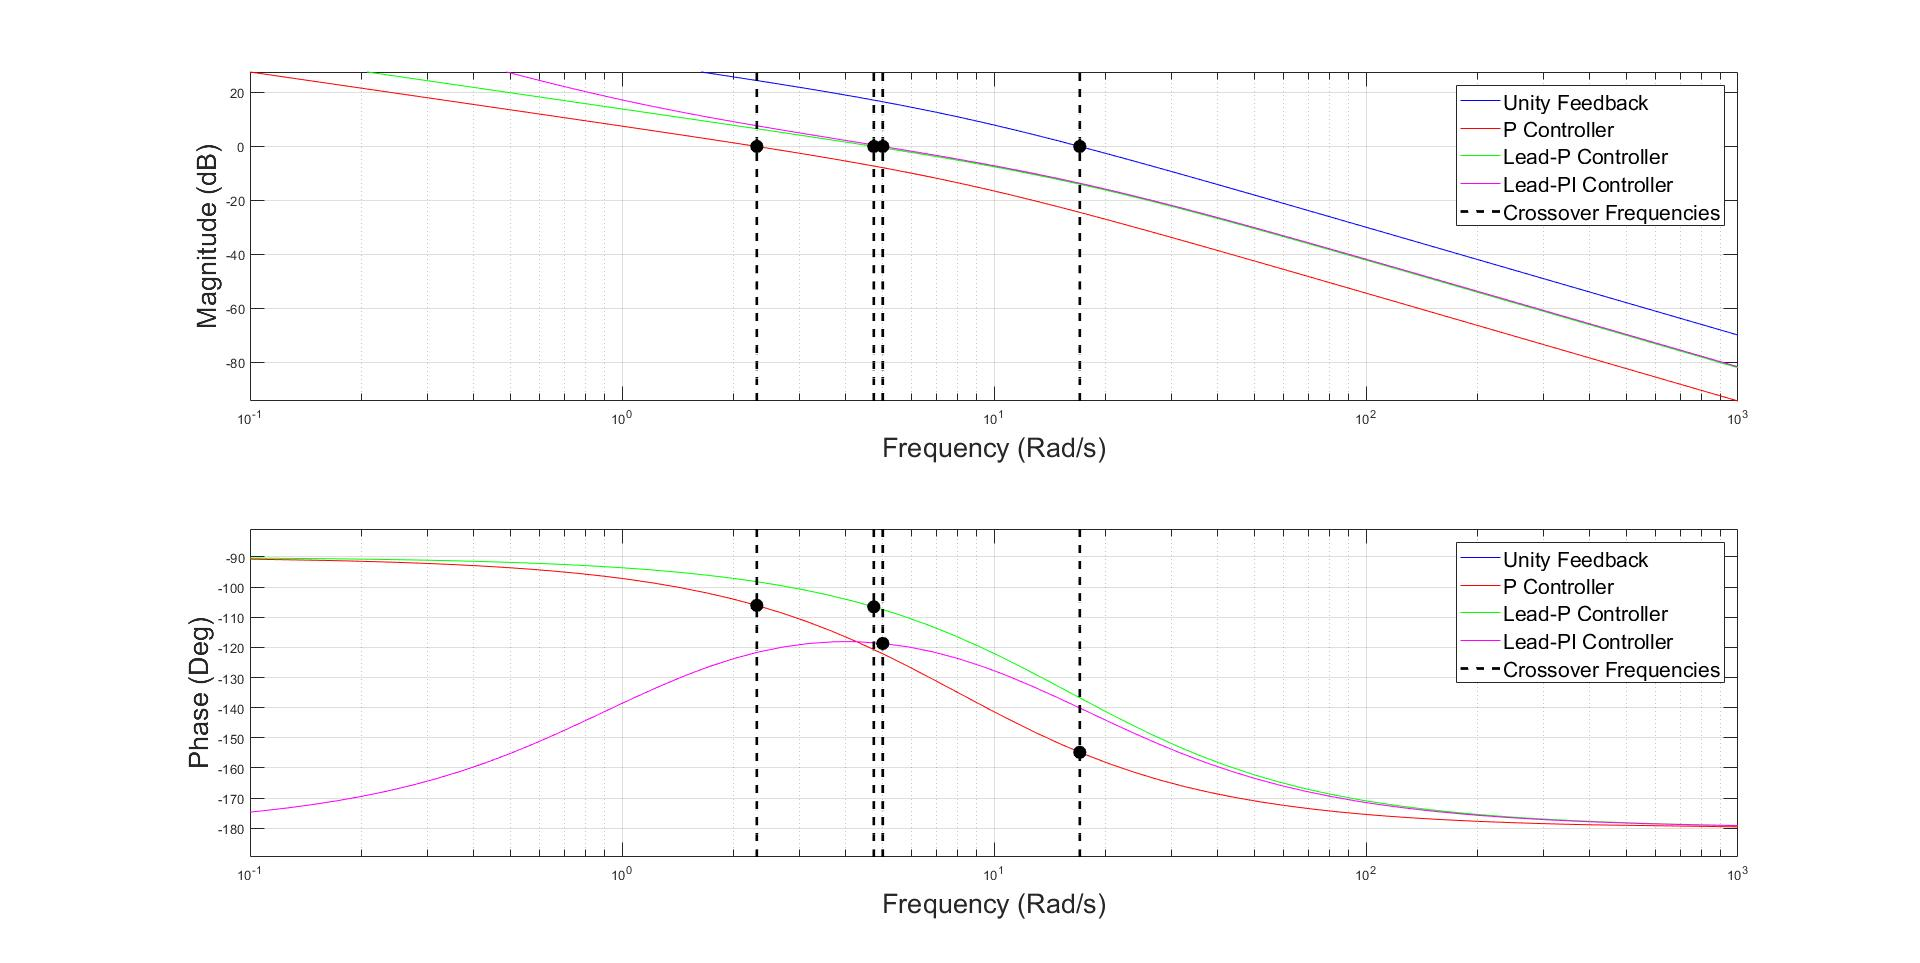
\includegraphics[height = 8cm]{../Design/Matlab/Controllers/pitch_rate_bode.jpg}
	\caption{Pitch Controller -  Bode Plots}
	\label{IM_PitchControlBode}
\end{figure}

\subsubsection{Pitch Rate Controller Discussion}

\begin{figure}[H]
	\centering
	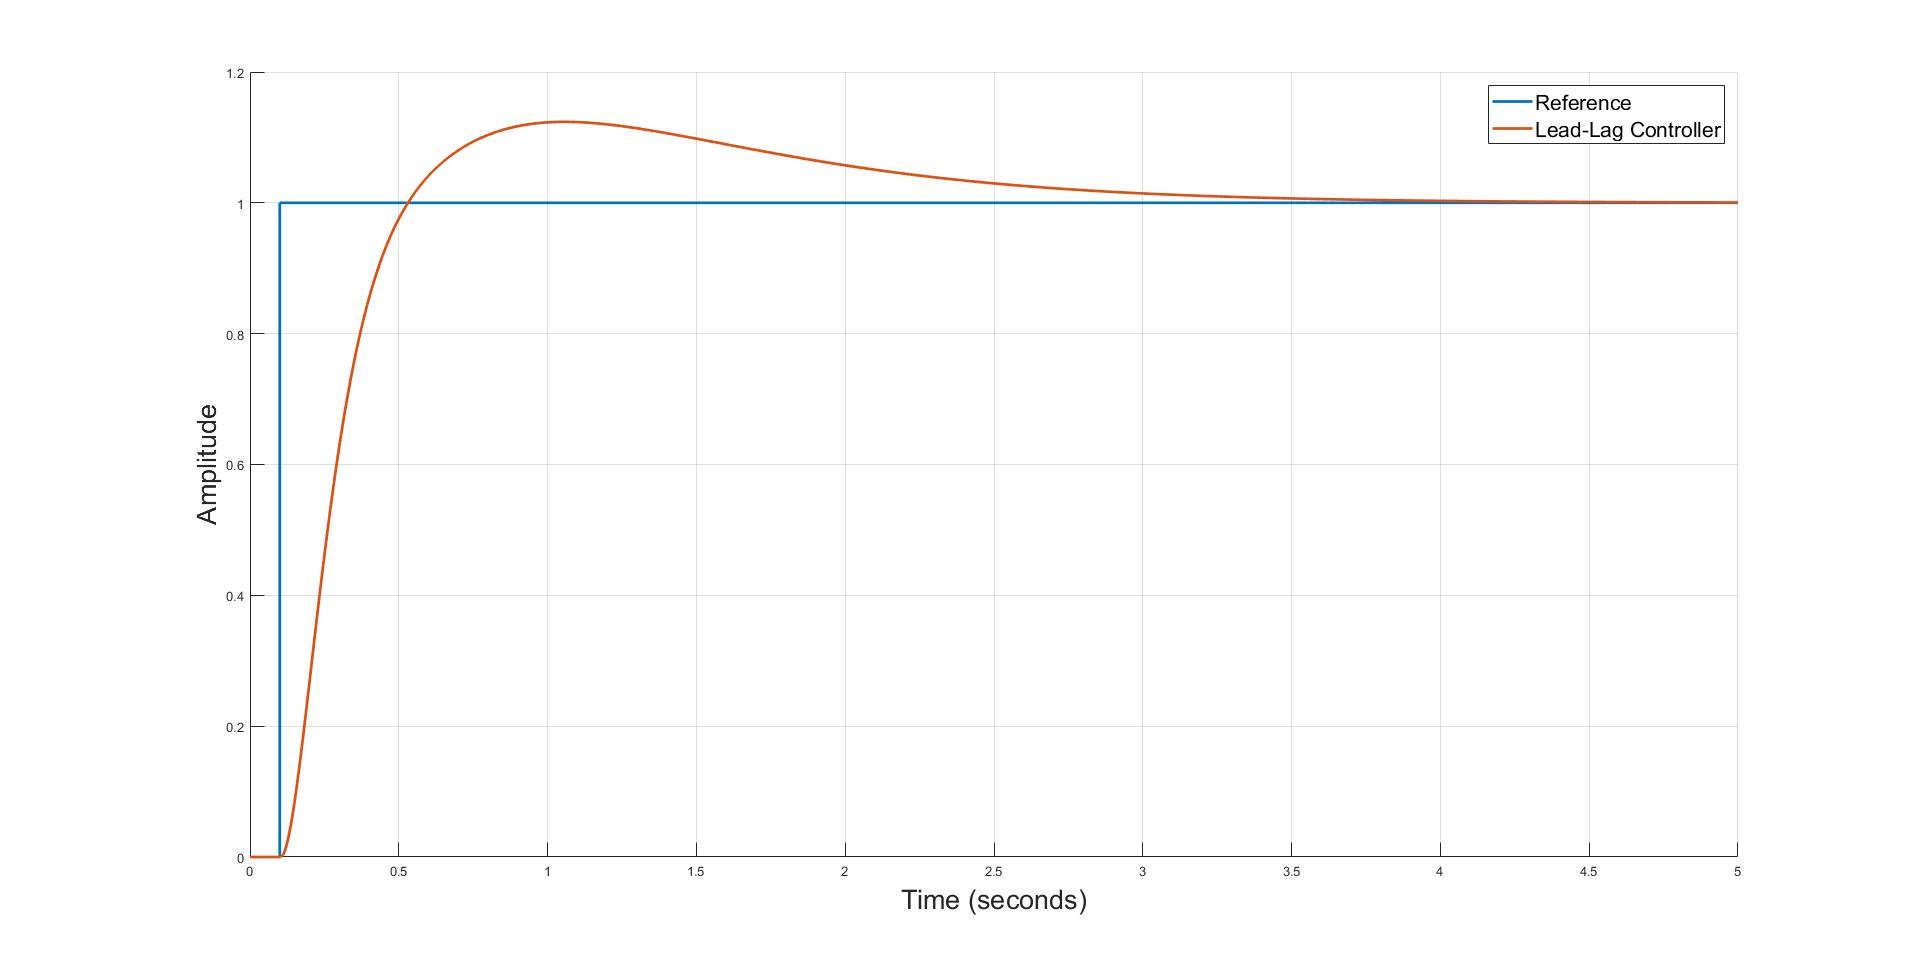
\includegraphics[height = 8cm]{../Design/Matlab/Controllers/pitch_rate_step.jpg}
	\caption{Pitch Rate Controller -  Step Responses}
	\label{IM_PitchRateStep}
\end{figure}



\begin{equation}
\label{EQ_PitchRateTF}
G(s) = \frac{\frac{1}{\tau I_{yy}}}{s (s + \frac{1}{\tau})}
\end{equation}


\subsection{Tilt Angle Controller}
The tilt angle controller is responsible for controlling the desired roll and pitch angles of the craft. The controller does this by commanding angular rates from a translational acceleration reference in the earth frame. Using the current angular position, this reference is converted to the body frame and used to calculate the error in angular positions for roll and pitch. This error is then fed through a Proportional gain. This section makes reference to Figure \ref{IM_TiltAngleController} and begins by explaining the method used for converting the acceleration reference into desired angular rates.

\begin{figure}[H]
	\centering
	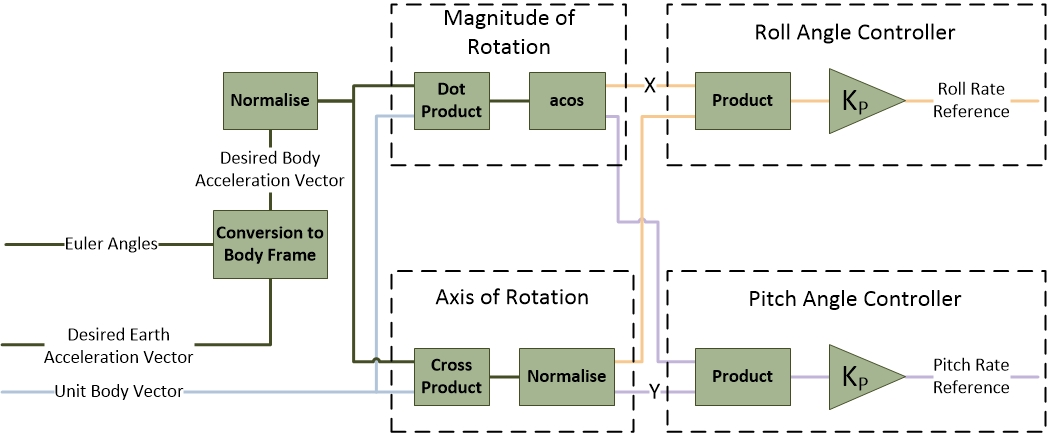
\includegraphics[height = 6.5cm]{../References/Diagrams/TiltAngleController.jpg}
	\caption{Tilt Angle Controller}
	\label{IM_TiltAngleController}
\end{figure}

\subsubsection{Method of Conversion}	
The first step to calculating the desired roll and pitch angles is to convert the earth frame set point into a body frame reference. The rotation matrix is calculated from the current Euler angles as seen in \eqref{EQ_RotationMatrix}.
The desired body acceleration vector is compared with a unit body vector. To remove any dependency on yaw, a unit Z body vector is created, which is perfectly aligned with the Z-Axis and thrust generation of the craft. Utilising the dot product shown in \eqref{EQ_DotProduct} the magnitude of the rotation can be calculated. Unit vectors are used, so simply taking the arc cosine of the result will produce the magnitude of rotation. The axis of rotation can be calculated by using the cross product shown in \eqref{EQ_CrossProduct} and normalising the output. Figure \ref{IM_AngleMethod} is used a visual aid for the preceding description.

\begin{equation}
\label{EQ_DotProduct}
\vec{a} \, \bigcdot \, \vec{b} = |ab|\,\cos \alpha
\end{equation}

\begin{equation}
\label{EQ_CrossProduct}
\vec{a} \, \times \, \vec{b} = \vec{c}
\end{equation}

\begin{figure}[H]
	\centering
	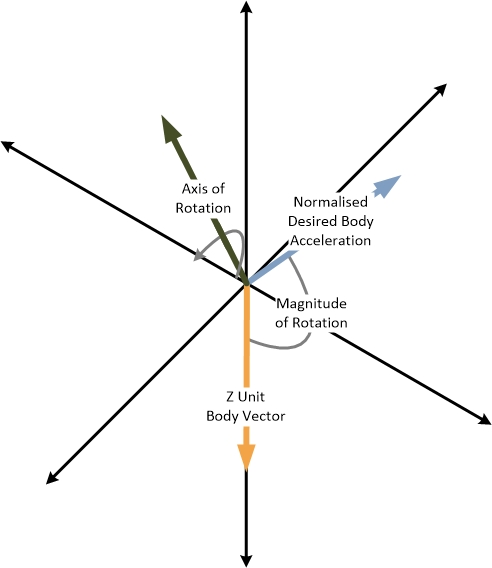
\includegraphics[height = 10cm]{../References/Diagrams/ConversionMethod.jpg}
	\caption{Conversion Technique using Dot and Cross Products}
	\label{IM_AngleMethod}
\end{figure}

\subsubsection{Roll Angle Controller}

\begin{figure}[H]
	\centering
	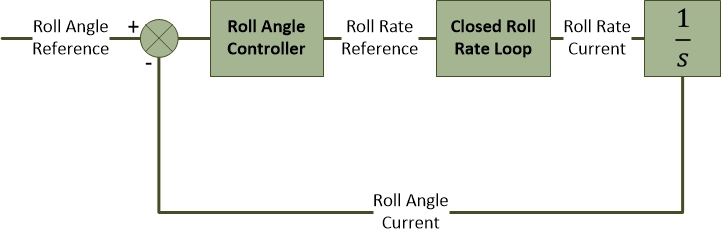
\includegraphics[height = 3.5cm]{../References/Diagrams/RollAngleLoop.jpg}
	\caption{Roll Angle Closed Loop}
	\label{IM_RollAngleLoop}
\end{figure}

\begin{figure}[H]
	\centering
	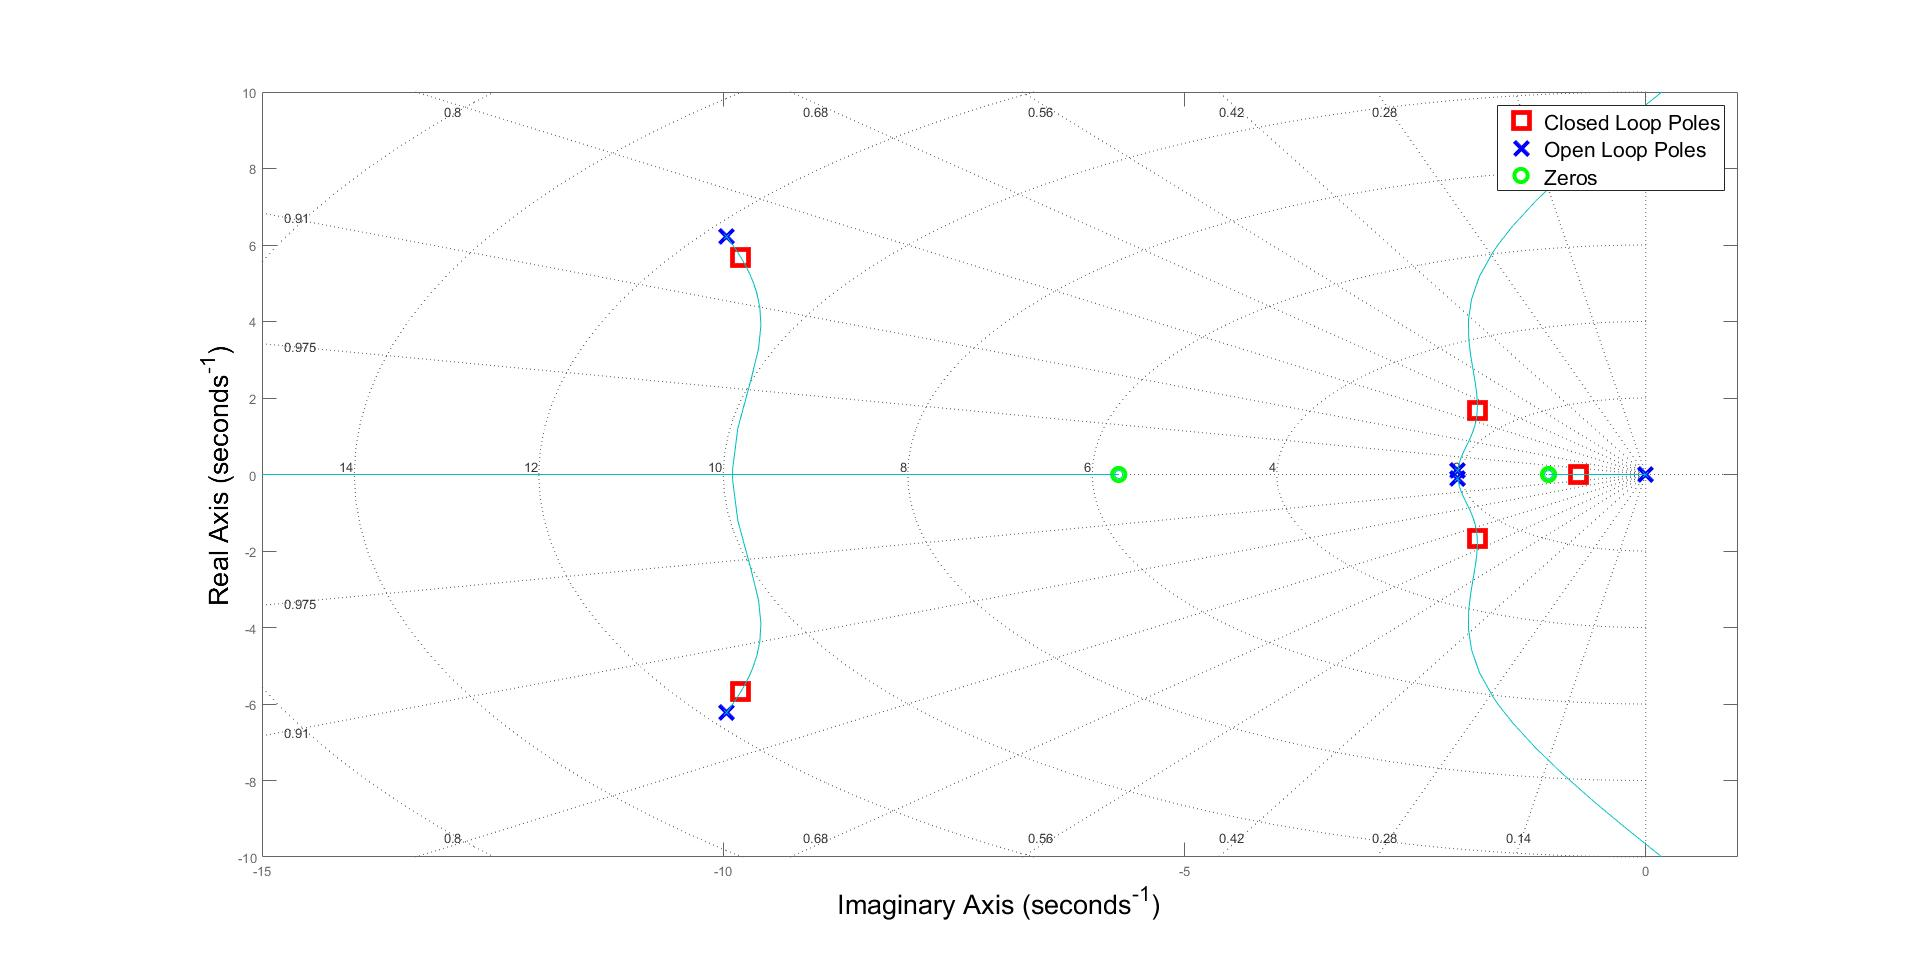
\includegraphics[height = 8cm]{../Design/Matlab/Controllers/roll_angle_root.jpg}
	\caption{Roll Angle Controller -  Root Locus}
	\label{IM_RollAngleControlRoot}
\end{figure}

\begin{figure}[H]
	\centering
	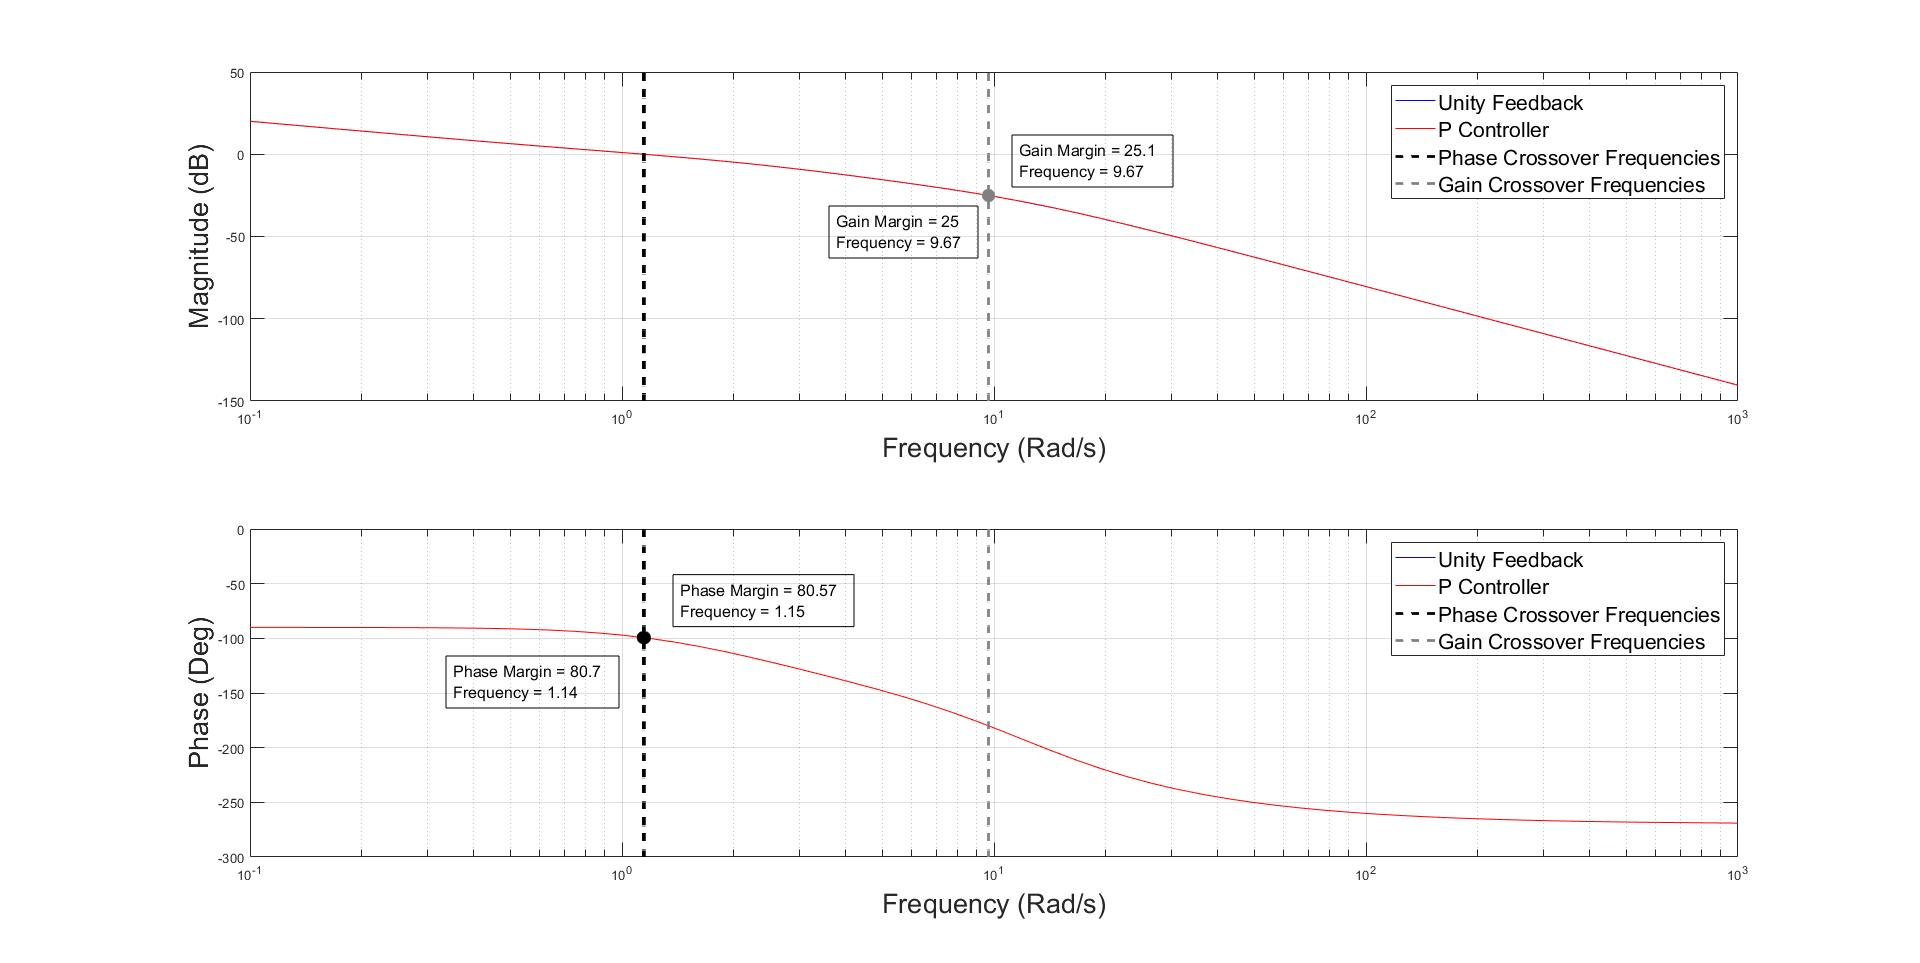
\includegraphics[height = 8cm]{../Design/Matlab/Controllers/roll_angle_bode.jpg}
	\caption{Roll Angle Controller -  Bode Plots}
	\label{IM_RollAngleControlBode}
\end{figure}


\begin{figure}[H]
	\centering
	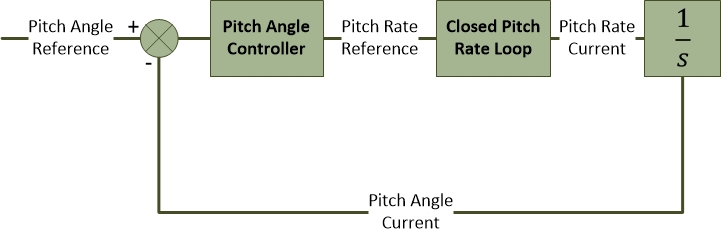
\includegraphics[height = 3.5cm]{../References/Diagrams/PitchAngleLoop.jpg}
	\caption{Pitch Angle Closed Loop}
	\label{IM_PitchAngleLoop}
\end{figure}

\begin{figure}[H]
	\centering
	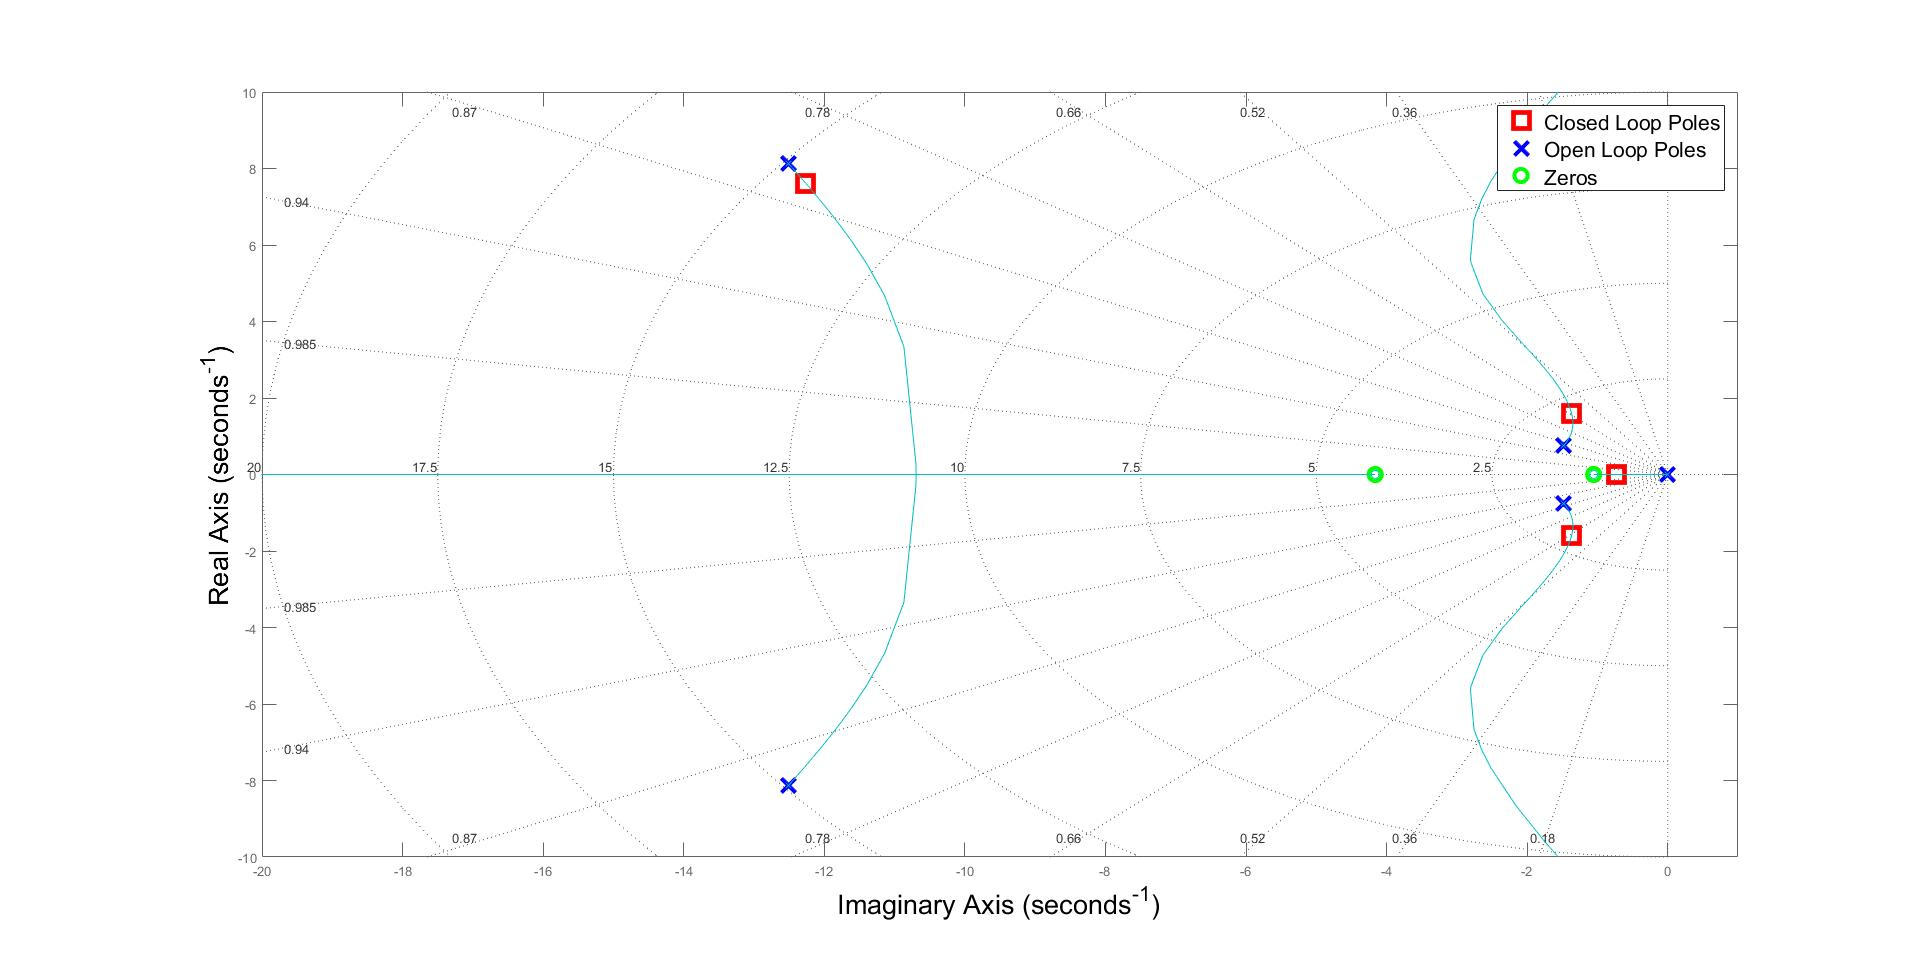
\includegraphics[height = 8cm]{../Design/Matlab/Controllers/pitch_angle_root.jpg}
	\caption{Pitch Angle Controller -  Root Locus}
	\label{IM_PitchAngleControlRoot}
\end{figure}

\begin{figure}[H]
	\centering
	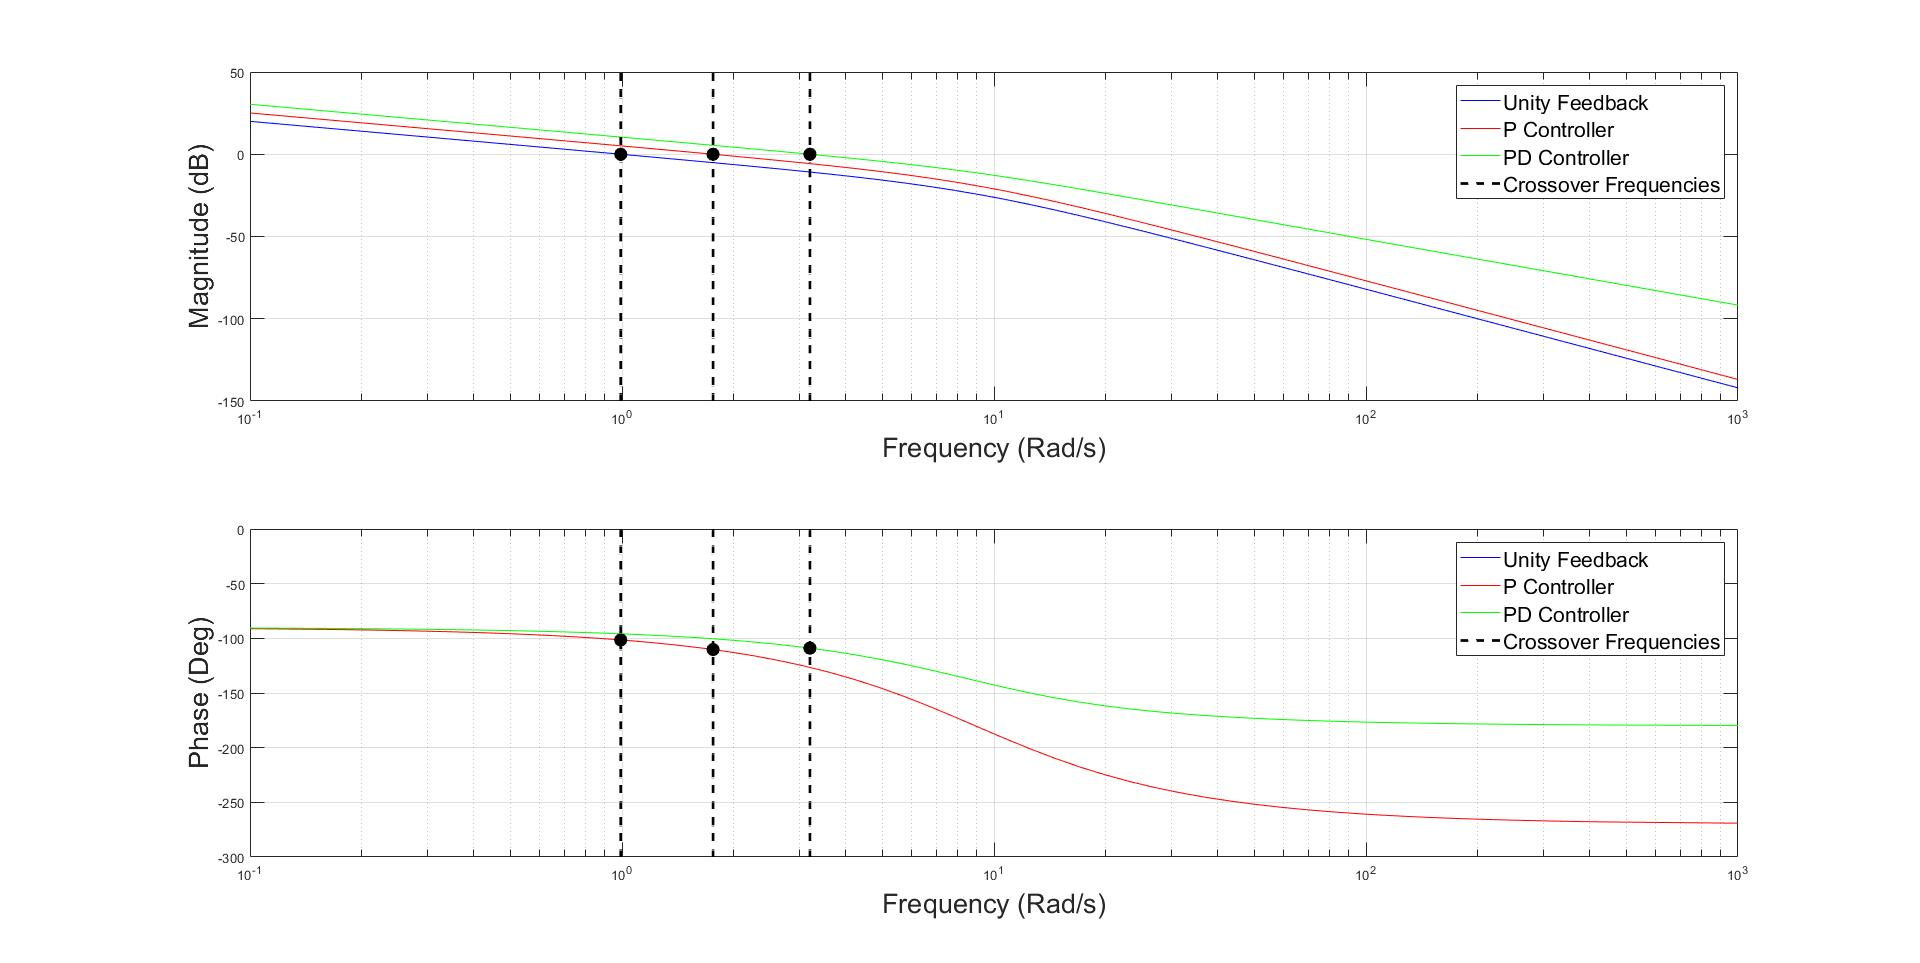
\includegraphics[height = 8cm]{../Design/Matlab/Controllers/pitch_angle_bode.jpg}
	\caption{Pitch Angle Controller -  Bode Plots}
	\label{IM_PitchAngleControlBode}
\end{figure}

\subsubsection{Tilt Angle Controller Discussion}

\begin{figure}[H]
	\centering
	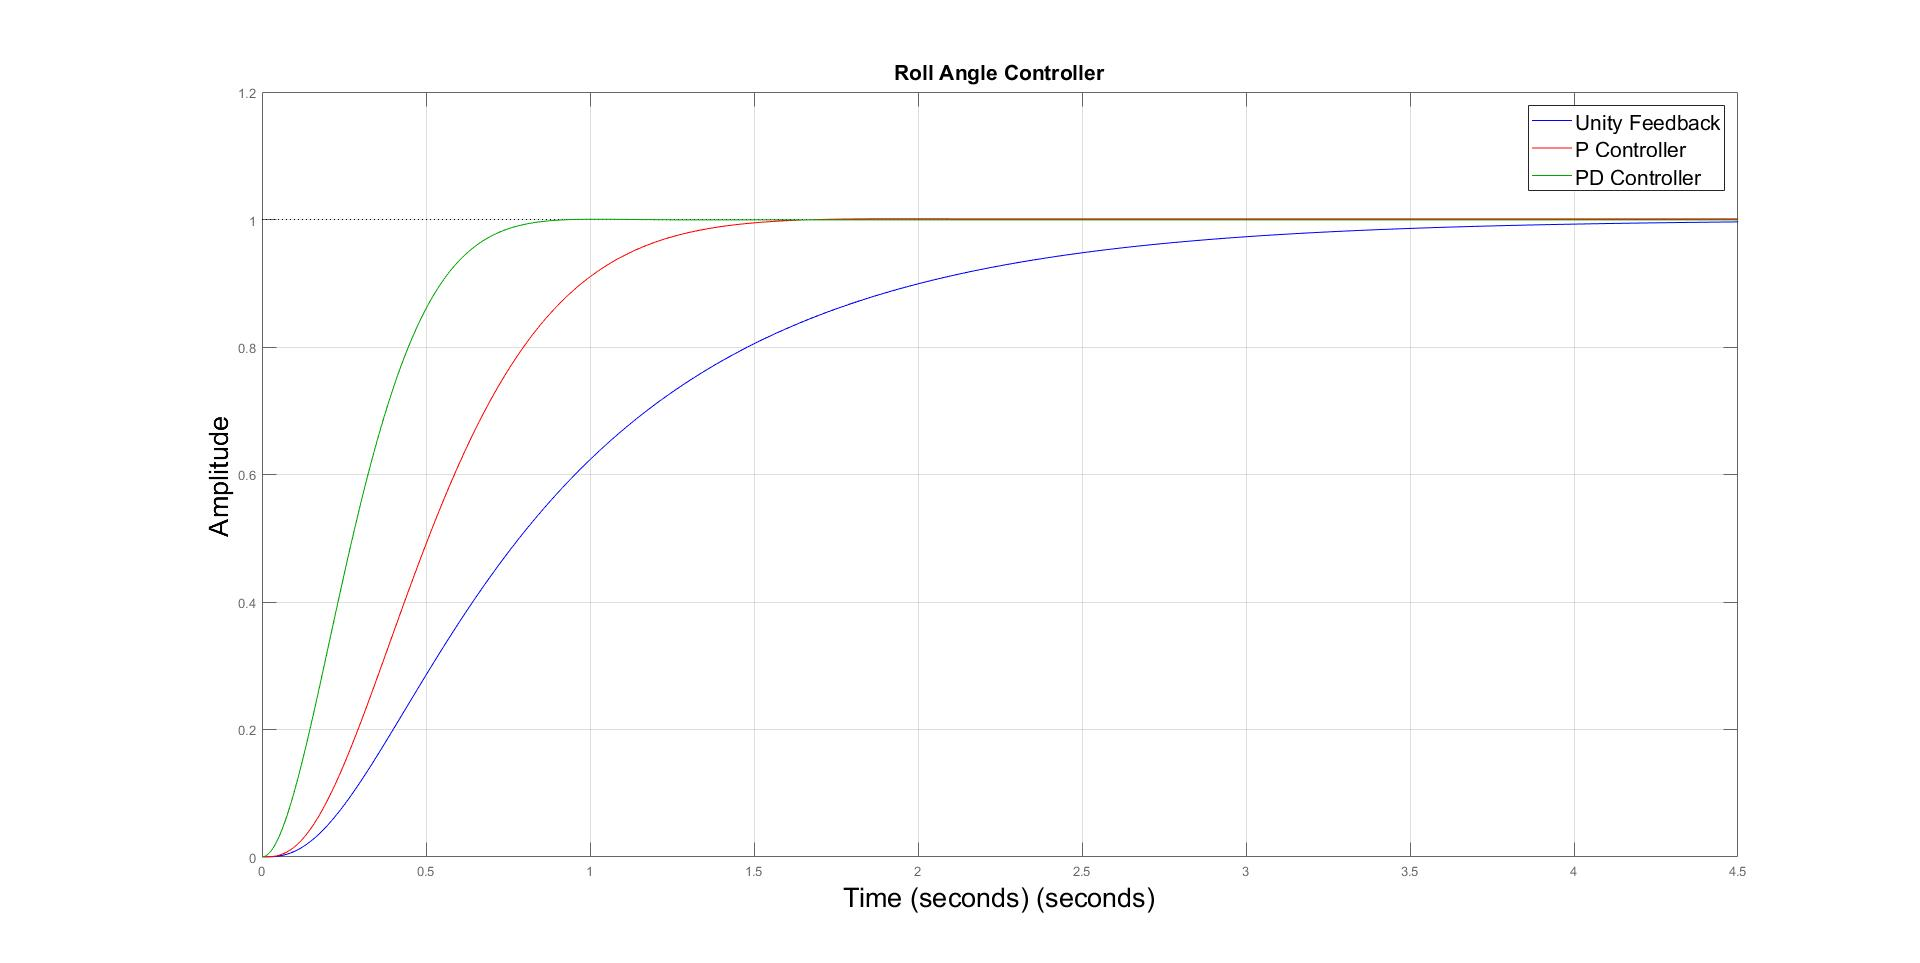
\includegraphics[height = 8cm]{../Design/Matlab/Controllers/roll_angle_step.jpg}
	\caption{Roll Angle Controller -  Step Responses}
	\label{IM_RollAngleStep}
\end{figure}

\begin{equation}
\label{EQ_RollAngleTF}
G(s) = \frac{\frac{1}{\tau I_{zz}}}{s (s + \frac{1}{\tau})}
\end{equation}


\subsection{Linear Velocity Control}

\subsection{Global Position Tracking Control}

\section{Heading Controller}
This section describes the heading controller which is responsible for aligning the craft with a desired yaw angle reference. An angle reference is given to a yaw angle controller which outputs a yaw rate reference. The inner yaw rate controller commands the yawing moment around the Z-Axis of the craft. Both the vertical and the horizontal controllers have been designed to operate independently of the heading. The craft is however, expected to fly down a narrow channel. This calls for a method of aligning the body axis of the craft with a given heading in the earth frame. This heading could be given by a higher flight planning strategy.

The craft must be able to follow a heading setpoint with zero steady state error and have a reasonably damped response \todo[inline]{to vague?}. The heading controller must also be able to reject disturbances and will require an integrator in the control law. The yaw controller must also consider that the yaw torque generation has a reduction gain due to the lift to drag ratio. The design of the craft also means the yaw rate dynamics produce the lowest plant gain with the largest inertia component. The juxtaposition of a low actuation torque and lower plant gain leads to the heading controller typically being slower and exhibit less bandwidth when compared to the other controllers. Before a controller can be designed, the plant dynamics must be derived.

\subsection{Yaw Rate Dynamics}
Using Newton mechanics at near hover conditions, the yaw dynamics for the craft can be derived, the result is shown in equation \eqref{EQ_YawNewton}. $\dot{r}$ is the rotational acceleration of the craft and $N$ is the instantaneous moment experienced by the craft around the Z-Axis.

\begin{equation}
\label{EQ_YawNewton}
\dot{r} = \dfrac{N}{I_{ZZ}}
\end{equation}

$\dot{r}$ is chosen as the output of the system with the state variable chosen as $N$. From this, the space equation for the system can be derived and is shown in \eqref{EQ_YawStateSpace1} and \eqref{EQ_YawStateSpace2}. 

\begin{eqnarray}
[\dot{N}] &=& - [\dfrac{1}{\tau}] \ [N] + [\dfrac{1}{\tau}] [\delta_\psi]\label{EQ_YawStateSpace1}\\\label{EQ_HeaveStateSpace22}
[\dot{r}] &=& - [\dfrac{1}{I_{ZZ}}] \ [N]\label{EQ_YawStateSpace2}\\
G(s)_{yaw} &=& \frac{\frac{1}{\tau I_{ZZ}}}{s (s + \frac{1}{\tau})}\label{EQ_YawTF}
\end{eqnarray}

From the state space representation, the transfer function for the yaw acceleration can be calculated. Integrating the result produces the transfer function for yaw rate, introducing a new pole into the system, the result is shown in \eqref{EQ_YawTF}. This plant now has two open loop poles, the first pole is due to the lag introduced by the motor rotor system, and lies at $\sigma = -\dfrac{1}{\tau} = 8$ with the second due to the integration of yaw acceleration to velocity. 

\subsection{Yaw Rate Controller}	
The yaw rate controller receives a yaw acceleration reference in radians per second (rad/s) and outputs the virtual actuator $\sigma_{\psi}$. The yawing moment is generated by air pressure on the rotors as they generate thrust, the reduction gain introduces the possibility of saturating the other controllers for large step inputs. However, as the most inner of the two heading loops, the yaw rate system limits the bandwidth of the outer yaw angle loop. The yaw rate controller must then produce enough bandwidth for the yaw angle controller, while ensuring it is not commanding thrust values above the limits described in \ref{tab:HeadRoomPercentages}. The yawing moment torque generation is also less accurately modelled \todo[inline]{better way of saying this? Trying to say that it is harder to accurately measure and is more susceptible for modelling errors} and the system must exhibit high stability with large gain and phase margins. The free integrator in the yaw rate system will produce zero steady state error. The design for this controller can then be designed as a simple P controller with a non-linear saturation as shown in Figure \ref{IM_YawRateController}.

\begin{figure}[H]
	\centering
	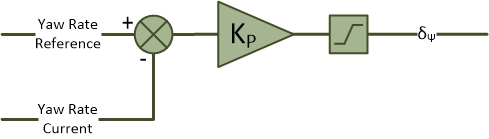
\includegraphics[height = 3.5cm]{../References/Diagrams/YawRateController.jpg}
	\caption{Yaw Rate Controller -  Control Diagram}
	\label{IM_YawRateController}
\end{figure}

The dynamic response of the proportional (P) controller is evaluated using the root locus in Figure \ref{IM_YawRateControlRoot}. The controller adds no new poles or zeros. The proportional gain is used to move the closed loops and achieve the desired bandwidth. The final closed loops poles sit at $-4 \pm 1.93$\,rad/s, the poles are slightly under damped with a damping ratio of $0.9$.

\begin{figure}[H]
	\centering
	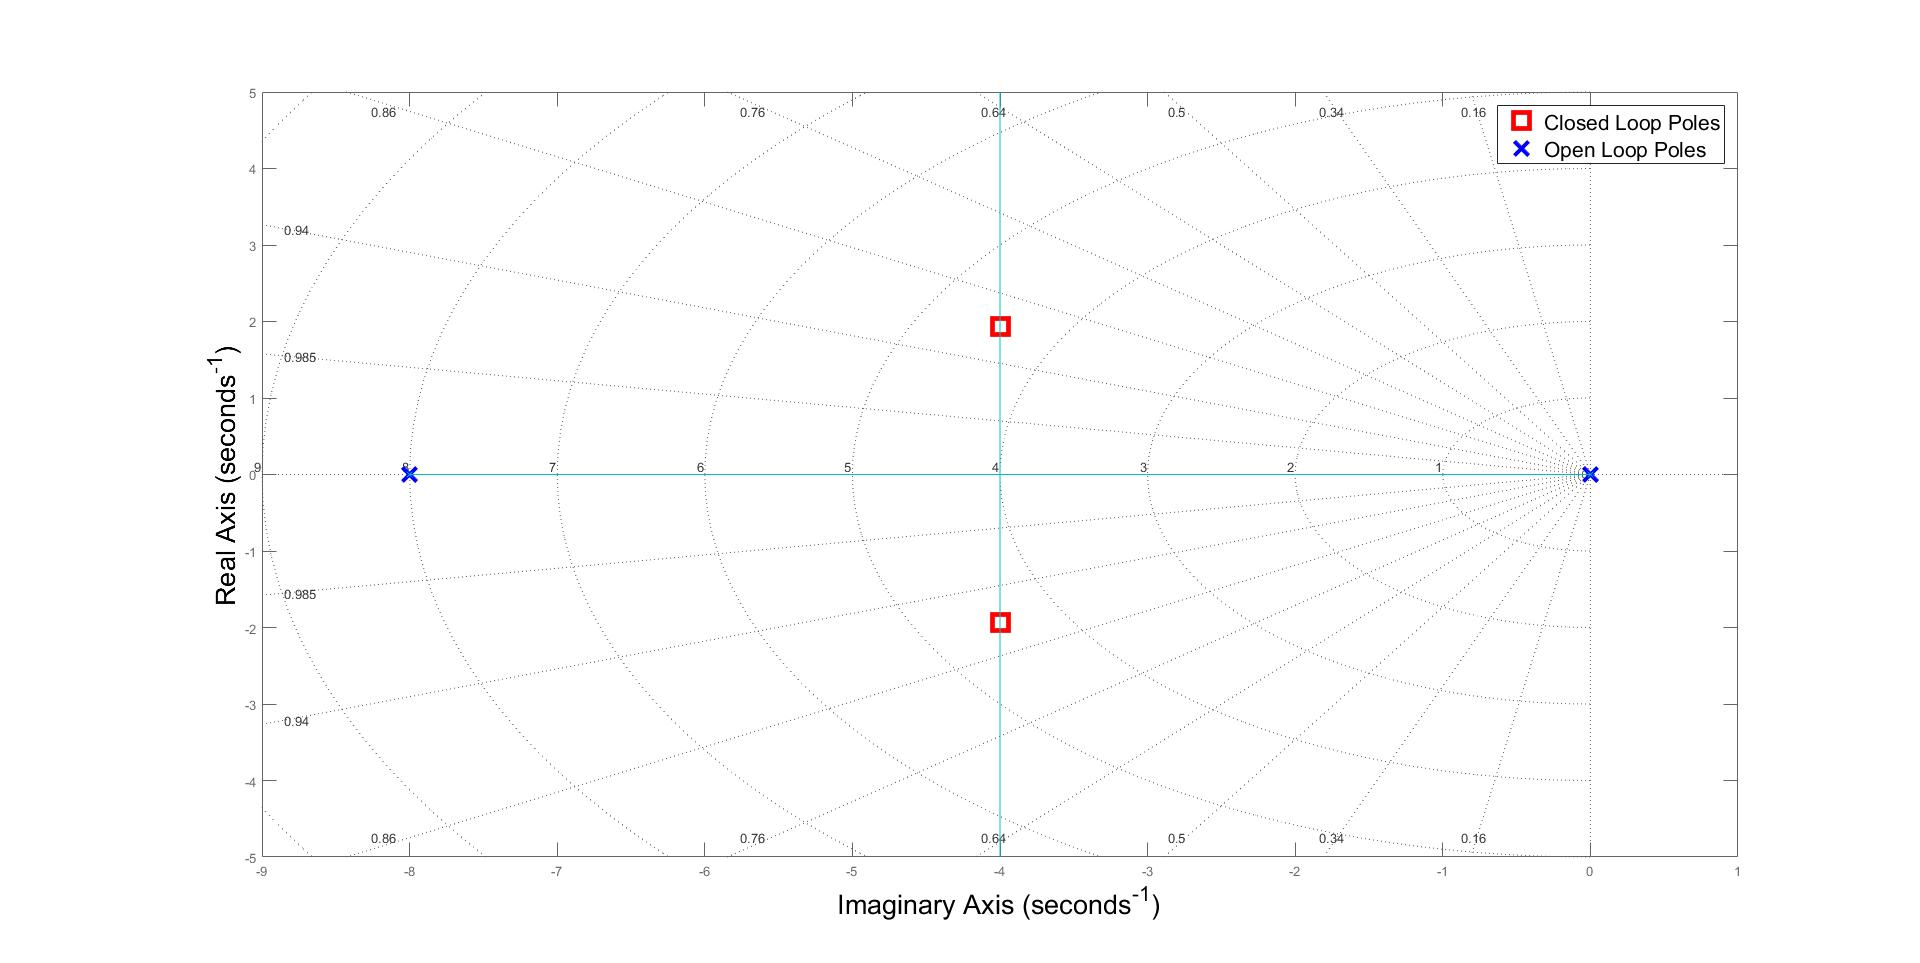
\includegraphics[height = 8cm]{../Design/Matlab/Controllers/yaw_rate_root.jpg}
	\caption{Yaw Rate Controller -  Root Locus}
	\label{IM_YawRateControlRoot}
\end{figure}

The bode plot in Figure \ref{IM_YawRateControlBode} is used to evaluate the frequency response of the system against unity feedback. As expected the controller introduces no phase change into the system. Unity feedback produces a crossover frequency of $4.99$\,rad/s which is too fast for the heading system. Reducing the gain of the system increases the phase margin to $74$\textdegree and reduces the crossover frequency by nearly half to $2.37$\,rad/s.

\begin{figure}[H]
	\centering
	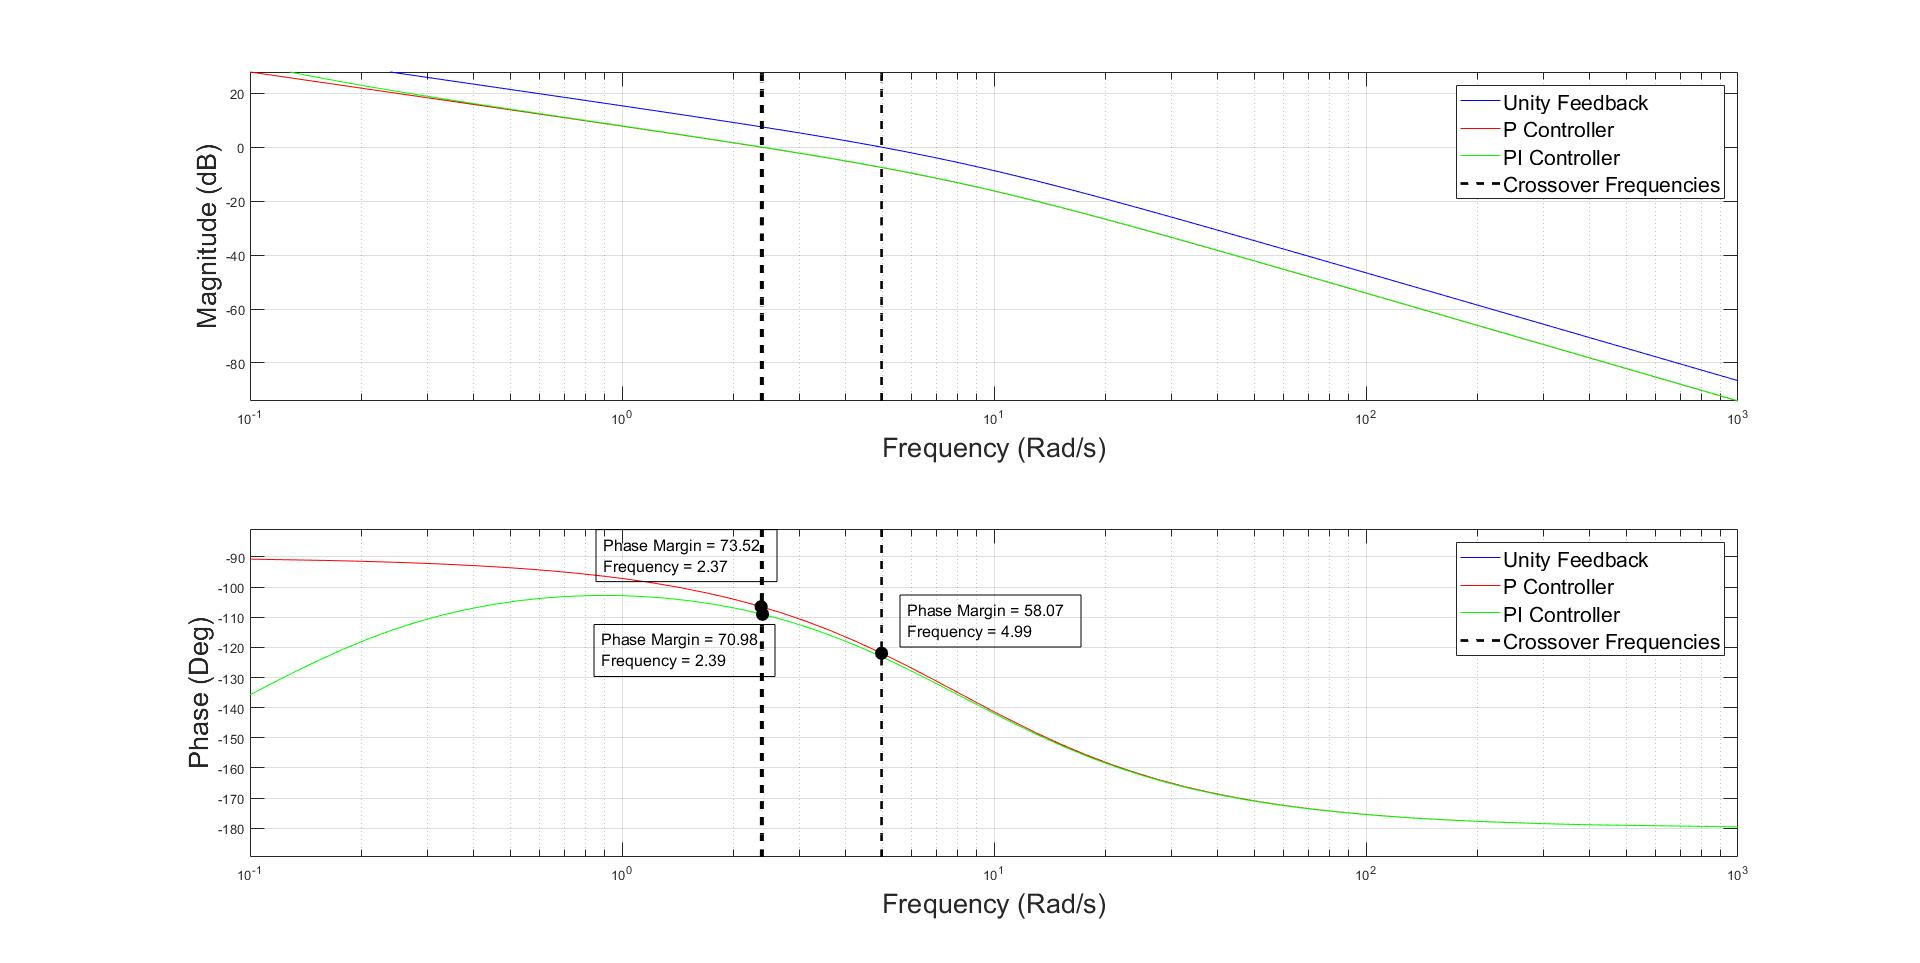
\includegraphics[height = 8cm]{../Design/Matlab/Controllers/yaw_rate_bode.jpg}
	\caption{Yaw Rate Controller -  Bode Plots}
	\label{IM_YawRateControlBode}
\end{figure}

\subsubsection{Yaw Rate Controller Discussion}
The controller increases stability in the system and produces the step response shown in Figure \ref{IM_YawRateStep}. The system has a $5\% $ settling time of $0.9s$ and negligible overshoot. The maximum thrust commanded per motor using this system is $0.26$\,N, which falls in the limits of this system. The low gain of the system makes this system susceptible to disturbances and calls for an outer angle loop. 

\begin{figure}[H]
	\centering
	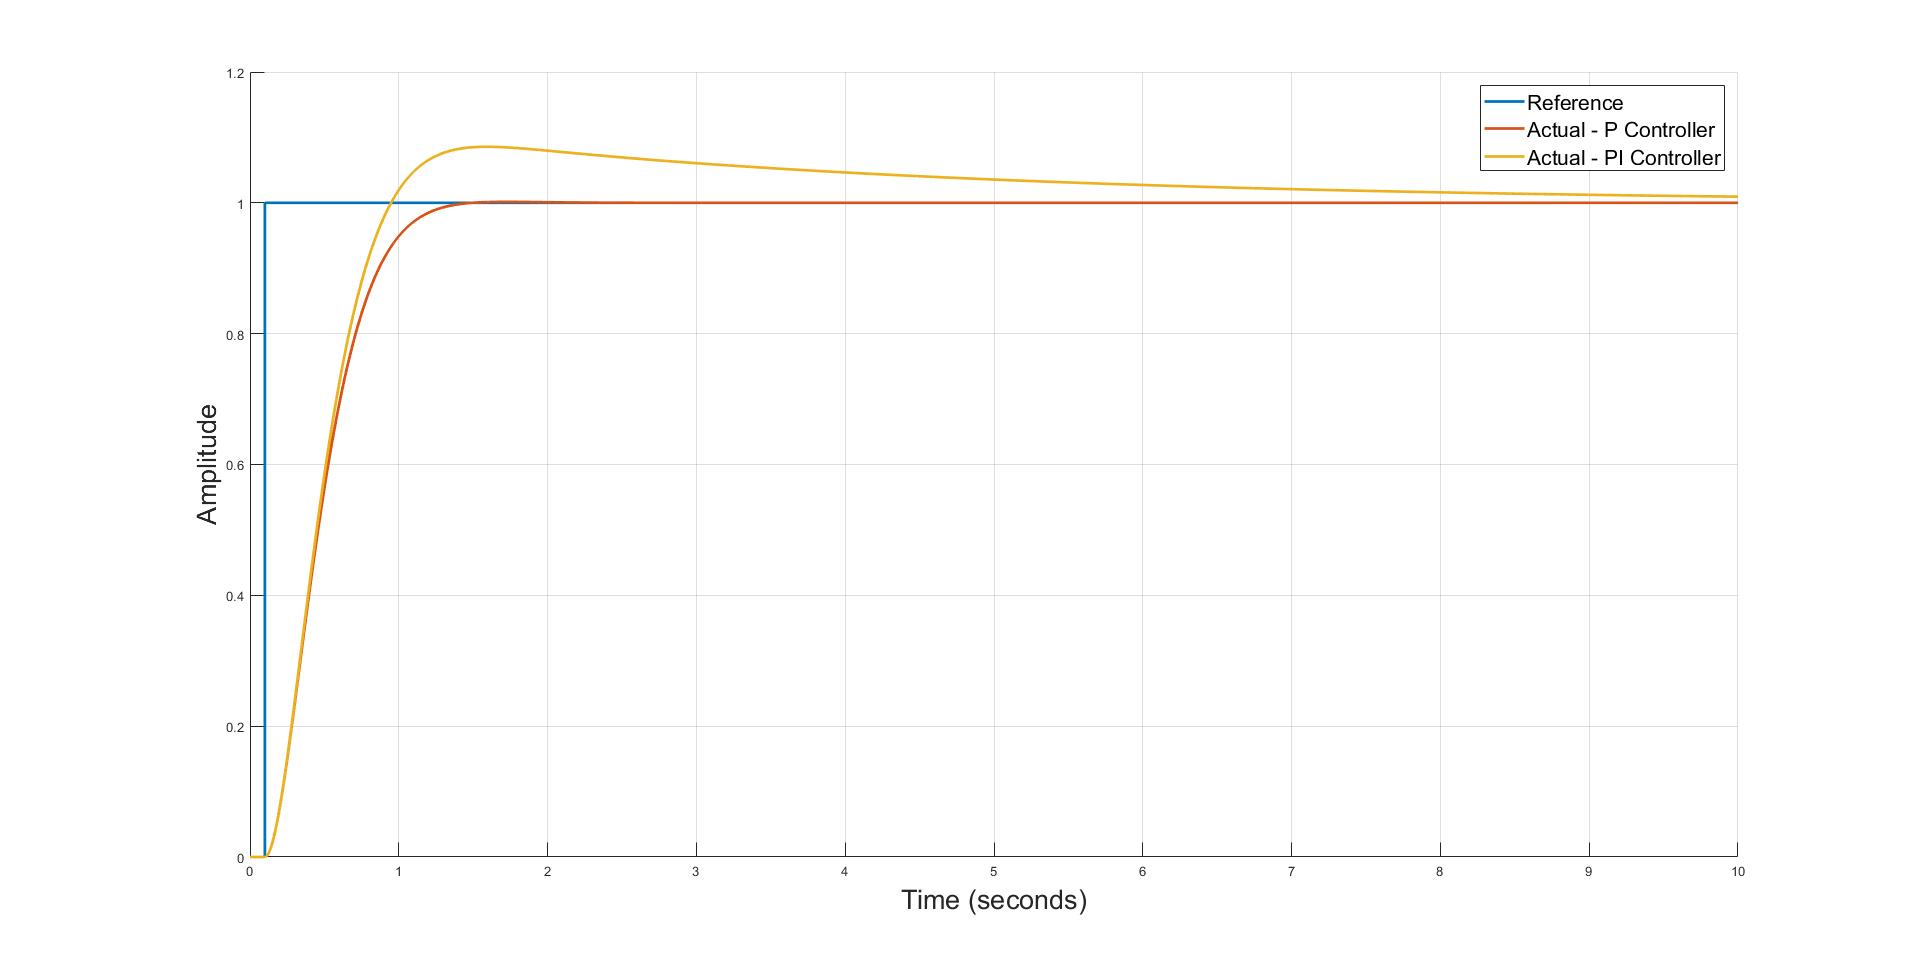
\includegraphics[height = 8cm]{../Design/Matlab/Controllers/yaw_rate_step.jpg}
	\caption{Yaw Rate Controller -  Step Responses}
	\label{IM_YawRateStep}
\end{figure}

\subsection{Yaw Angle Controller}	
The yaw angle controller receives a heading reference in radians and outputs a yaw angle rate reference in radians per second to the inner rate controller as shown in Figure \ref{IM_YawAngleLoop}. This controller is limited by the inner loop and must ensure significant bandwidth between the inner and outer loops. The system must be able to reject disturbances and requires an integrator in the system. The system must be reasonably damped \todo[inline]{Too Vague?} with limited overshoot.

\begin{figure}[H]
	\centering
	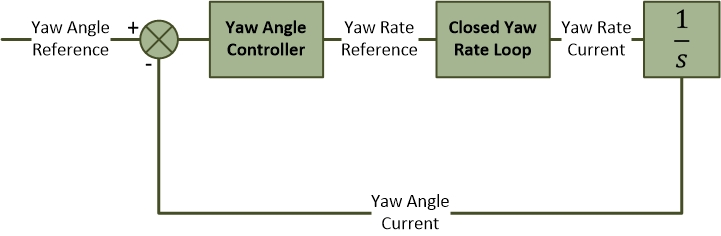
\includegraphics[height = 3.5cm]{../References/Diagrams/YawAngleLoop.jpg}
	\caption{Yaw Angle PI Controller -  Control Diagram}
	\label{IM_YawAngleLoop}
\end{figure}

Initially a Proportional Integral (PI) controller was considered as shown in Figure \ref{IM_YawAngleController}. The proportional gain is used to move the closed loop poles and achieve the desired bandwidth. The integral term is introduced to account for expected disturbances as well as measurement errors in the rate loop. The PI controller adds a new zero and a new pole into the system. 

\begin{figure}[H]
	\centering
	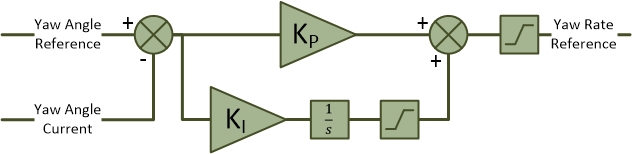
\includegraphics[height = 3.5cm]{../References/Diagrams/YawAngleControllerPI.jpg}
	\caption{Yaw Angle PI Controller -  Control Diagram}
	\label{IM_YawAngleController}
\end{figure}

The second scheme was designed as a Proportional Integral Derivative (PID) controller as shown in Figure \ref{IM_YawAngleControllerPID}, the differential term is introduced to increase the phase of the system and adds an additional zero. The differential command is fed through a low pass filter to reduce noise on the command. As shown both controllers contain non linear elements that are not considered during the linear design. The components excluded during the analysis are all the limiters as well as the low pass filter seen in the differentiator portion of the PID leg.

\begin{figure}[H]
	\centering
	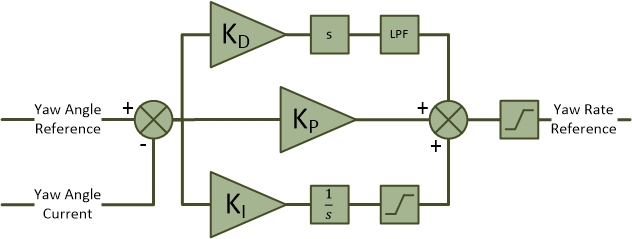
\includegraphics[height = 5.5cm]{../References/Diagrams/YawAngleControllerPID.jpg}
	\caption{Yaw Angle PID Controller -  Control Diagram}
	\label{IM_YawAngleControllerPID}
\end{figure}

The dynamic response of each system can be evaluated using the root loci diagrams seen in Figure \ref{IM_YawAngleControlRoot}. The plant has two open loop poles at the closed loop yaw rate pole locations, as well as a new pole at the origin introduced by the mathematical relationship between speed and position. Both controllers introduce one new open loop pole at the origin and at least one zero. The PID controller introduces an additional zero into the system.  

The final closed loop pole positions for the PI controller all lie on the imaginary axis and are located at $-3.62$, $-3.26$, $-0.88$ and $-0.25$. The PID controller has a dominant complex pair of closed loop poles at $-0.52 \pm 0.51 i$ with the other non-dominant closed loop pole pair sitting at $-3.48 \pm 2.54 i$. The PI controller has critically damped dominant poles where as the dominant poles for the PID controller are under damped with a damping ratio of $0.71$.

\begin{figure}[H]
	\centering
	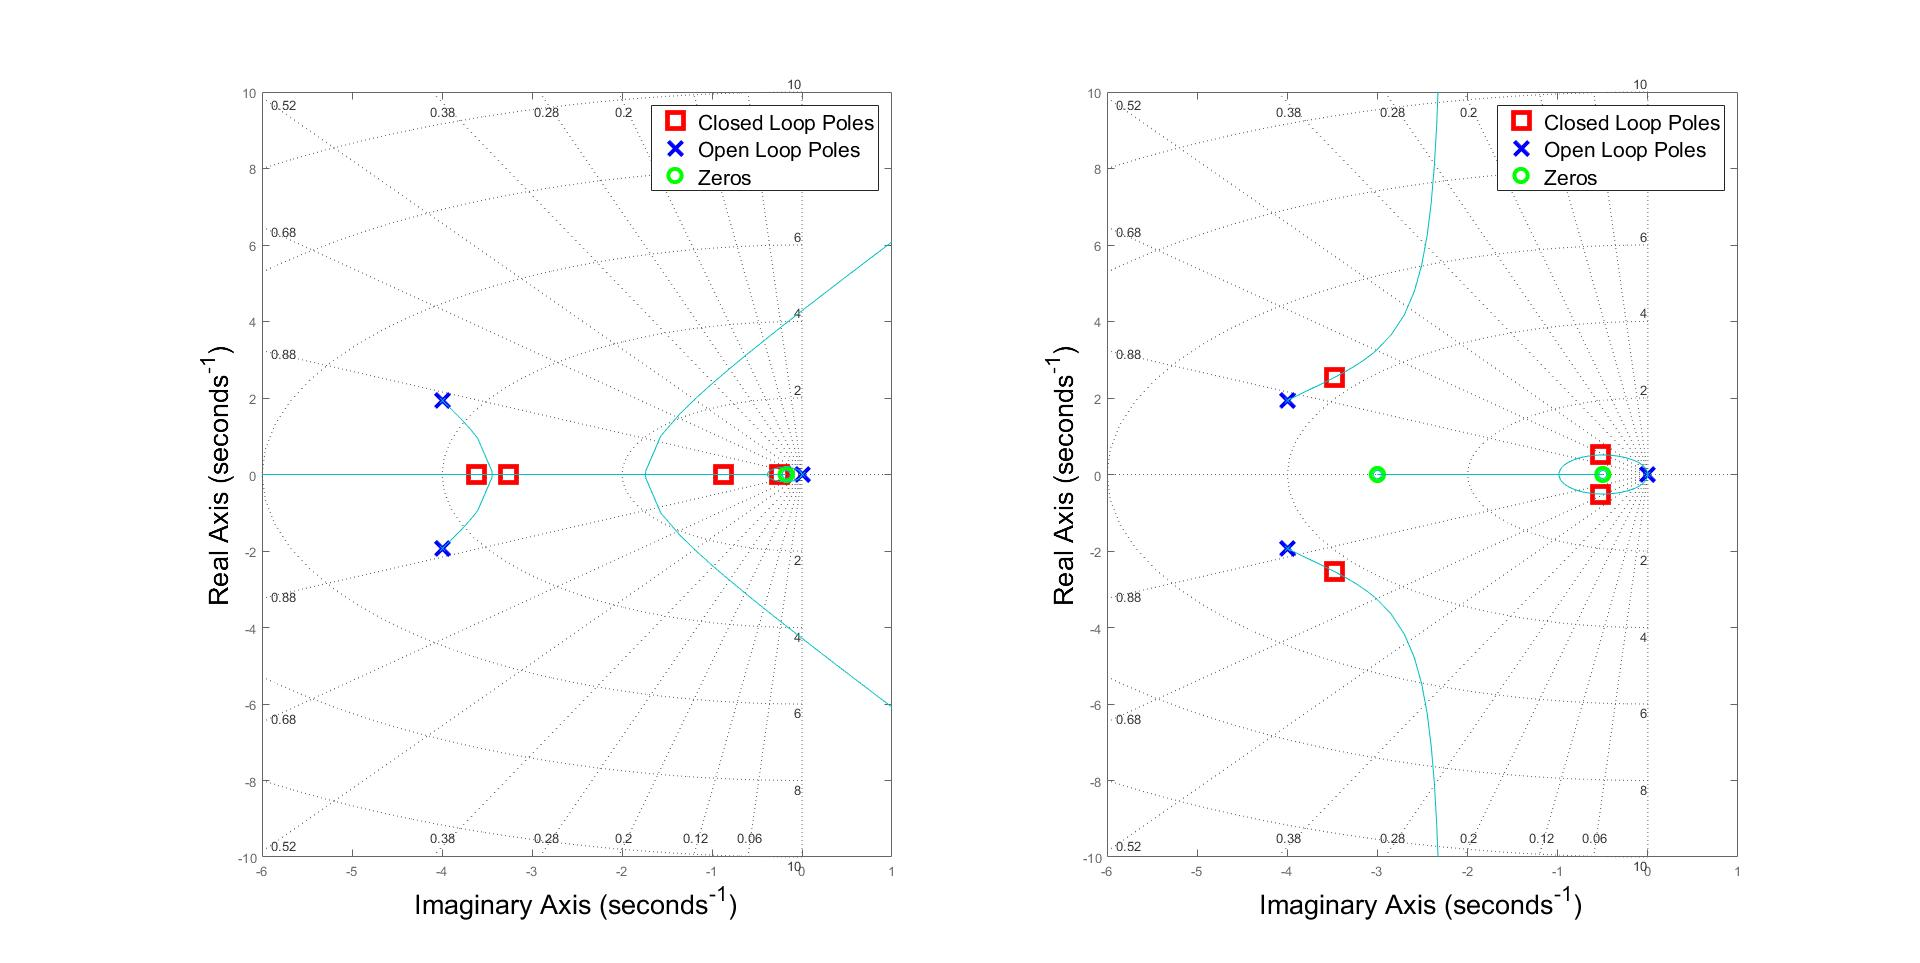
\includegraphics[height = 8cm]{../Design/Matlab/Controllers/yaw_angle_root.jpg}
	\caption{Yaw Angle Controller -  Root Locus (Left:PI, Right:PID)}
	\label{IM_YawAngleControlRoot}
\end{figure}

The frequency response of both systems is evaluated next. Using the open loop bode plots shown in Figure \ref{IM_YawAngleControlBode}, unity feedback is compared with a PI and PID controller. The first zero in both cases is placed close to the origin to limit the effect the new zero has on the system. The PID controller's second zero is placed to increase the phase of the system, allowing for more bandwidth in each leg of the controller. This additional phase allows for larger and more aggressive disturbance rejection, but will result in larger setpoints for the inner yaw rate loop.

The gain of each system has similar bandwidth around the cross over point. The extra zero in the PID controller reduces the gradient of the gain slope off and increases the total phase of the system. The PID controller exhibits the second largest phase margin of $61$\textdegree\ which is found at $1.12$\,rad/s, the fastest of the three crossover frequencies. The PI controller achieves the desired bandwidth and has the slowest crossover frequency of $0.75$\,rad/s, this however relates to a lower phase margin of $59$\textdegree. The final crossover frequency of the yaw rate system was $2.37$\,rad/s, resulting in a ratio with the PID controller of $2.12$ and a ratio of $3.16$ with the PI controller. A larger ratio implies less risk of attenuation for the outer loop.

\begin{figure}[H]
	\centering
	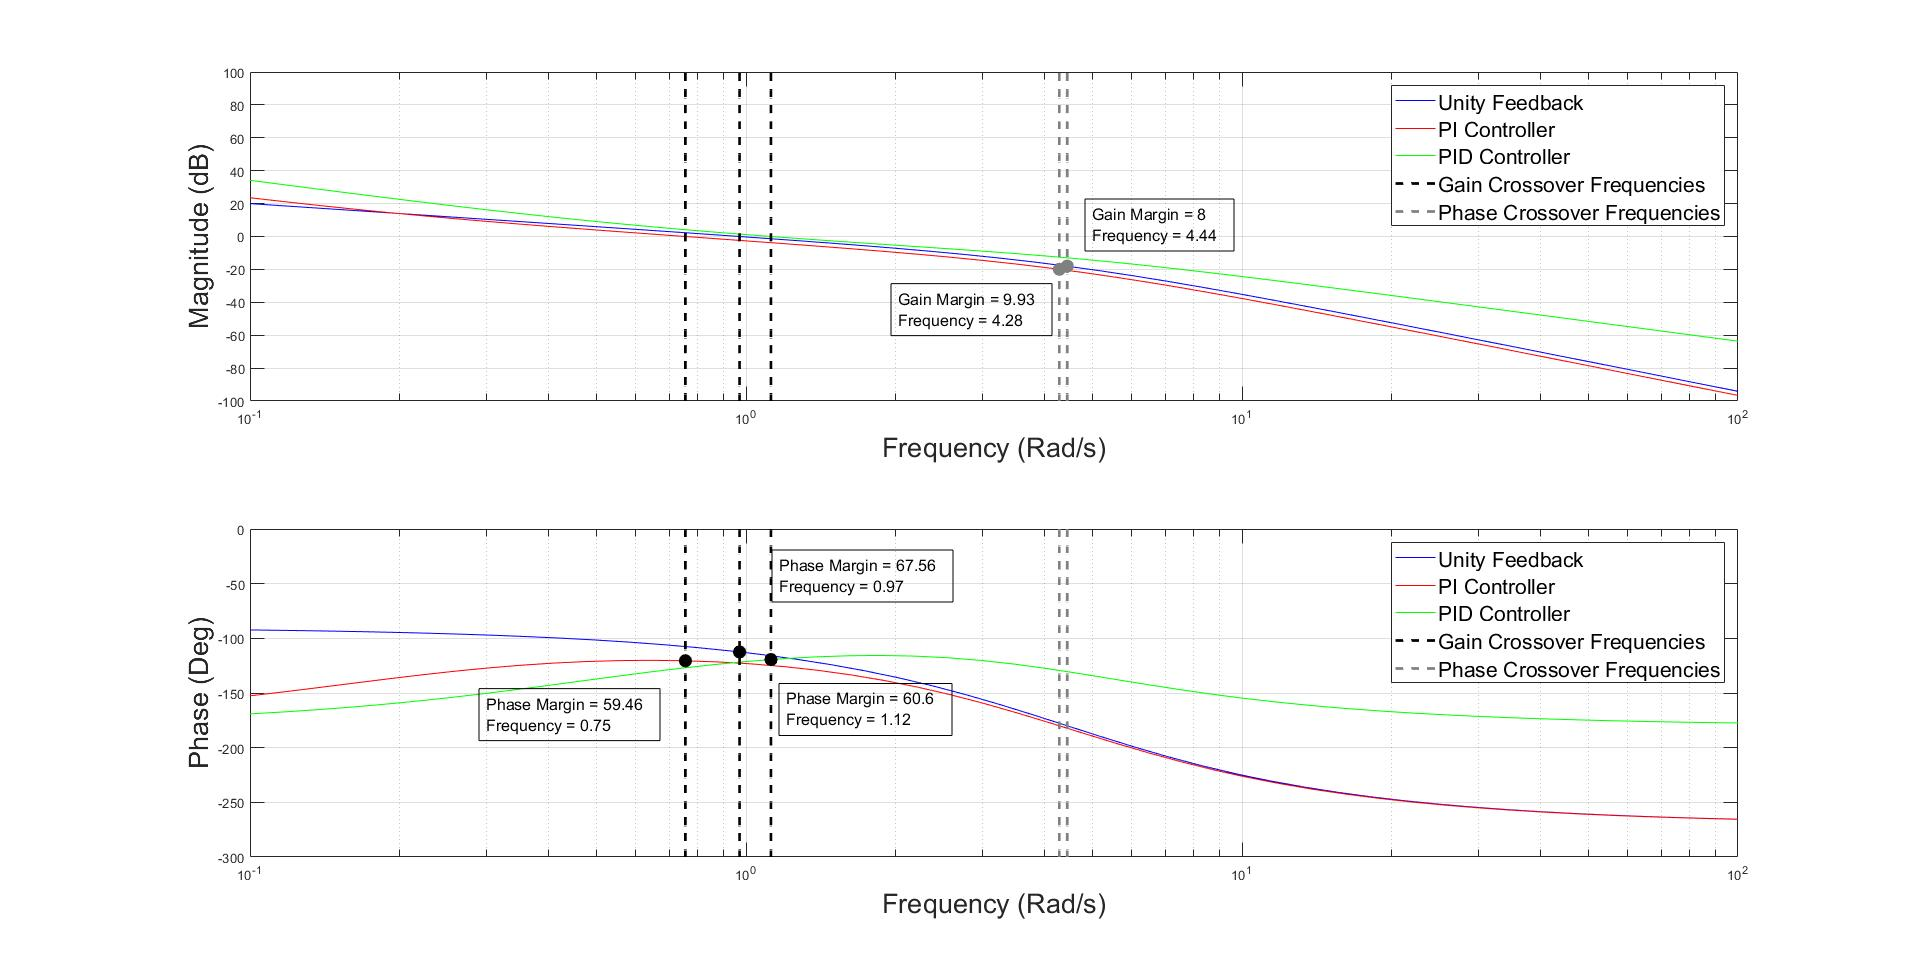
\includegraphics[height = 8cm]{../Design/Matlab/Controllers/yaw_angle_bode.jpg}
	\caption{Yaw Angle Controller -  Bode Plots}
	\label{IM_YawAngleControlBode}
\end{figure}

\subsubsection{Yaw Angle Controller Discussion}	
Each controller was added to the non-linear simulation and evaluated in the time domain including the non linearities previously unconsidered. Figure \ref{IM_YawAngleStep} shows the results of both controllers with and without the limits as well as the additional low pass filter on the differential gain. The PID controller without any limits or low pass filtering had a $5$ \% settling time of $6.37s$, adding in the limits and filter decreases that time to $4.9s$. The PI controller had a settling time of $10.3s$ with no limits which was decreased to $8.8s$ by the addition of the limit on the integrator.

All three systems exhibit some overshoot. The limiters must be carefully chosen to reduce overshoot while also still allowing for substantial disturbance rejection. The linear PI and PID systems produce overshoot of $17$\% and $29$\% respectively. The limits for the integrators on both systems was set to $\pm 0.1$\,rad/s. This limit also becomes the maximum offset this controller can successfully correct for. Both systems had significant overshoot reduction, the PI controller now only had a $12$\% overshoot, with the limited PID system showing only $6$\% overshoot. 

\begin{figure}[H]
	\centering
	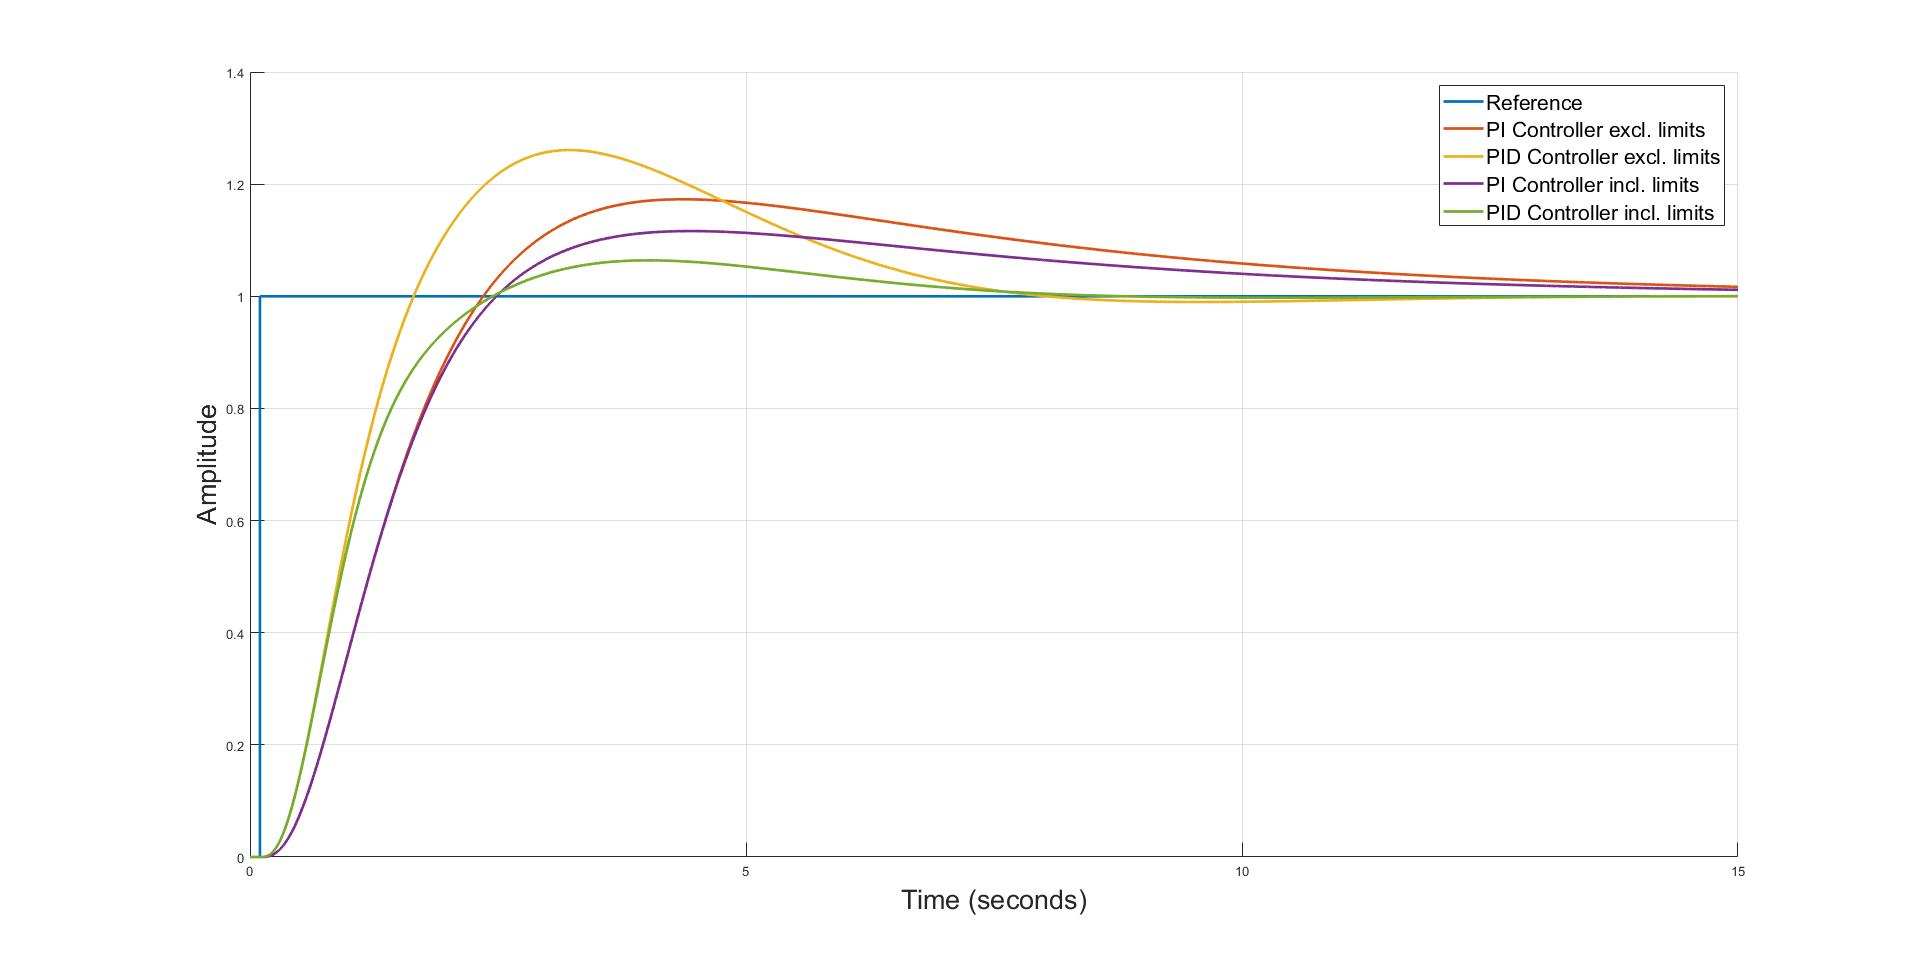
\includegraphics[height = 8cm]{../Design/Matlab/Controllers/yaw_angle_step_both_limits.jpg}
	\caption{Yaw Angle Controller -  Step Responses}
	\label{IM_YawAngleStep}
\end{figure}

As mentioned the limits introduce the maximum disturbance rejection capability of each system. Figure \ref{IM_YawAngleStepBoth} shows how each limited system handles a measurement offset of $0.1$\,rad/s in the yaw rate loop.

\begin{figure}[H]
	\centering
	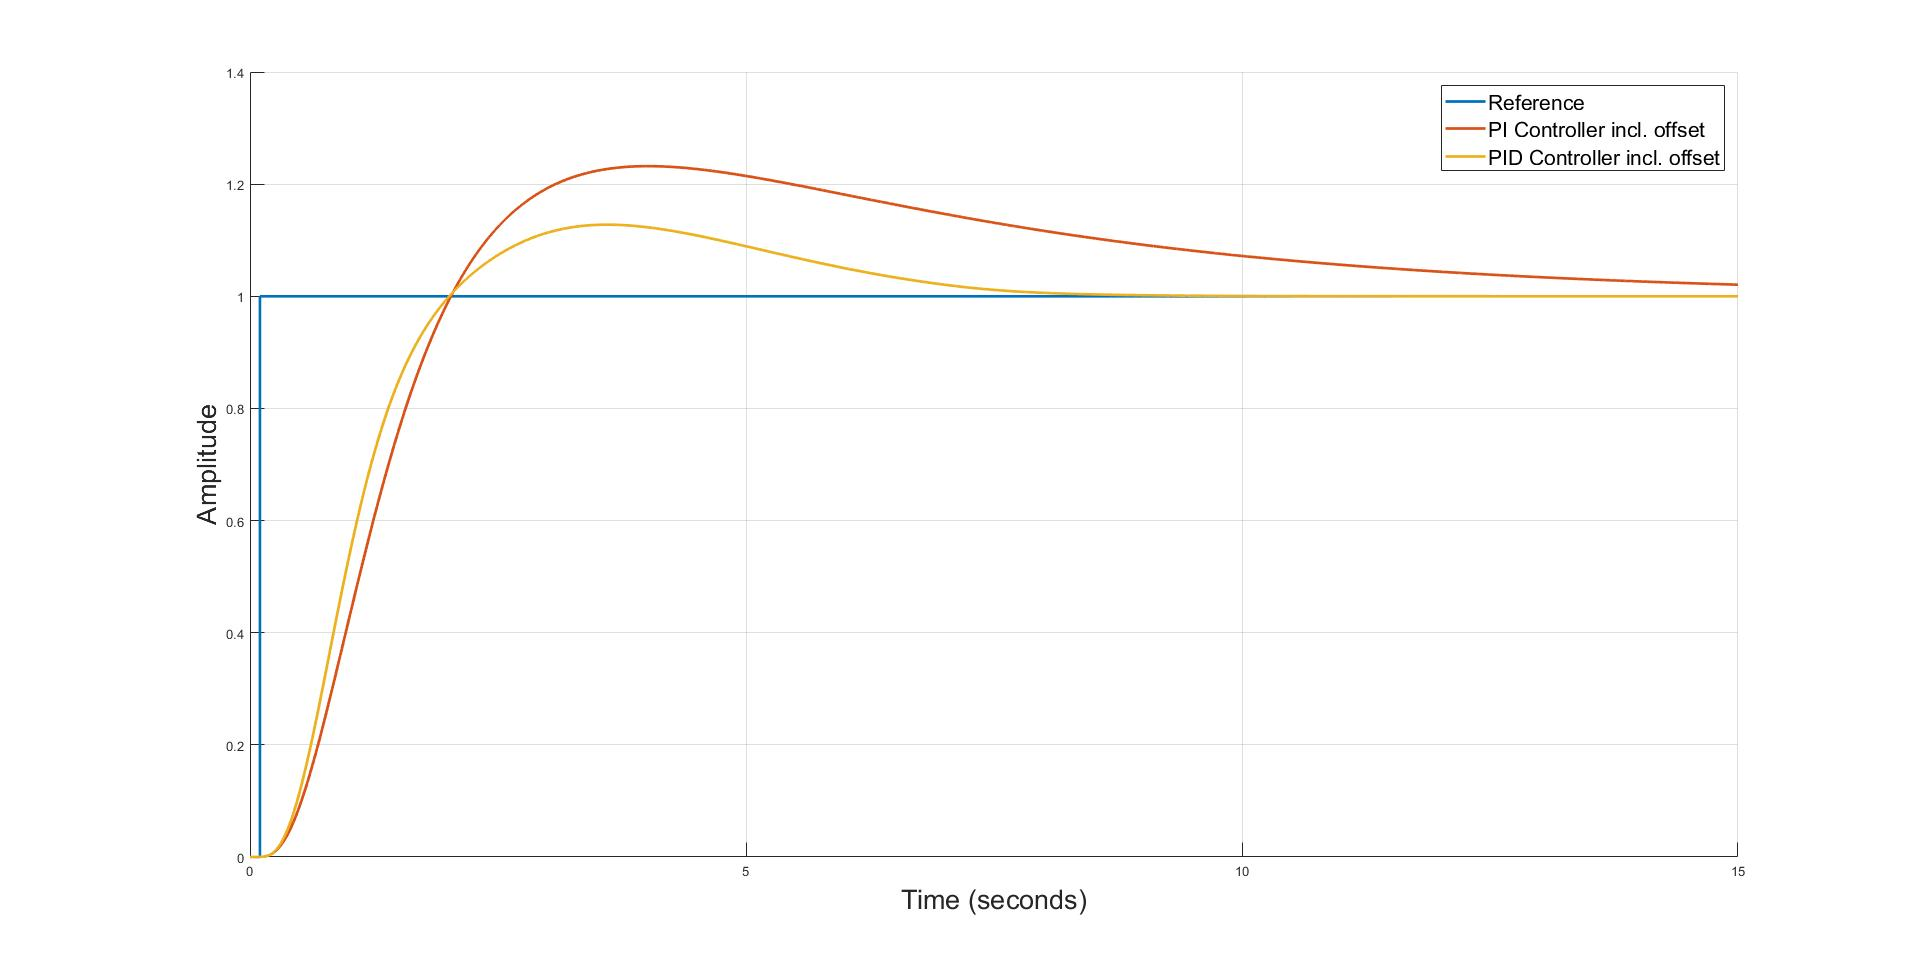
\includegraphics[height = 8cm]{../Design/Matlab/Controllers/yaw_angle_step_both_dist.jpg}
	\caption{Yaw Angle Controller -  Step Responses Including Inner Loop Measurement Offset}
	\label{IM_YawAngleStepBoth}
\end{figure}

The final consideration is the impulse each system creates for the yaw rate controller, Figure \ref{IM_YawAngleImpulse} demonstrates both limited systems impulse responses. As seen the PID controller commands a larger initial setpoint, more than double that of the PI controller.    

\begin{figure}[H]
	\centering
	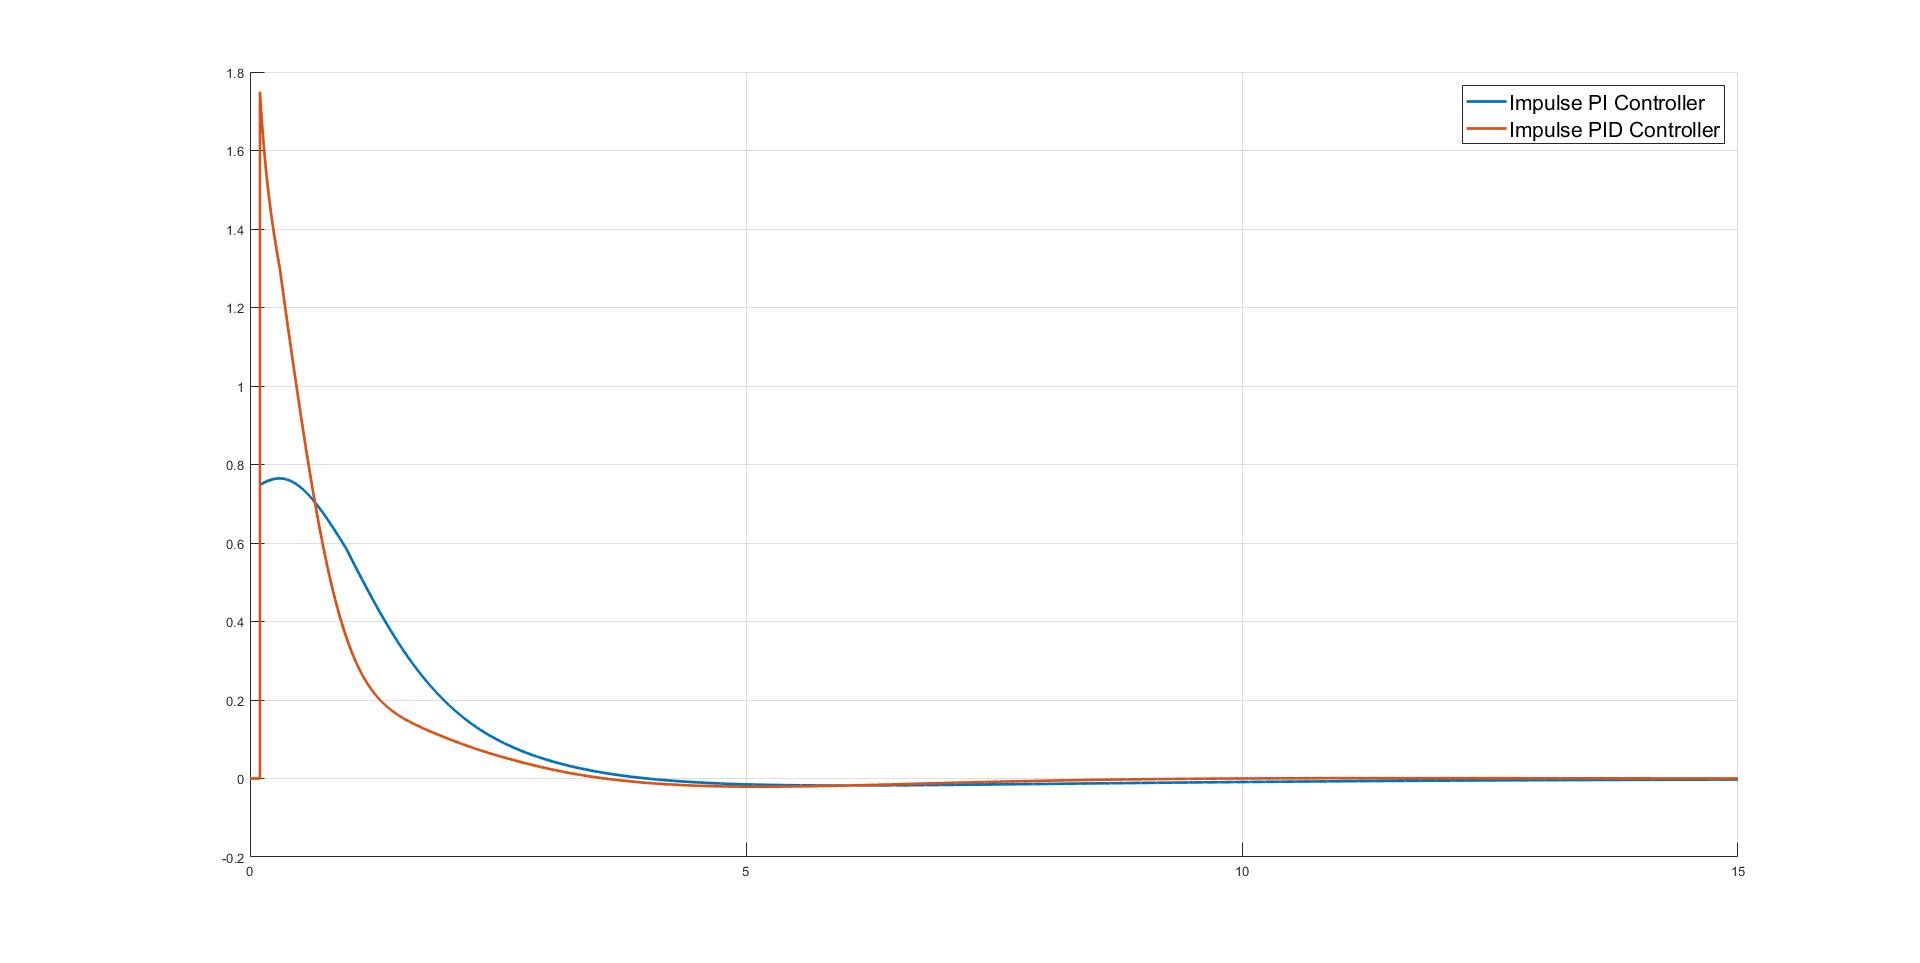
\includegraphics[height = 8cm]{../Design/Matlab/Controllers/yaw_angle_impulse.jpg}
	\caption{Yaw Angle Controller -  Impulses}
	\label{IM_YawAngleImpulse}
\end{figure}

The PI controller is chosen as the final controller implementation for the yaw angle loop. 


\end{document}   